
På baggrund af simuleringer med Inundation Modellen og analysering af resultaterne præsenteres resultaterne af 2023-stormflods simuleringen, påvirkede arealanvendelser og simuleringerne af fremtidige klimascenarier på baggrund af en statistisk 100-års hændelse og en fremskrevet stormflod ved et SSP4,5 og 8,5 udledningsscenarie. 

\subsection{Simuleringen af oktober 2023 stormfloden}
Figur \ref{Subfig: Målt Aabenraa} viser det oversvømmelseskort Aabenraa kommune har udarbejdet, der viser den observerede hændelse fra stormfloden og figur \ref{Subfig: Model Aabenraa} viser resultatet af simuleringen af stormfloden fra Inundation Modellen for Aabenraa. \\
Der er forskel mellem de to resultater. Modellens resultat er større især vest for lystbådhavnen ved et større rekreativt område og et bebygget område. Modellen resulterede i et areal på 129,8 ha, mens det observeret areal var på 70,1 ha. Dette medfører i at modellens resultat er 83,5\% større end den observeret hændelse, svarende til ca. 59 ha.
\begin{figure}[H]
    \begin{subfigure}[t]{0.5\textwidth}
        \centering
        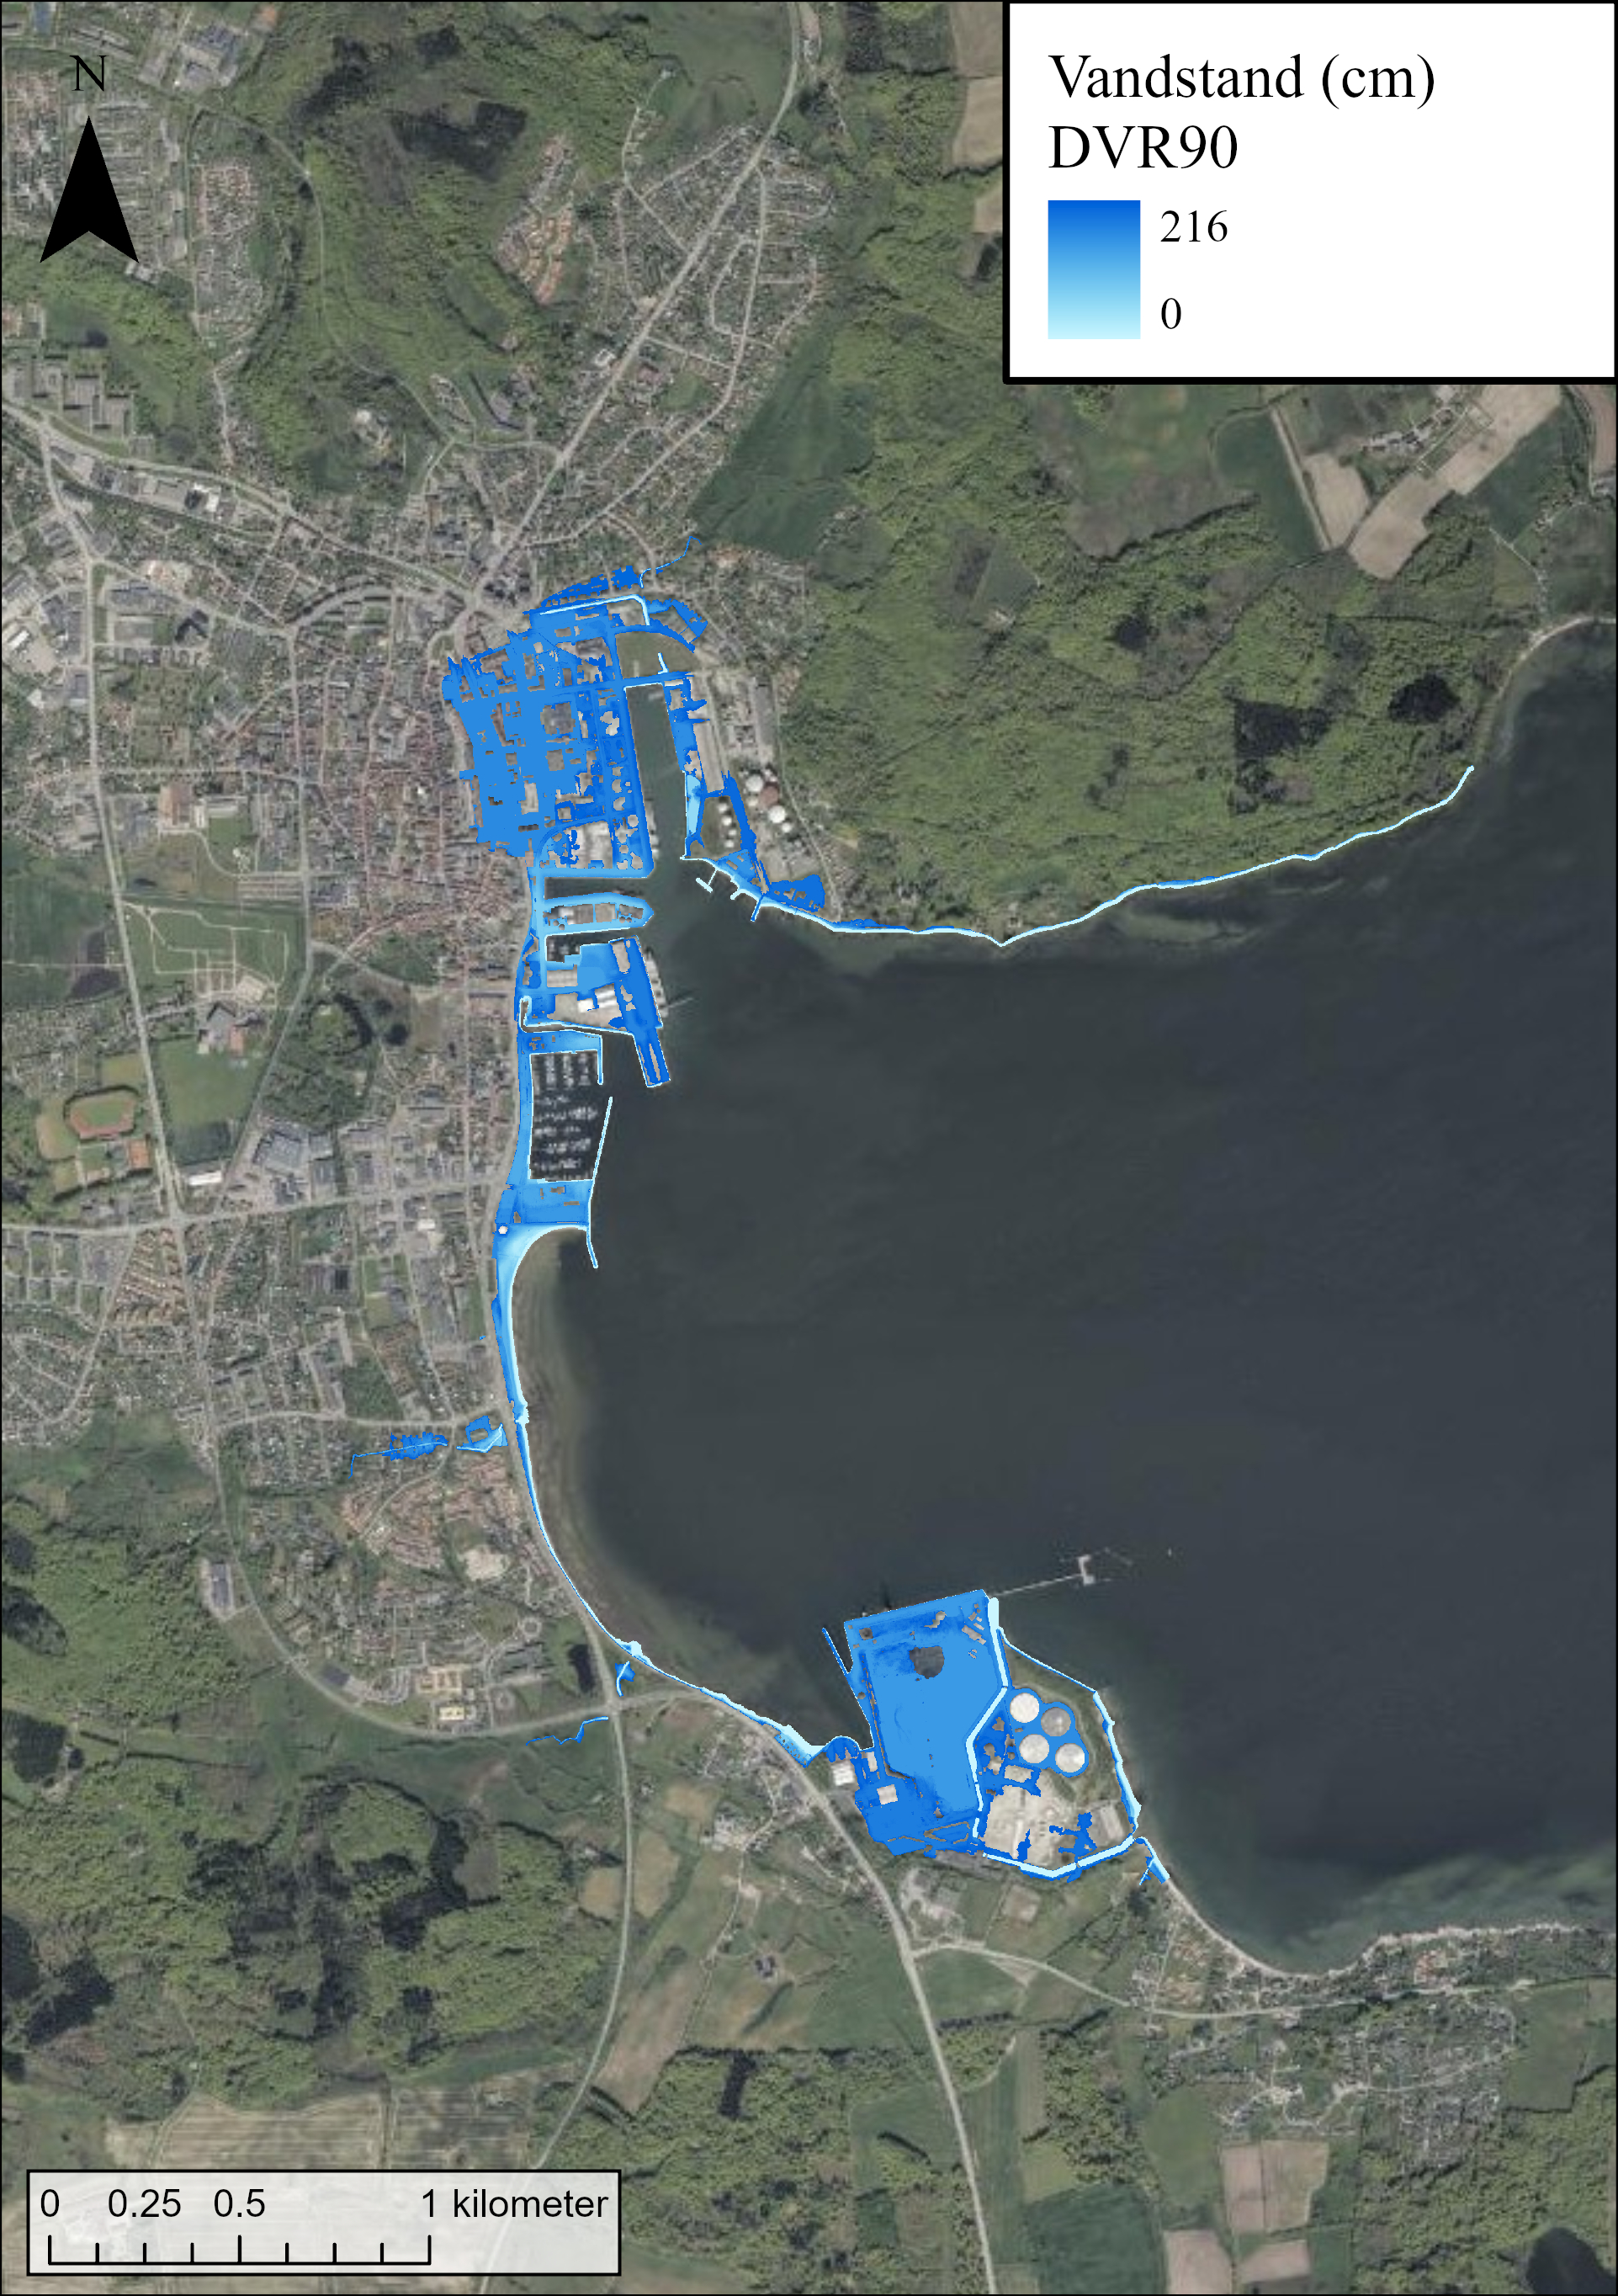
\includegraphics[width=0.95\linewidth]{images/Resultater/2023Malt/2023 resultat_aabenraa.jpg}
        \caption{}
        \label{Subfig: Målt Aabenraa}
    \end{subfigure}
    \begin{subfigure}[t]{0.5\textwidth}
        \centering
        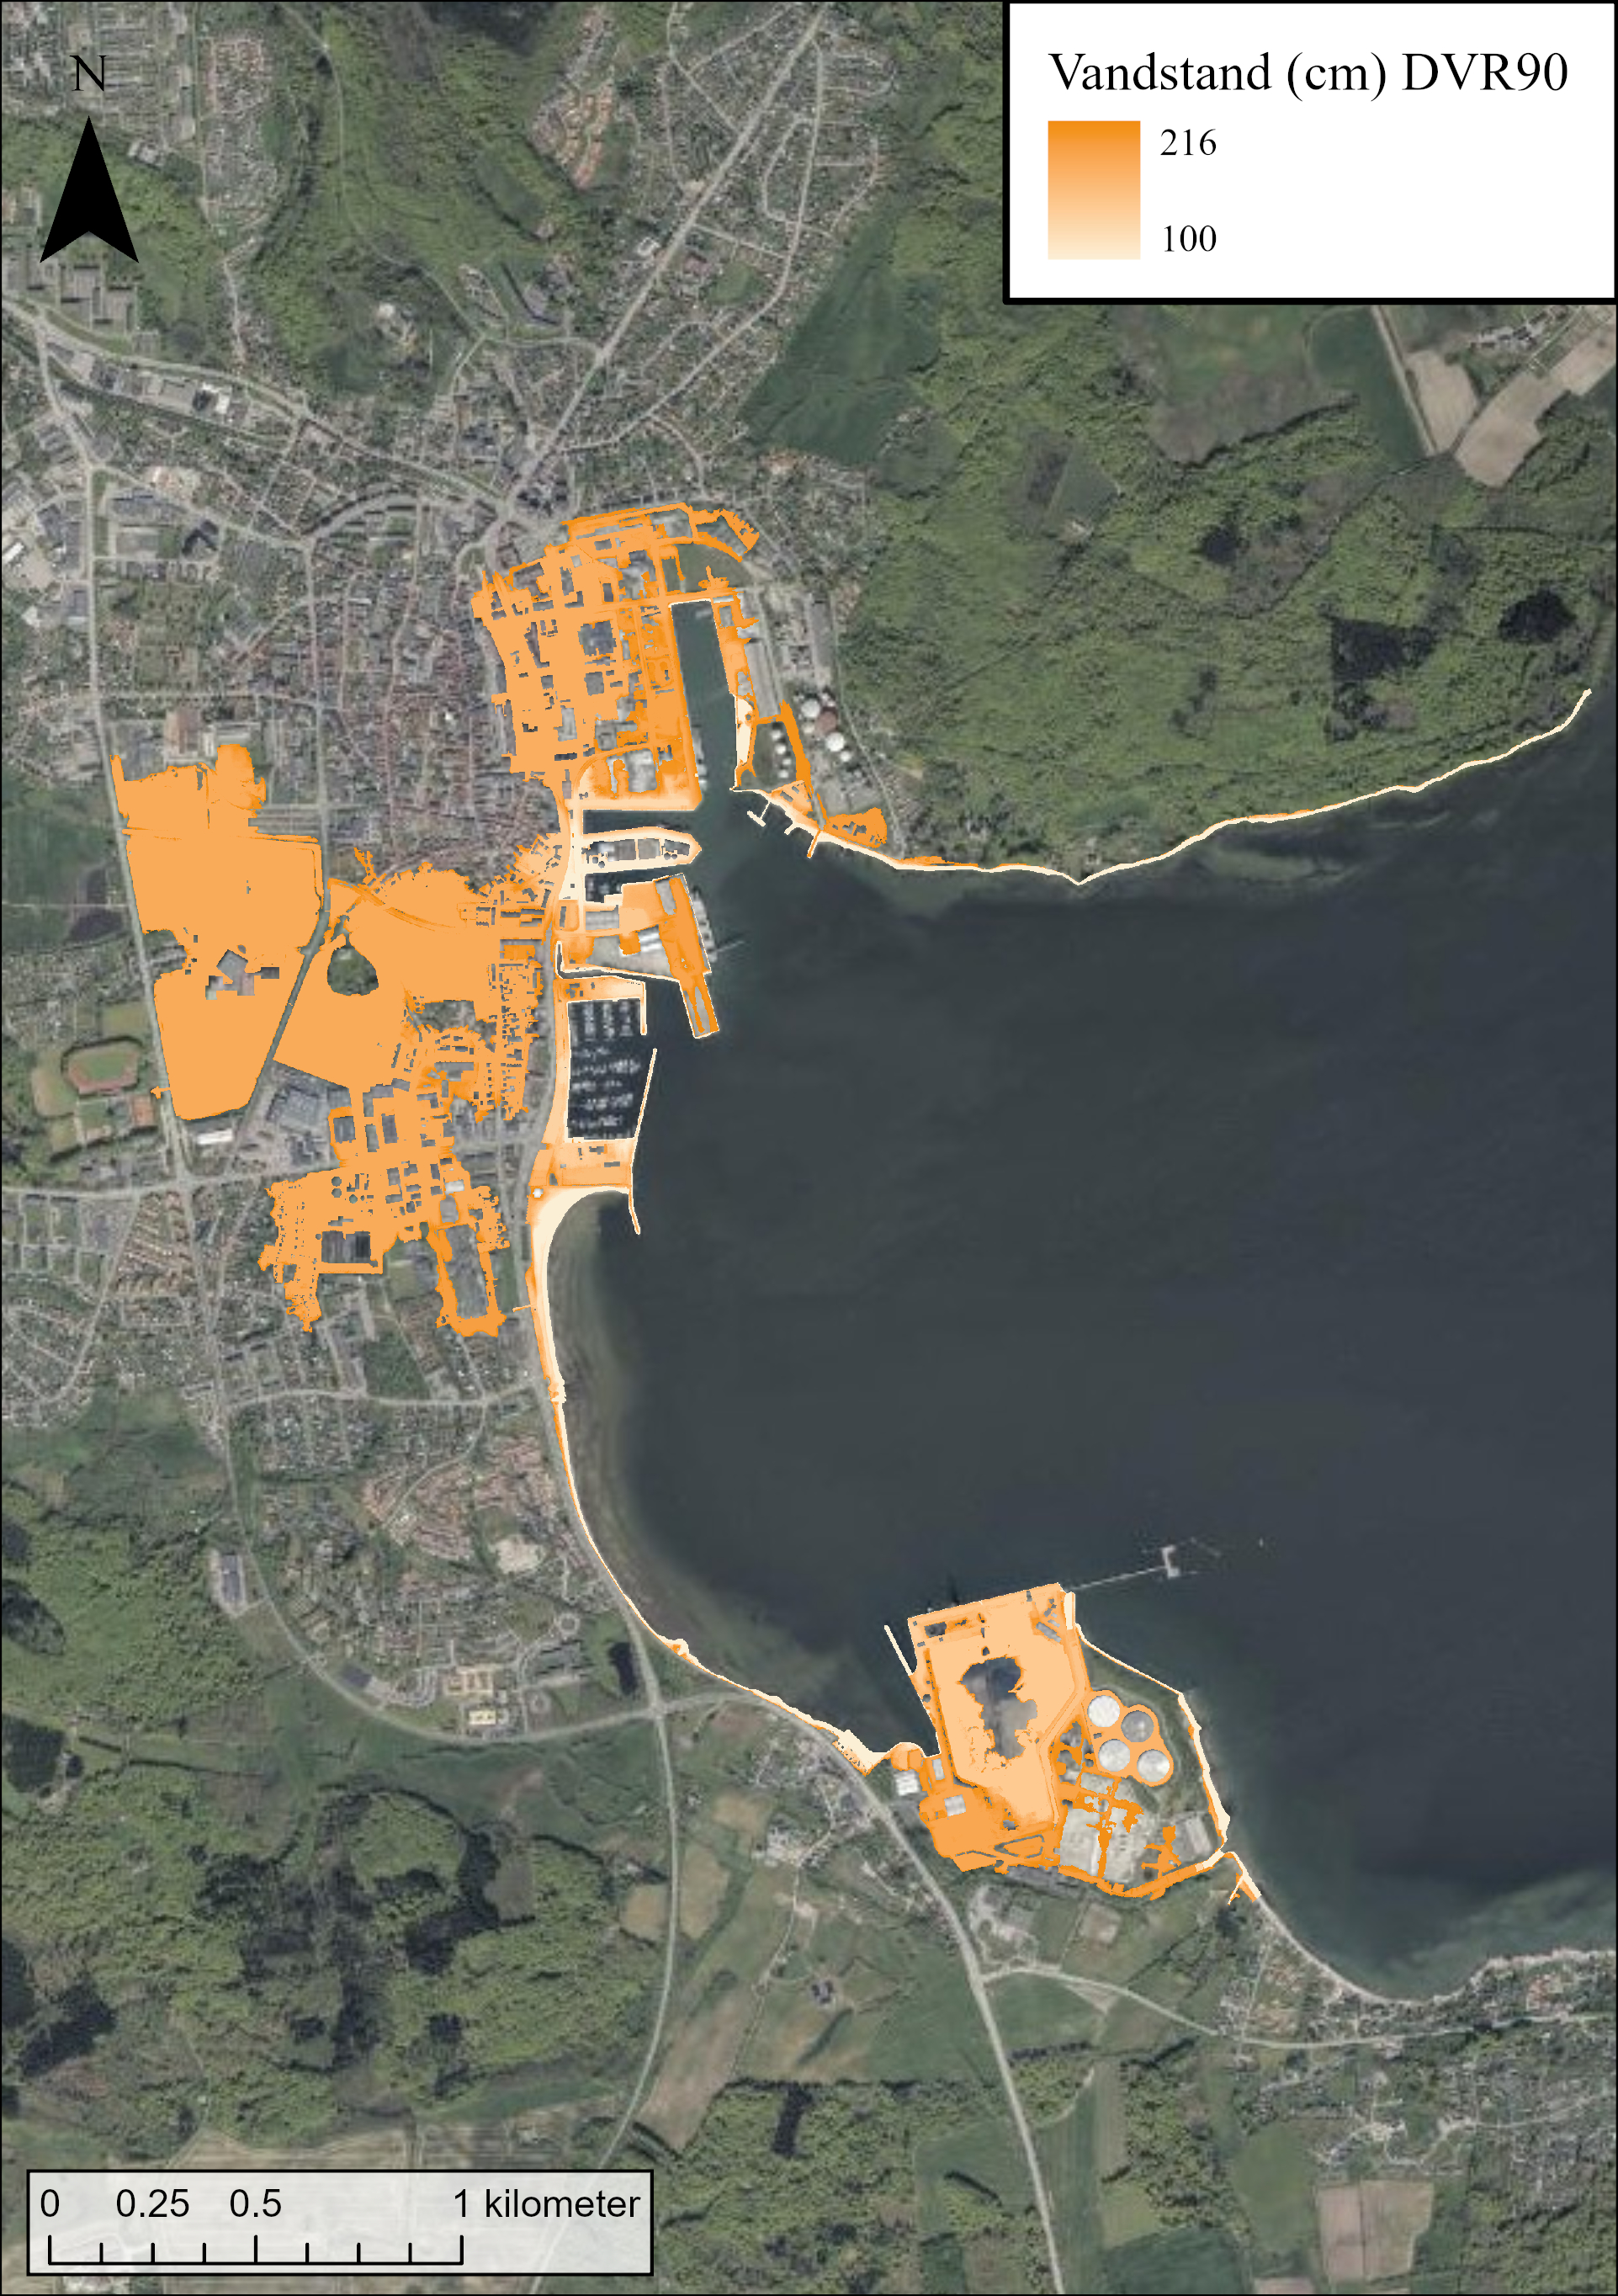
\includegraphics[width=0.95\linewidth]{images/Resultater/2023Model/2023 model_aabenraa.jpg}
        \caption{}
        \label{Subfig: Model Aabenraa}
    \end{subfigure}
    \caption{Oversvømmelseskort over oktober 2023-stormfloden for Aabenraa. \textbf{(a)} Observeret data og \textbf{(b)} Simuleret data}
    \label{Figur: Målt & simuleret Aabenraa}
\end{figure}
Stormfloden i Aabenraa påvirkede syv forskellige arealanvendelser. I figur \ref{Subfig: Arealklasser i procent Aabenraa} er der vist hvilke arealer der blev påvirket under den observeret og simuleret stormflod, som procent af det totale oversvømmet areal. Under den observeret stormflod blev 42\% af bebyggede områder oversvømmet, svarende til 30 ha (figur \ref{Subfig: Hektar arealklasser Aabenraa}). Hvorimod ved den simuleret stormflod blev 29\% af det bebyggede areal oversvømmet, svarende til ca. 37 ha (figur \ref{Subfig: Hektar arealklasser Aabenraa}). En anden klasse hvor der er forskel mellem resultaterne er rekreativt areal, hvor 25 ha oversvømmes i den simuleret stormflod, svarende til ca. 20\% af det totale areal. I modsætning til den observeret stormflod hvor 0,41 ha (0,6\%) af rekreativ areal blev oversvømmet.
\begin{figure}[H]
    \begin{subfigure}[t]{0.5\textwidth}
        \centering
        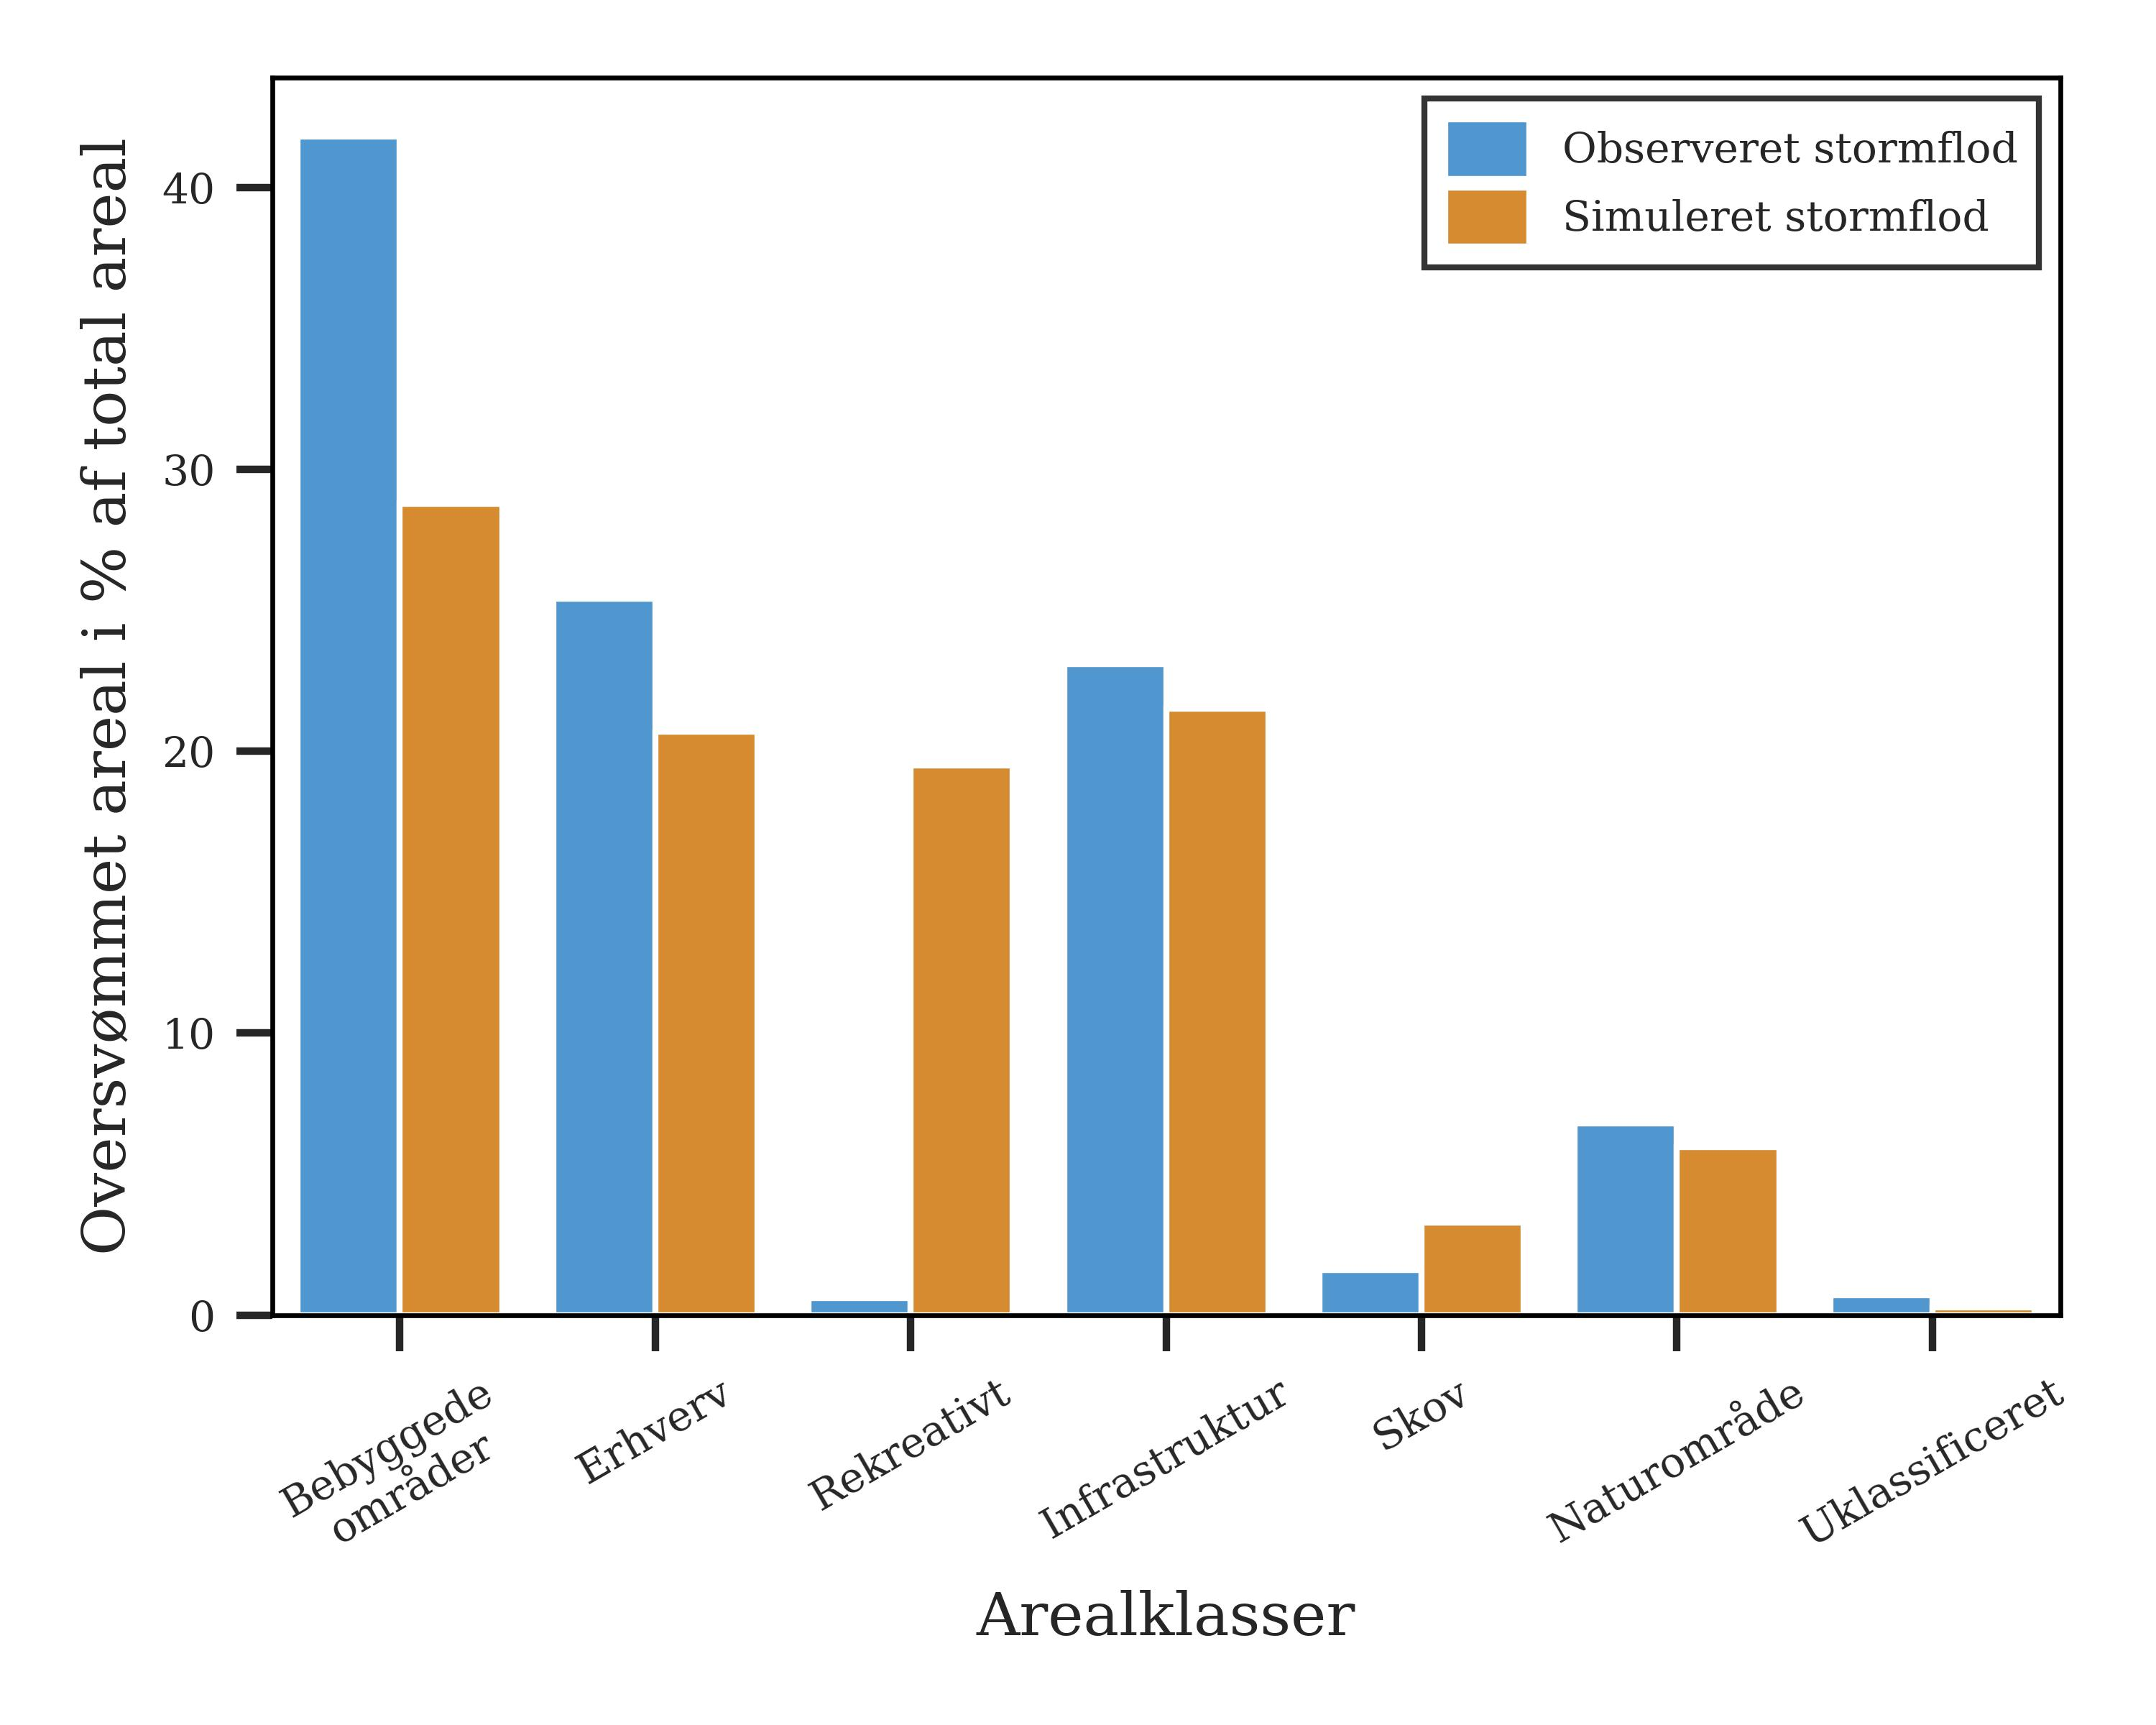
\includegraphics[width=1\linewidth]{images/Resultater/areal_anvendelses_grafer/aabenraa_arealanvendelse.jpg}
        \caption{}
        \label{Subfig: Arealklasser i procent Aabenraa}
    \end{subfigure}
    \begin{subfigure}[t]{0.5\textwidth}
        \centering
        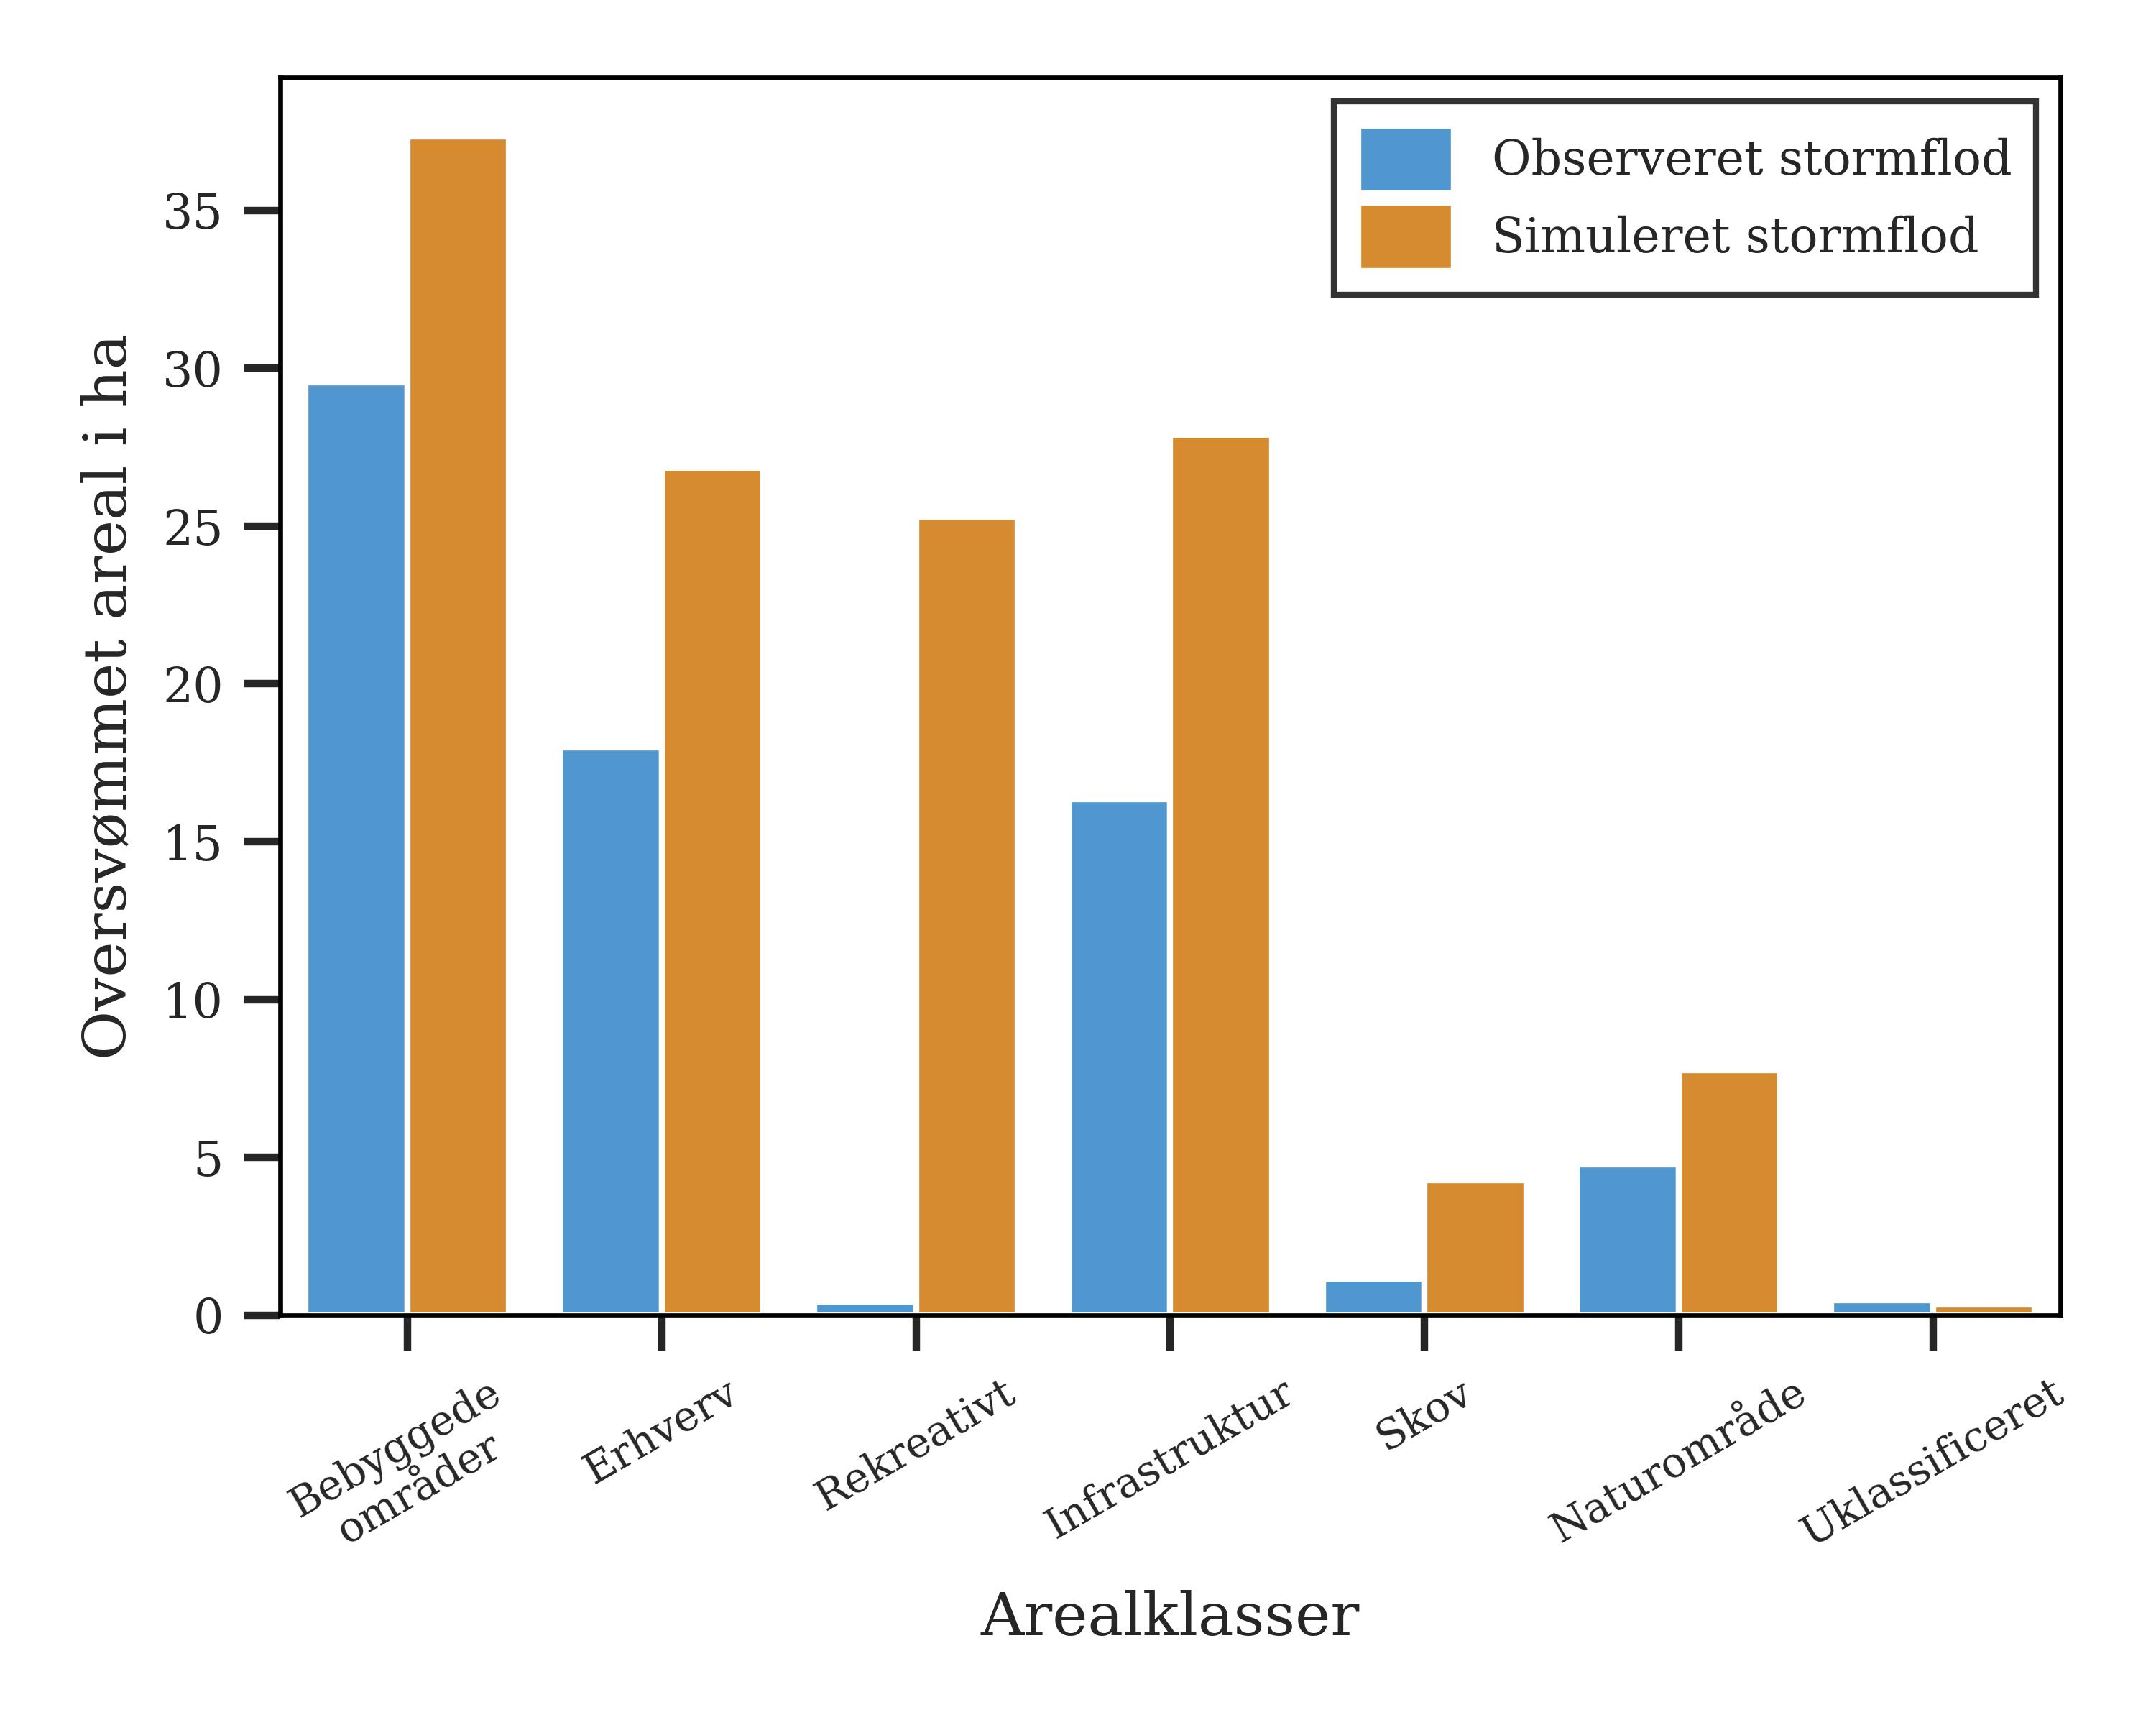
\includegraphics[width=1\linewidth]{images/Resultater/areal_anvendelses_grafer/aabenraa_oversvommet_Hektar.jpg}
        \caption{}
        \label{Subfig: Hektar arealklasser Aabenraa}
    \end{subfigure}
    \caption{Påvirkede arealanvendelsesklasser i Aabenraa for den observeret og simuleret stormflod. \textbf{(a)} Oversømmet areal som procent af det totale areal. \textbf{(b)} Oversvømmet areal i hektar.}
    \label{Figur: Påvirket arealanvendelse Aabenraa}
\end{figure}

På figur \ref{Subfig: Målt Gedser} ses arealet af den observeret oversvømmelse af Gedser Havn af stormfloden. På figur \ref{Subfig: Model Gedser} er det simulerede resultat. Resultatet fra Inundation Modellen er ens med den observeret hændelse. Den observeret hændelse havde et oversvømmet areal på 34,5 ha kontra 33,2 ha fra Inundation Modellen. Modellens resultat er dermed ca. 4\% mindre, svarende til ca. 1,3 ha.  

\begin{figure}[H]
    \begin{subfigure}[t]{0.5\textwidth}
        \centering
        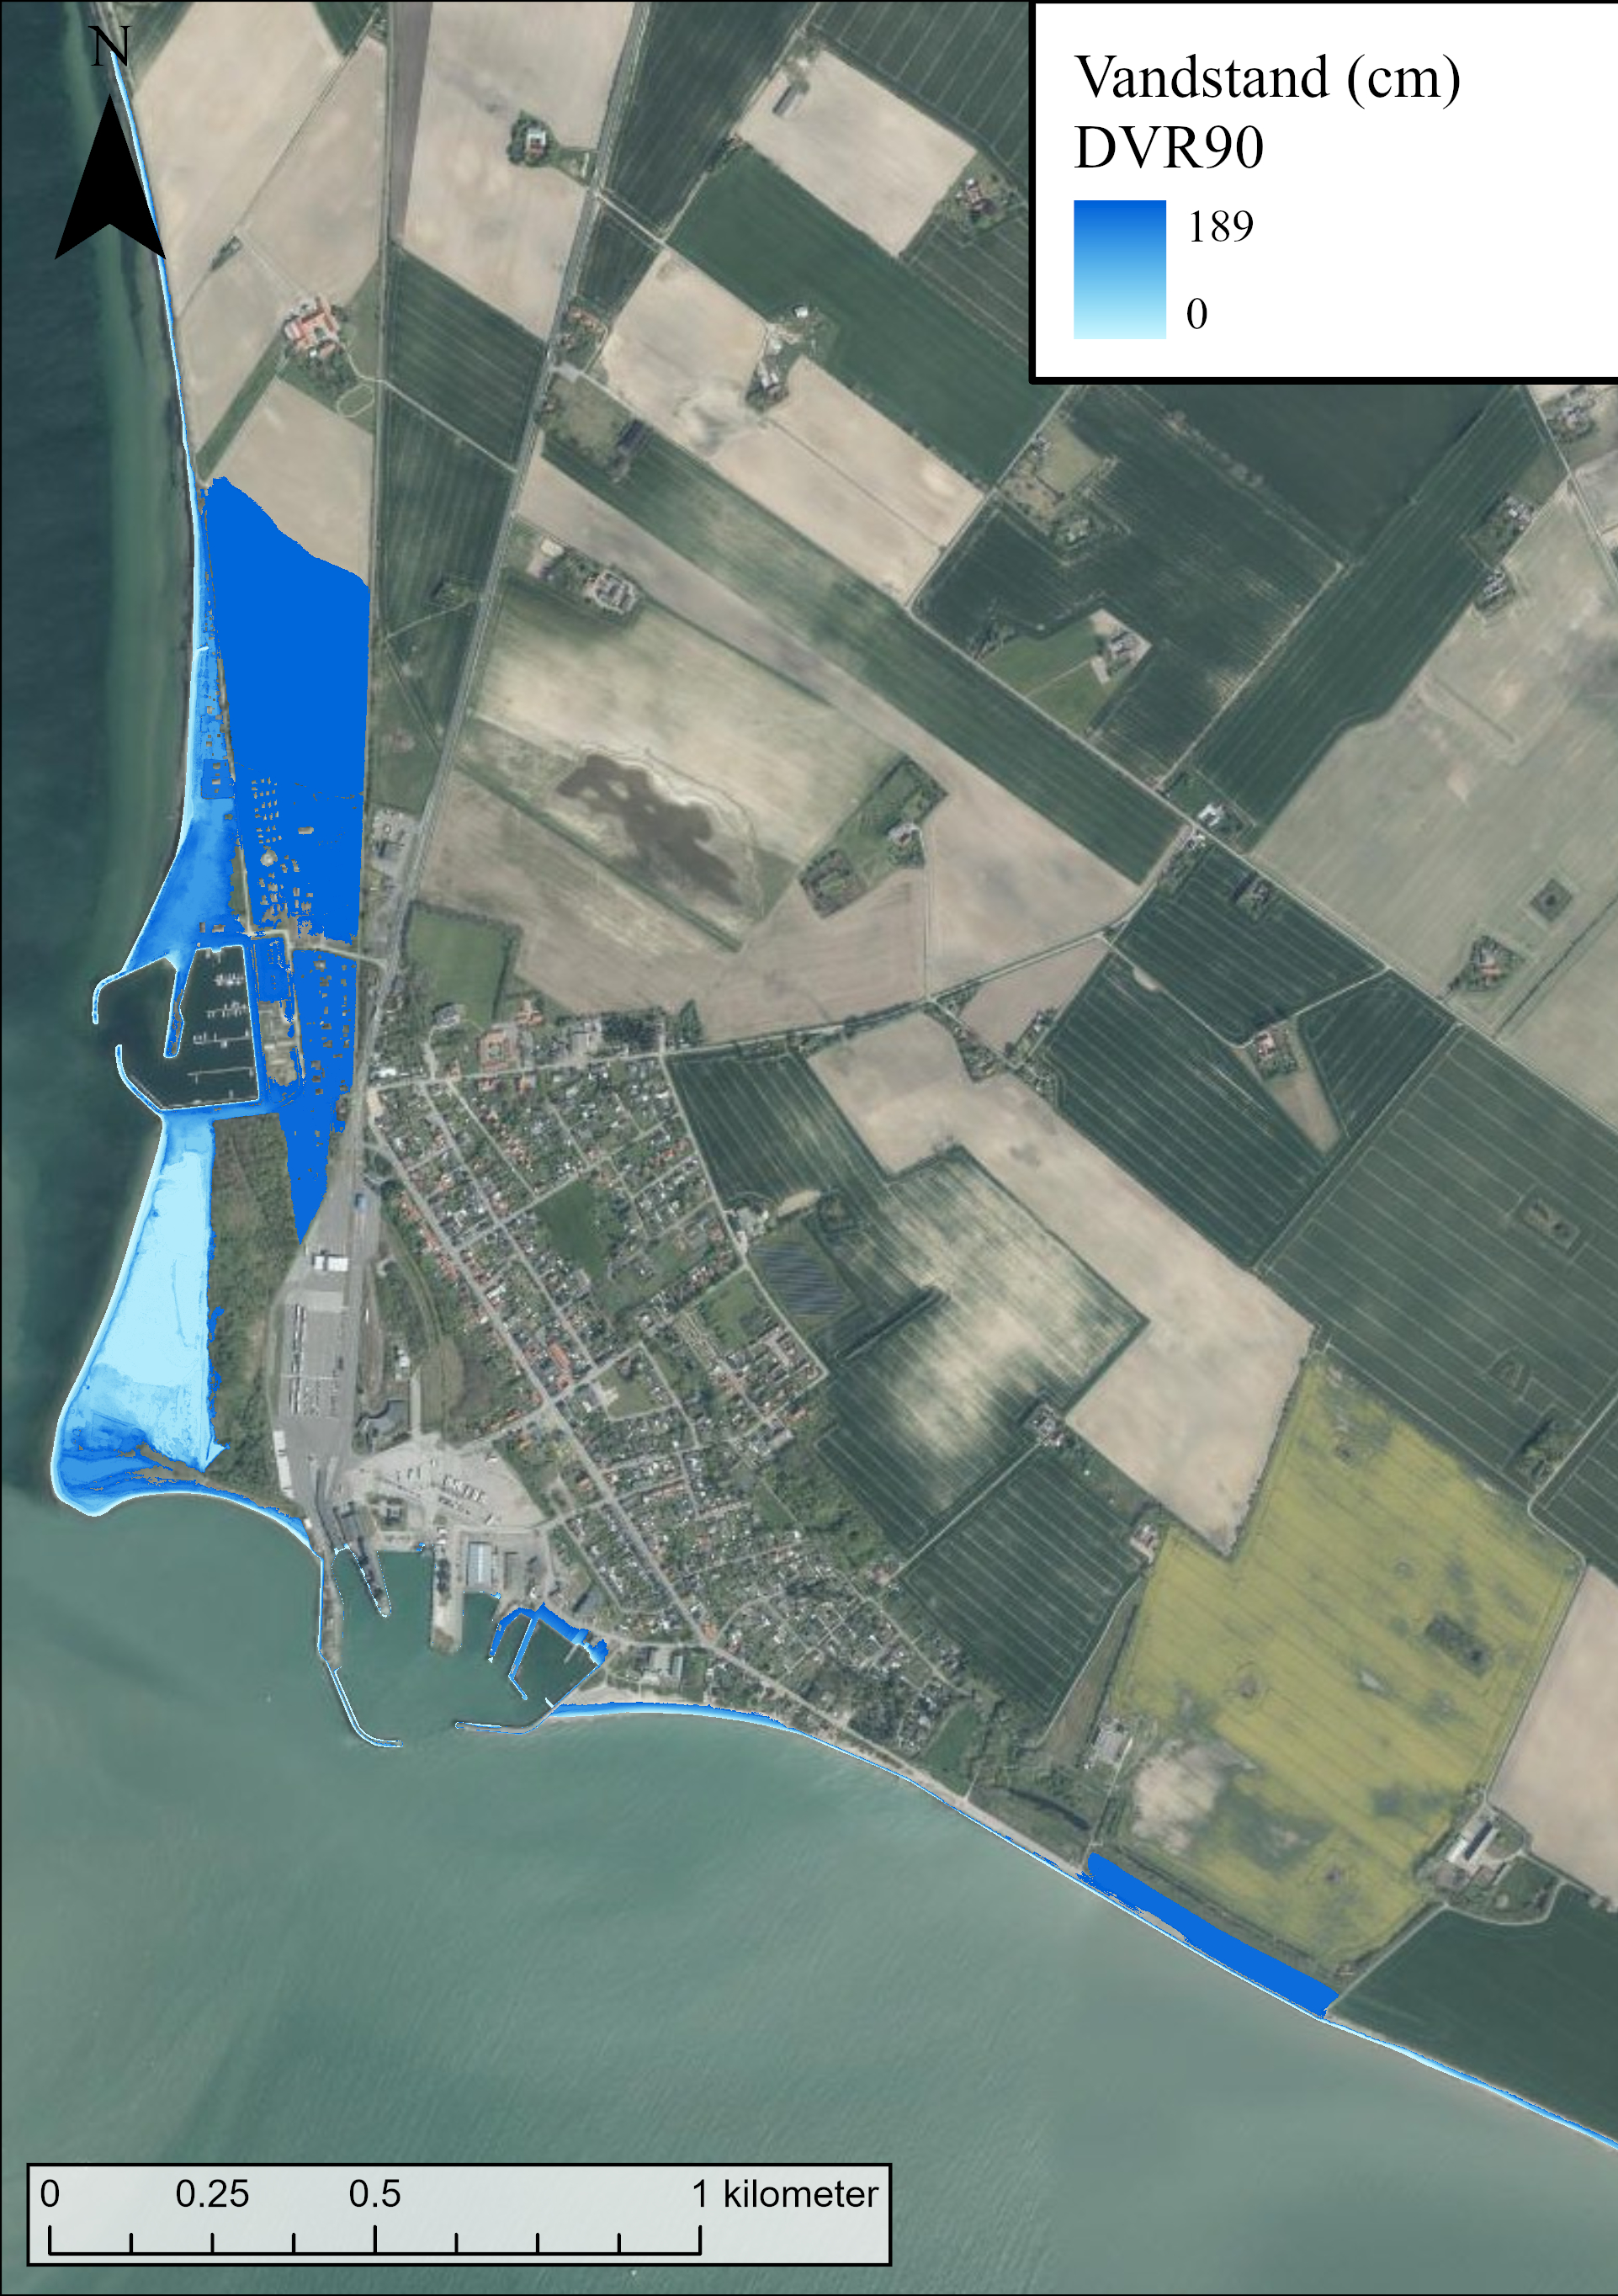
\includegraphics[width=0.95\linewidth]{images/Resultater/2023Malt/2023 resultat_gedser.jpg}
        \caption{}
        \label{Subfig: Målt Gedser}
    \end{subfigure}
    \begin{subfigure}[t]{0.5\textwidth}
        \centering
        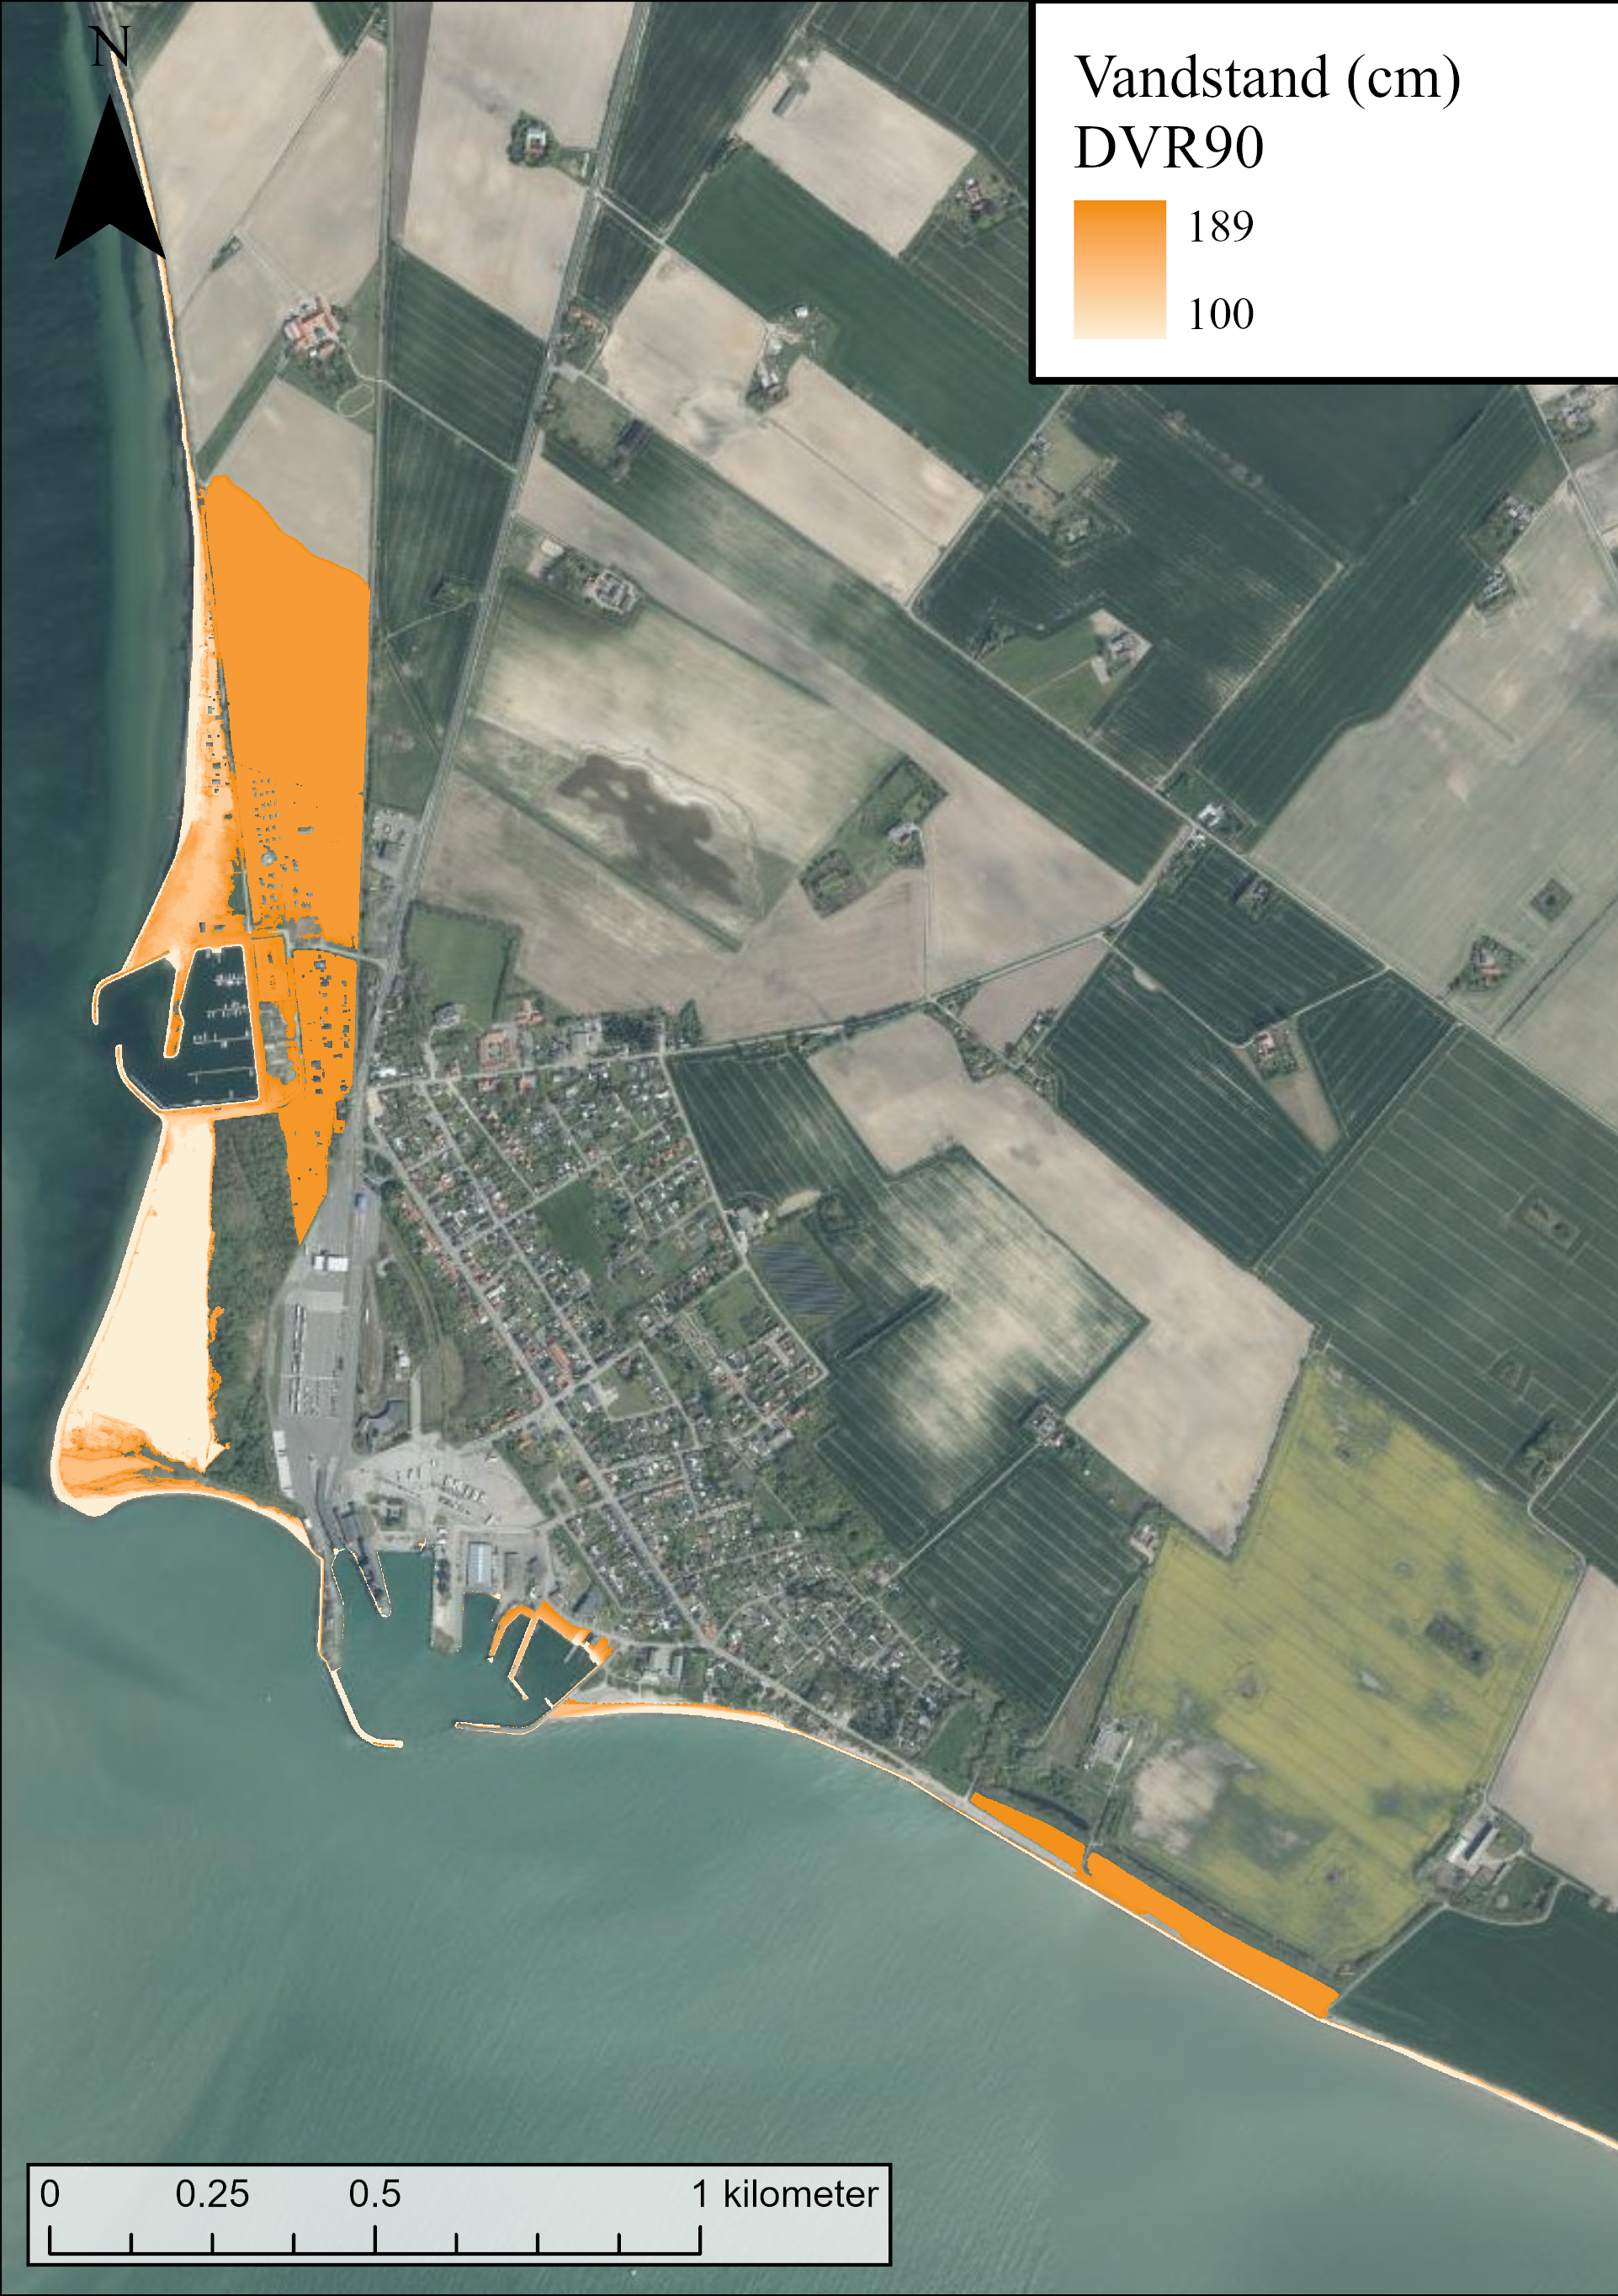
\includegraphics[width=0.95\linewidth]{images/Resultater/2023Model/2023 model_gedser.jpg}
        \caption{}
        \label{Subfig: Model Gedser}
    \end{subfigure}
    \caption{Oversvømmelseskort over oktober 2023 stormfloden for Gedser Havn. \textbf{(a)} Observeret data. \textbf{(b)} Simuleret data}
    \label{Figur: Målt & simuleret Gedser}
\end{figure}

I Gedser Havn blev otte arealklasser påvirket af oversvømmelserne under stormfloden. Ved både den observeret og simuleret stormflod er det naturområder der blev mest påvirket med 17,7 og 17,2 ha, svarende til henholdsvis 51,5 og 51,7\% af det samlet areal (figur \ref{Subfig: Procent areal Gedser} og \ref{Subfig: Hektar areal Gedser}).
Andelen og arealet af de andre oversvømmet arealer er ens for begge resultater (figur \ref{Figur: Påvirket arealanvendelse Gedser}).
\begin{figure}[H]
    \begin{subfigure}[b]{0.5\textwidth}
        \centering
        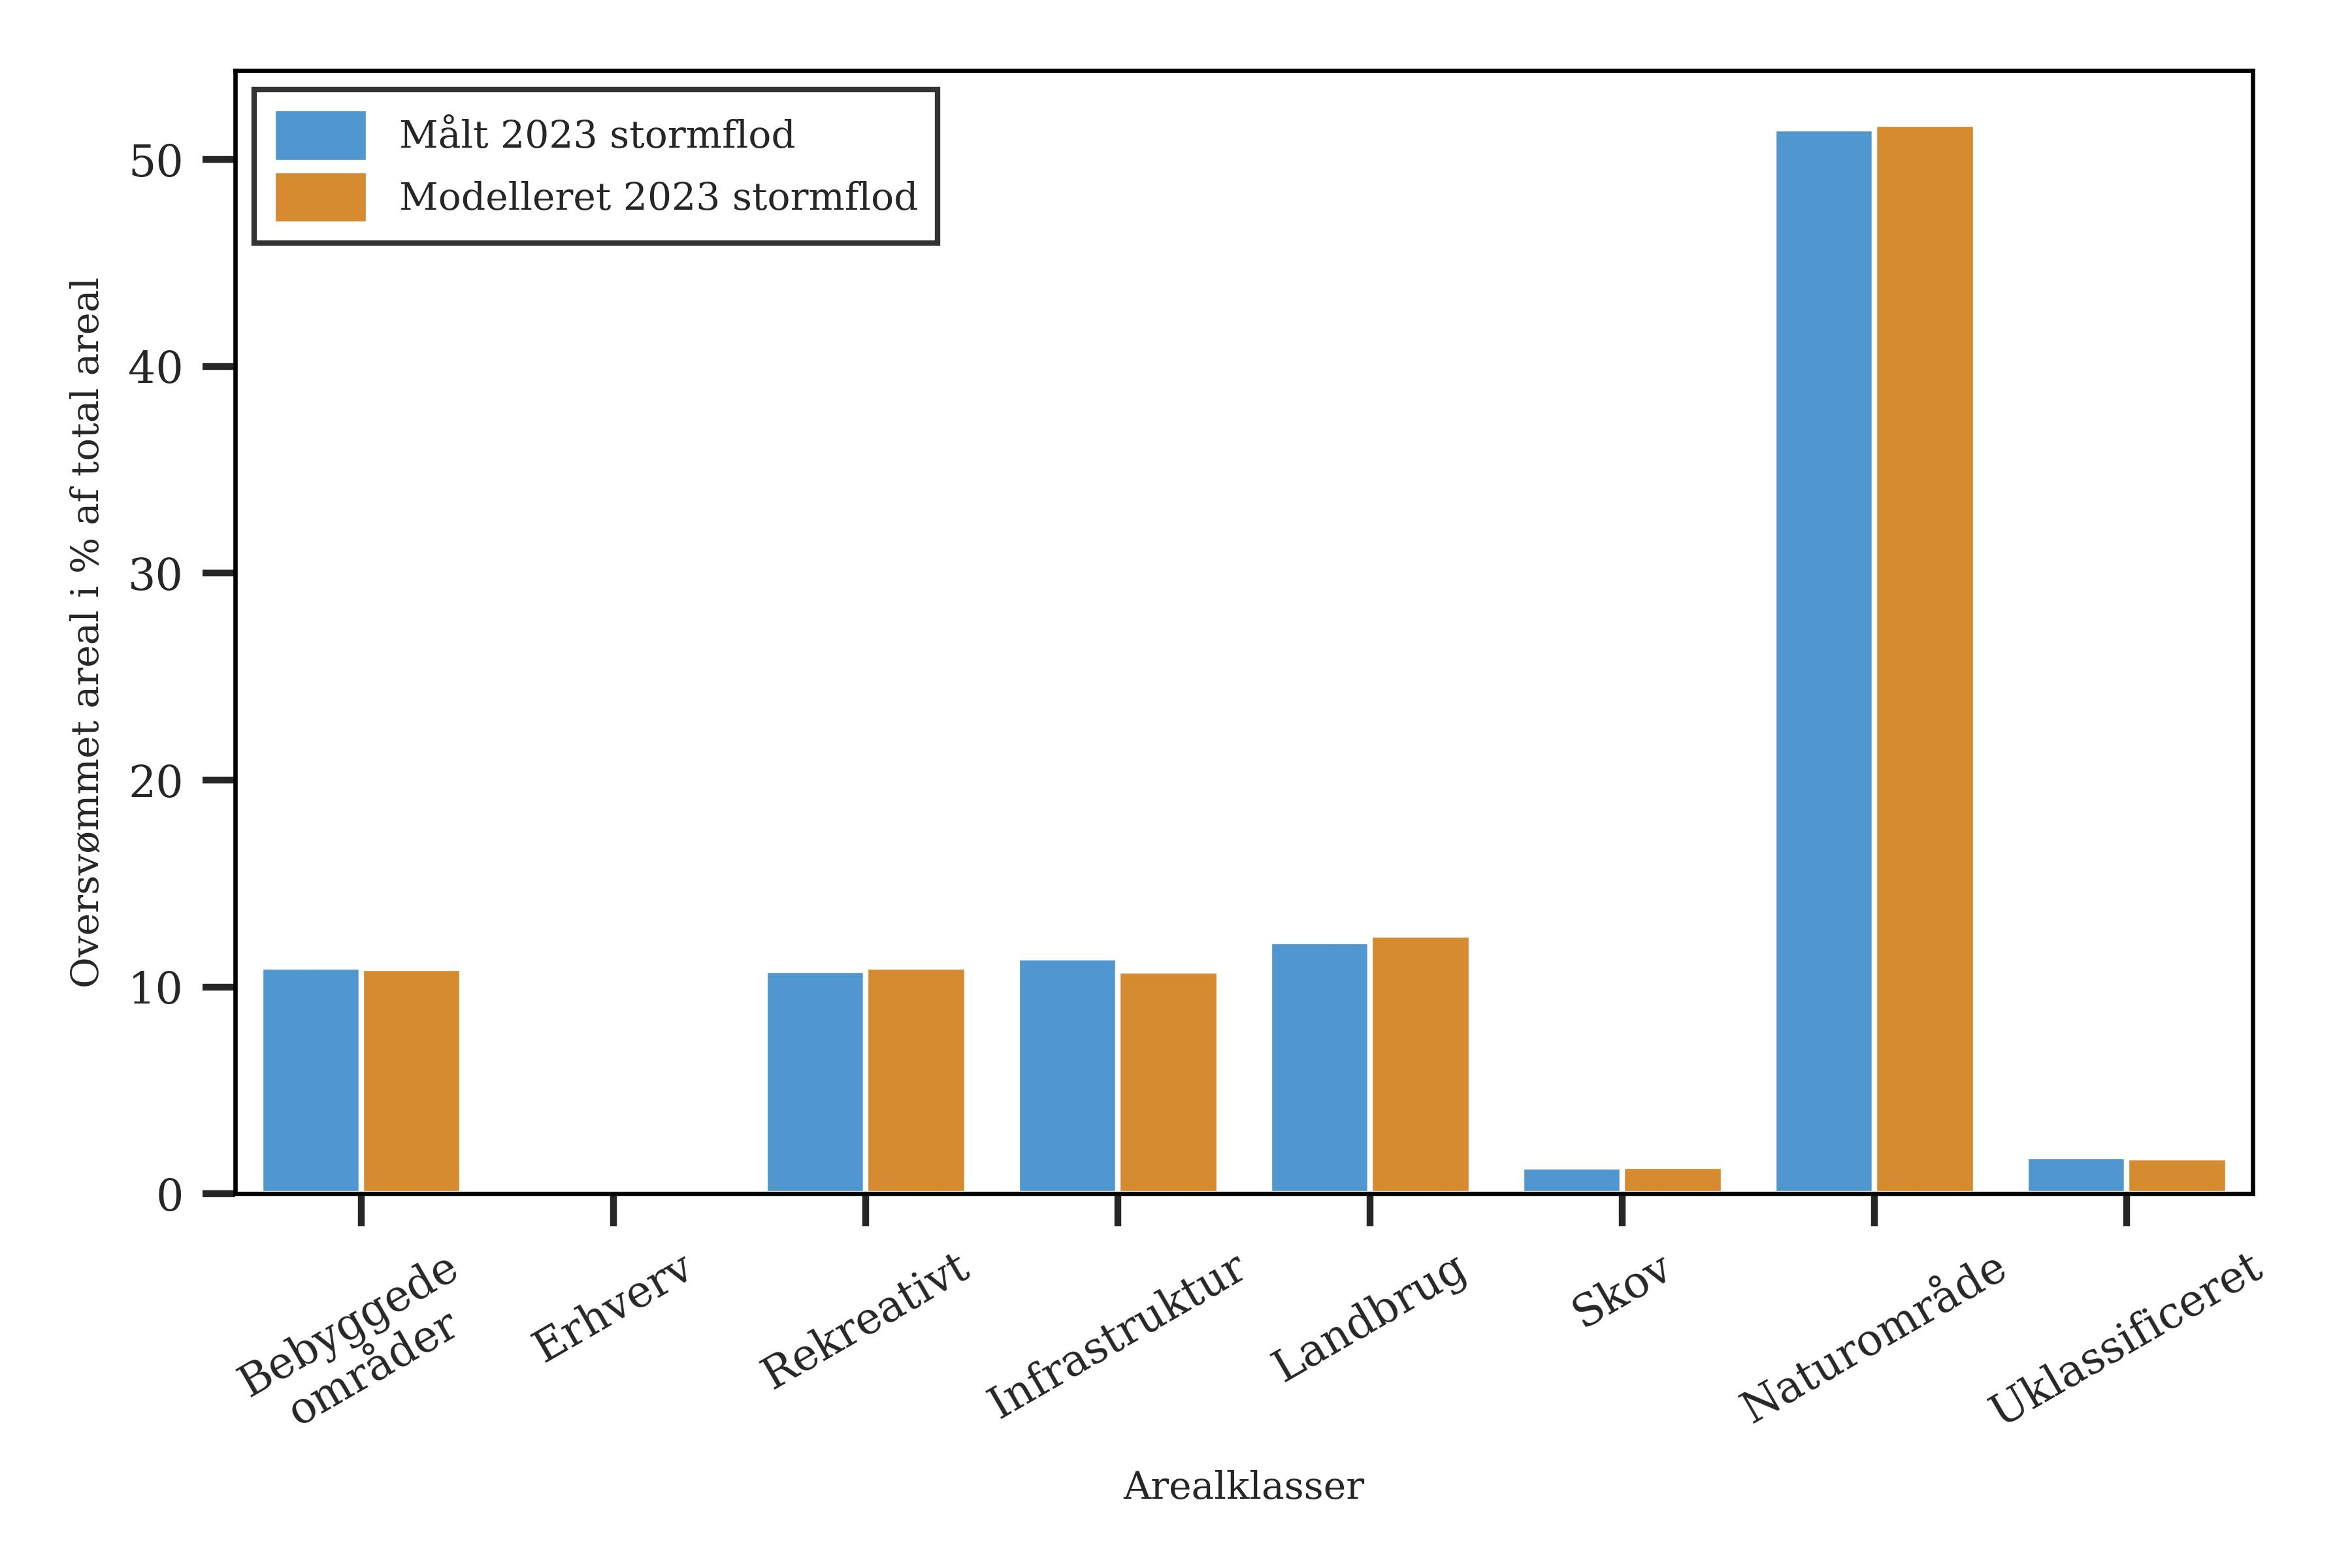
\includegraphics[width=1\linewidth]{images/Resultater/areal_anvendelses_grafer/gedser_arealanvendelse.jpg}
        \caption{}
        \label{Subfig: Procent areal Gedser}
    \end{subfigure}
    \begin{subfigure}[b]{0.5\textwidth}
        \centering
        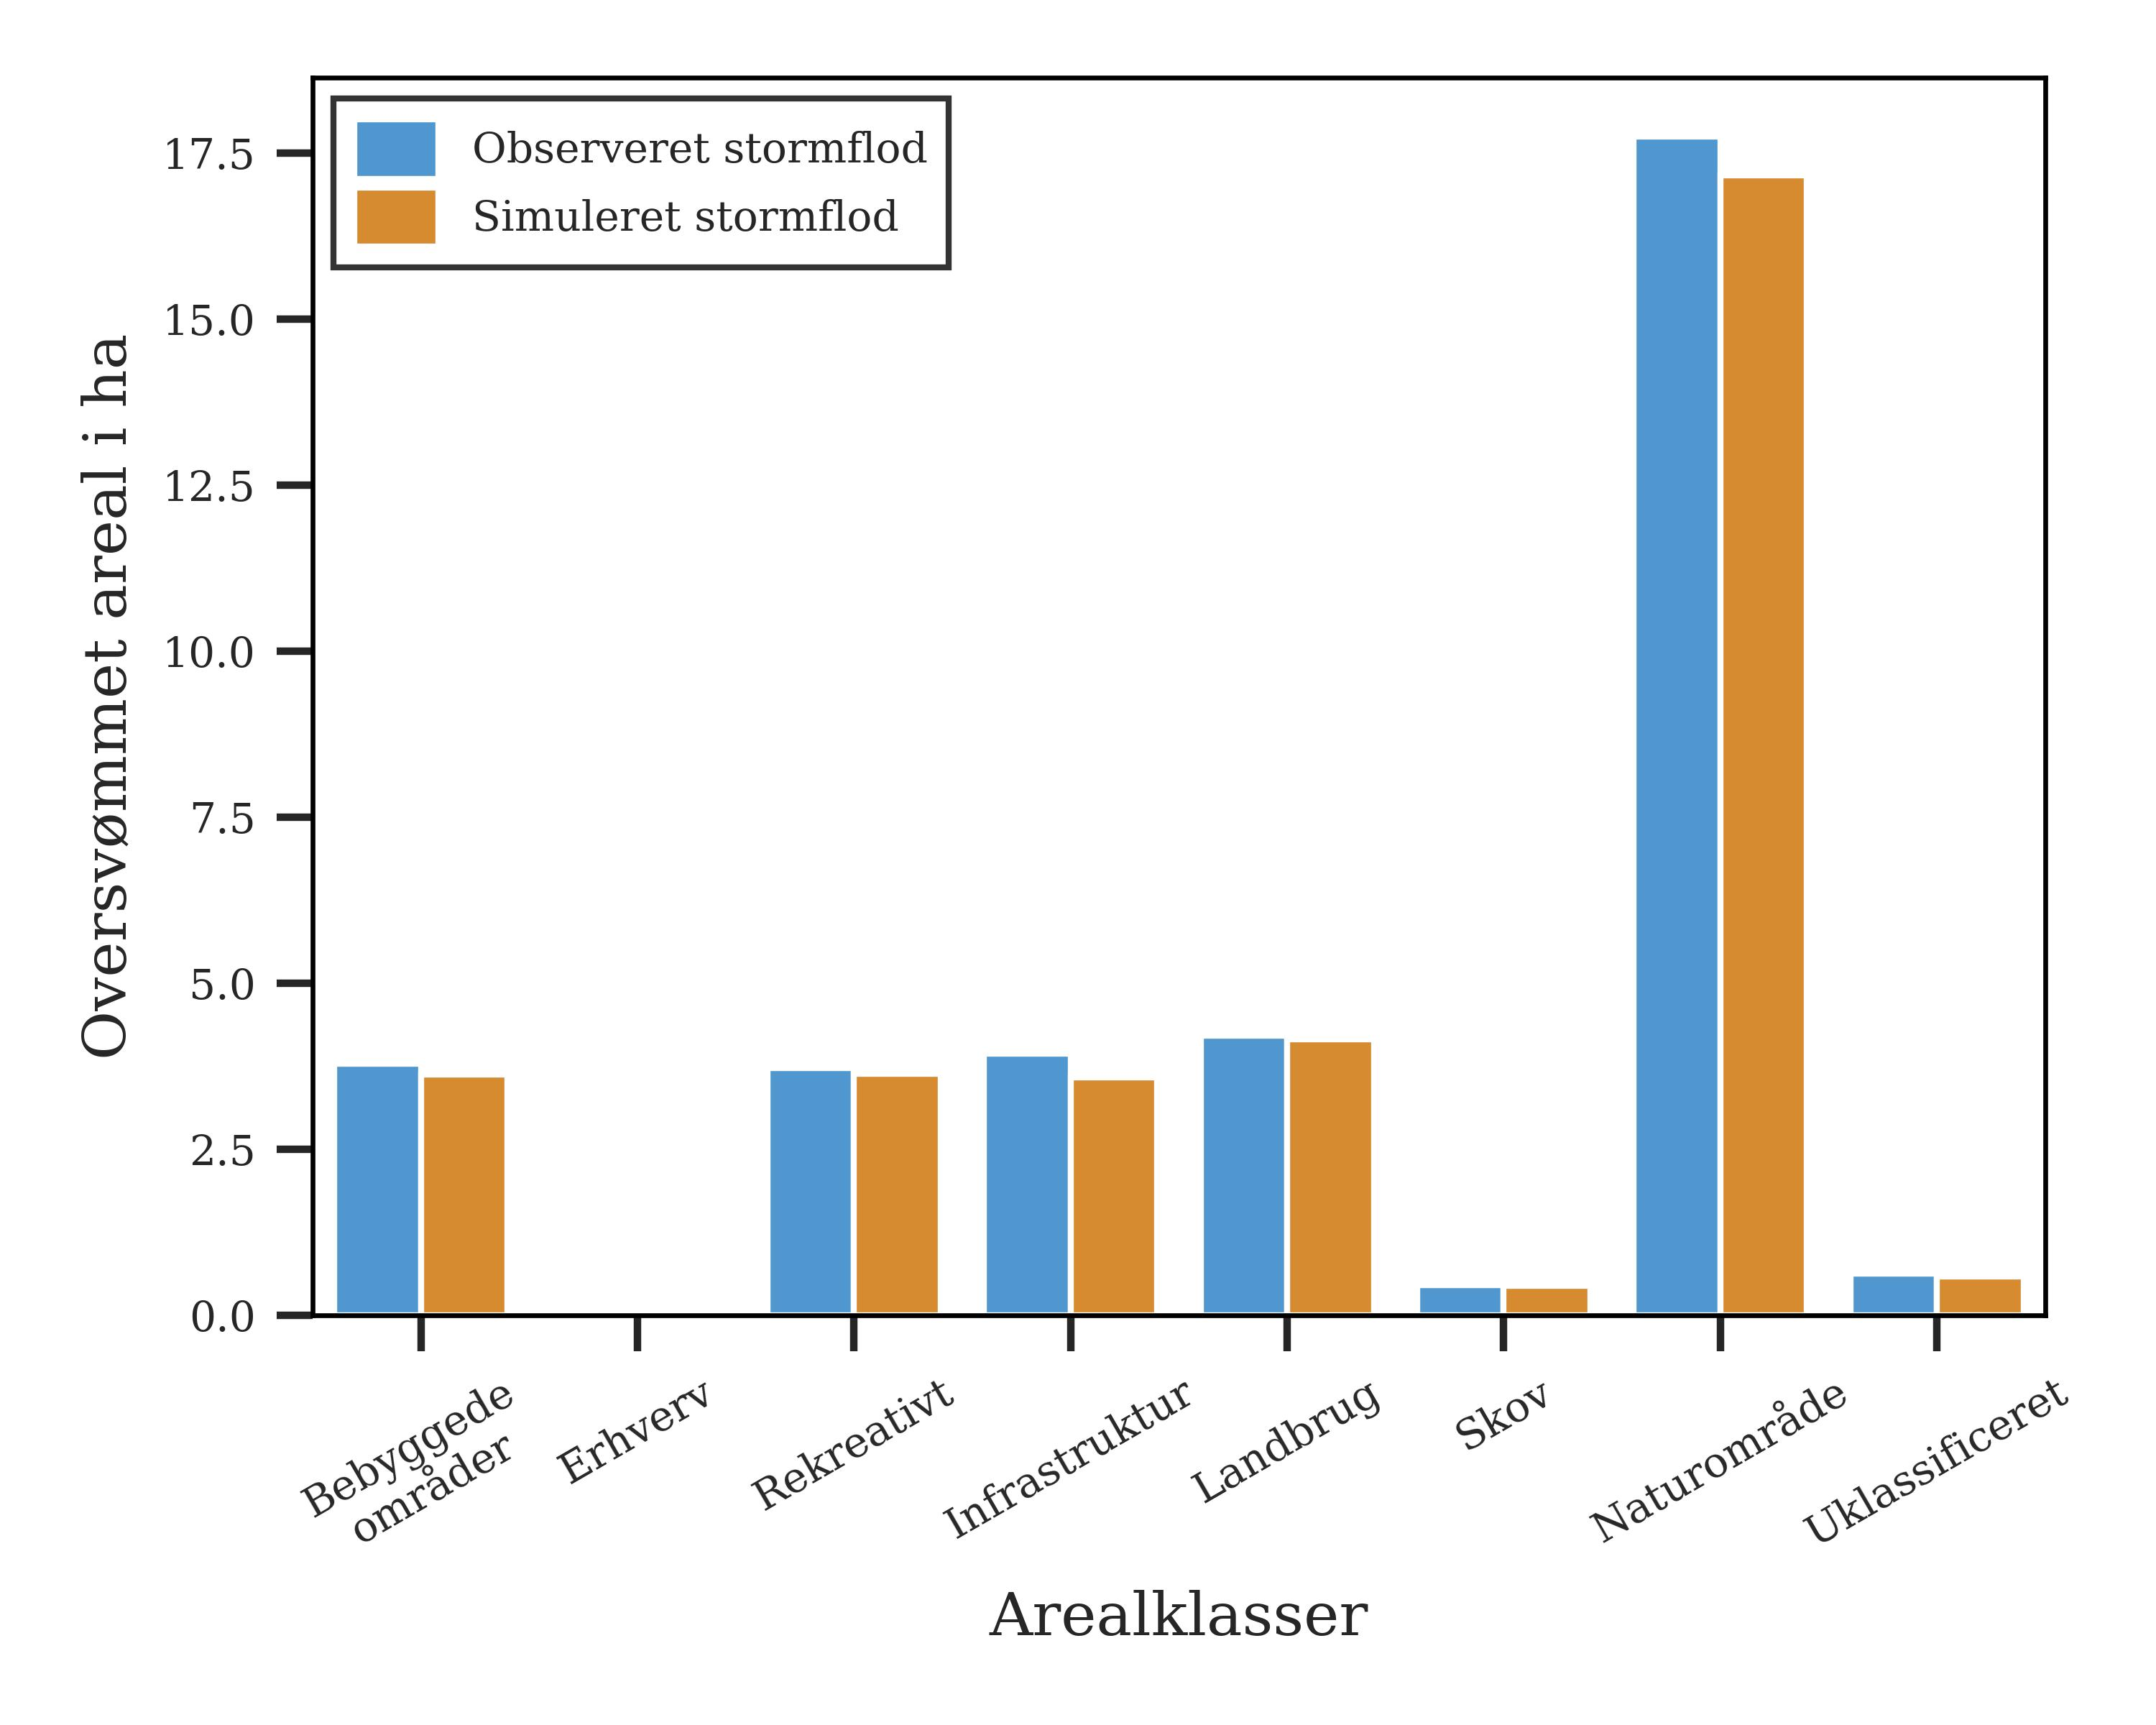
\includegraphics[width=1\linewidth]{images/Resultater/areal_anvendelses_grafer/gedser_oversvommet_Hektar.jpg}
        \caption{}
        \label{Subfig: Hektar areal Gedser}
    \end{subfigure}
    \caption{Påvirkede arealanvendelsesklasser i Gedser Havn for den observeret og simuleret stormflod. Bemærk at kategorien "Erhverv" udgør >0,05\% og er derfor ikke synlig. \textbf{(a)} Oversømmet areal som procent af det totale areal. \textbf{(b)} Oversvømmet areal i hektar.}
    \label{Figur: Påvirket arealanvendelse Gedser}
\end{figure}

For Hesnæs var det primært havnen og kystlinjen der blev oversvømmet under stormfloden (figur \ref{Subfig: Målt Hesnæs}). Resultatet fra Inundation Modellen i figur \ref{Subfig: Model Hesnæs} giver det samme resultat og der er ikke forskel mellem observeret og simuleret resultat. Den observeret hændelse havde et totalt oversvømmet areal på 34,6 ha og det simulerede resultat havde et areal på 33 ha. Modellens resultat er derfor 0,17 ha mindre, svarende til en forskel på 5,2\%.
\begin{figure}[H]
    \begin{subfigure}[t]{0.5\textwidth}
        \centering
        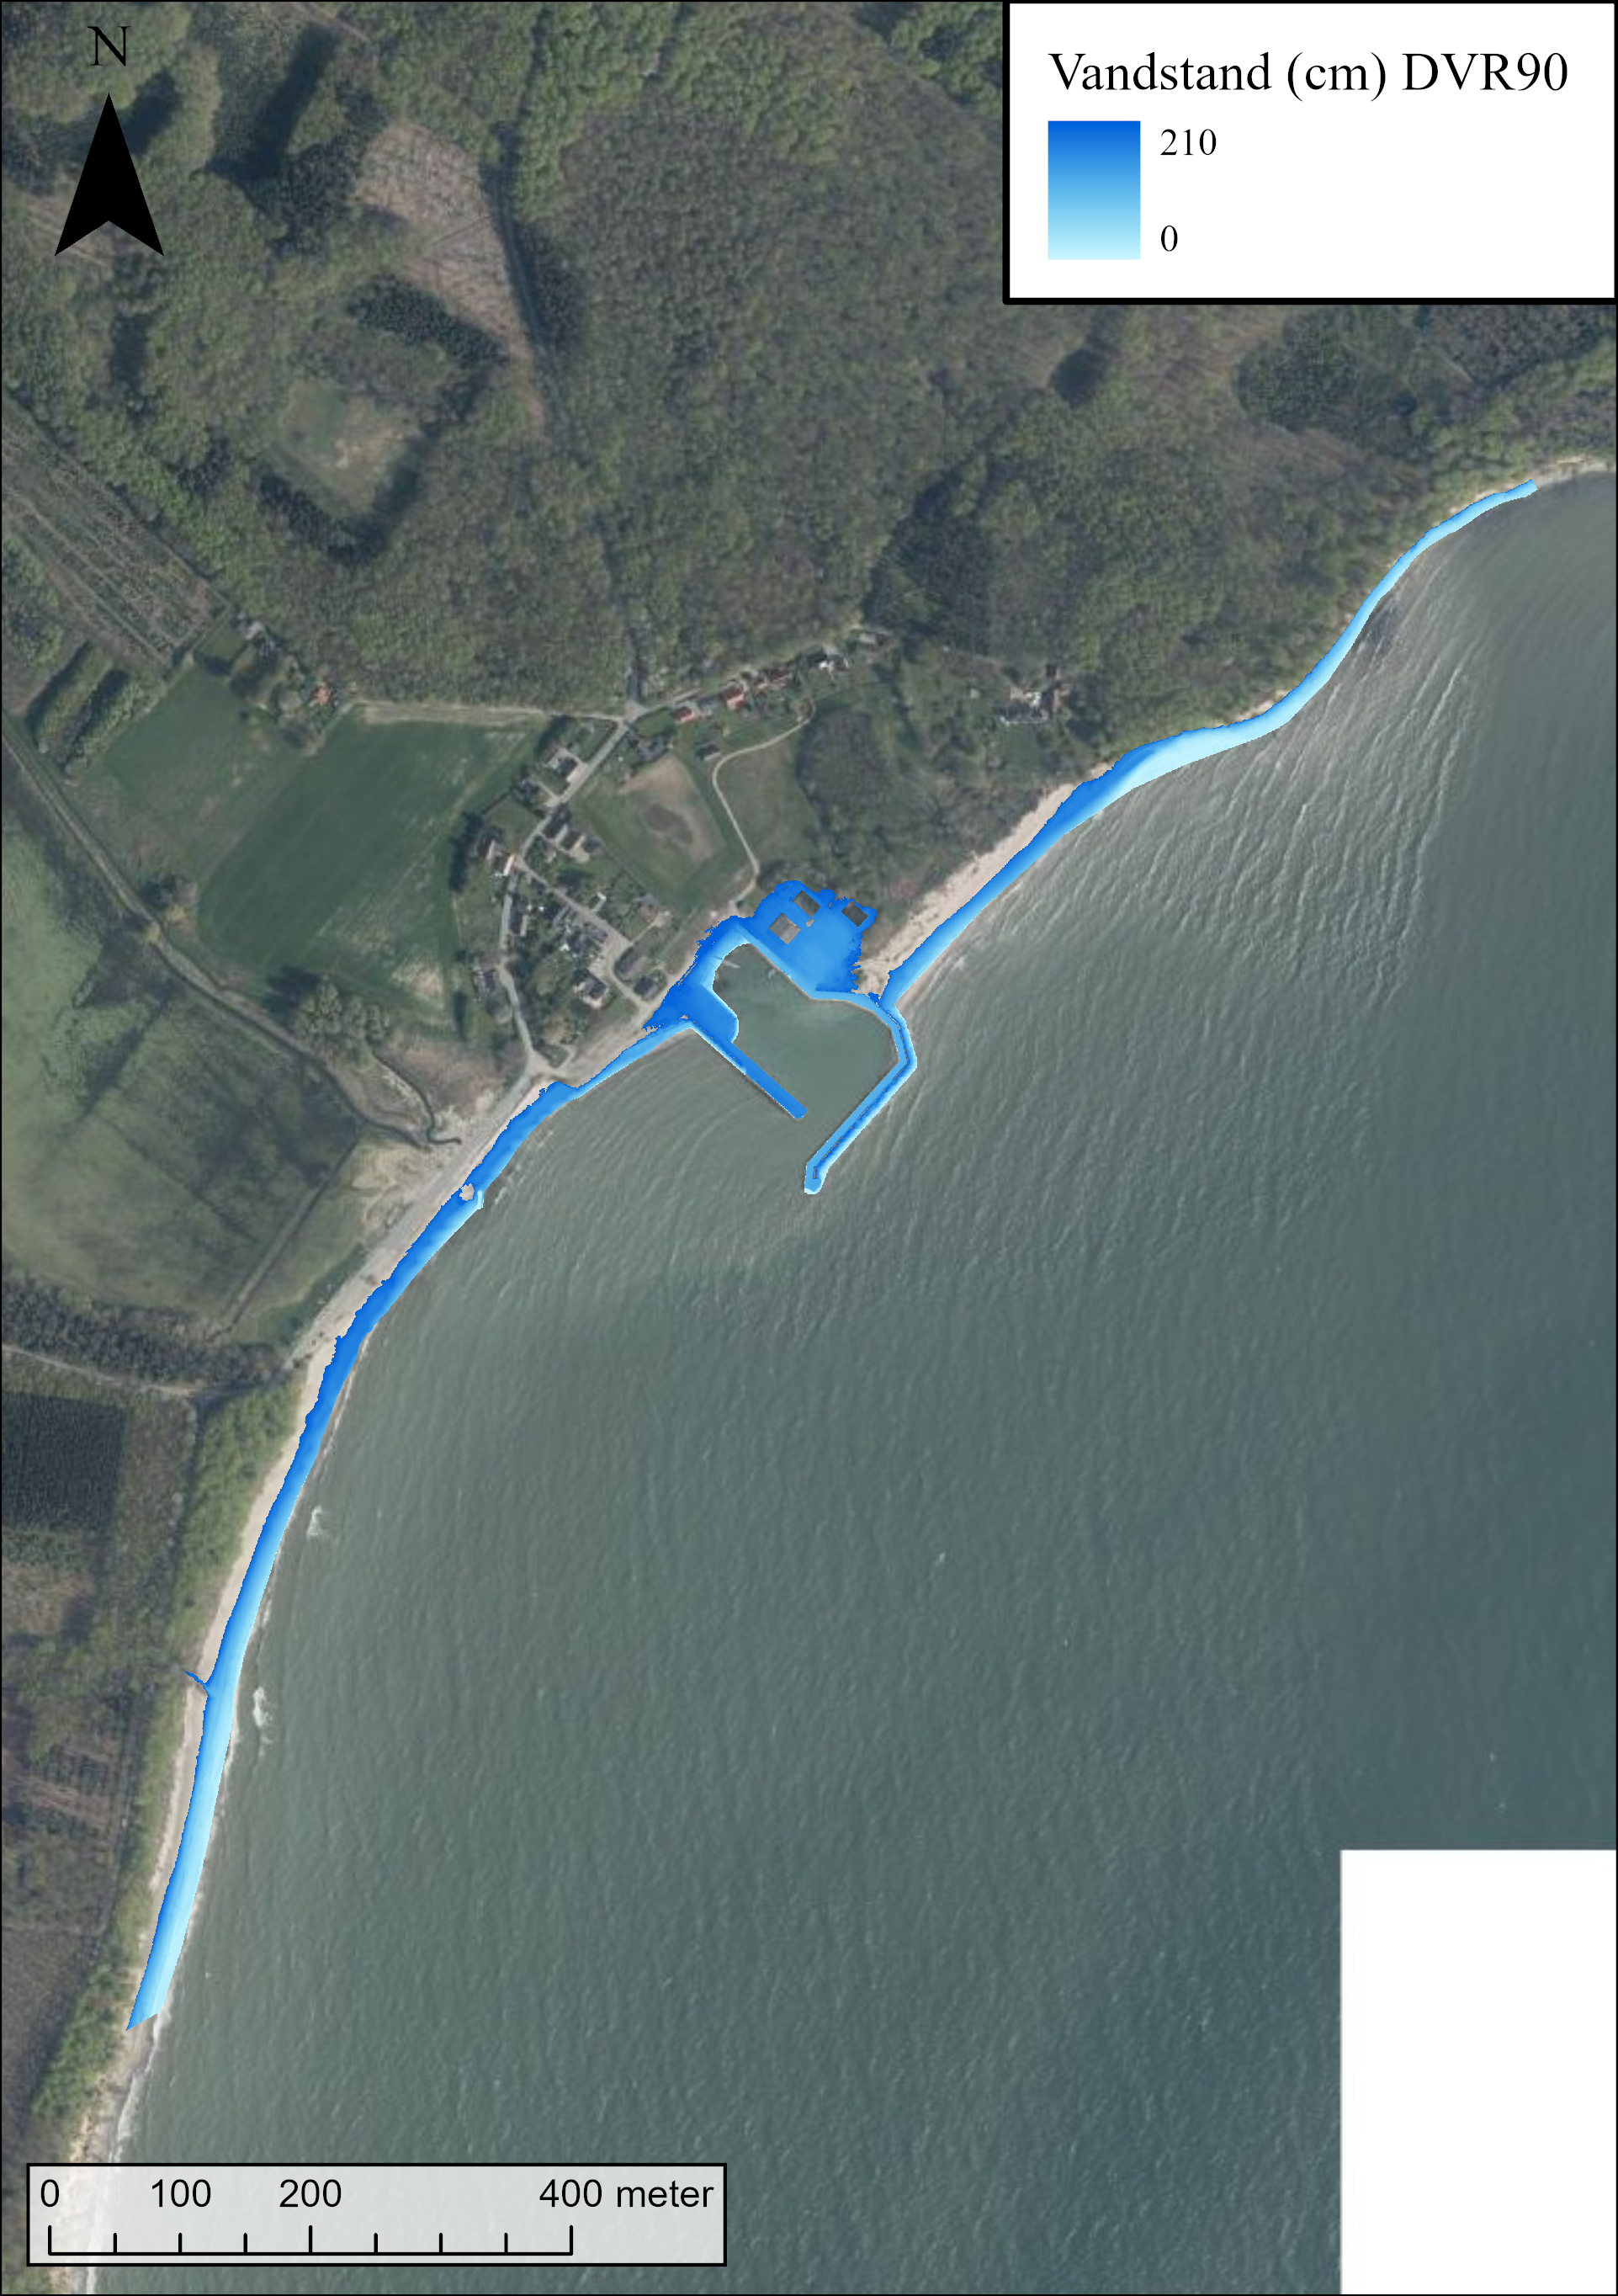
\includegraphics[width=0.95\linewidth]{images/Resultater/2023Malt/2023 resultat_hesnaes.jpg}
        \caption{}
        \label{Subfig: Målt Hesnæs}
    \end{subfigure}
    \begin{subfigure}[t]{0.5\textwidth}
        \centering
        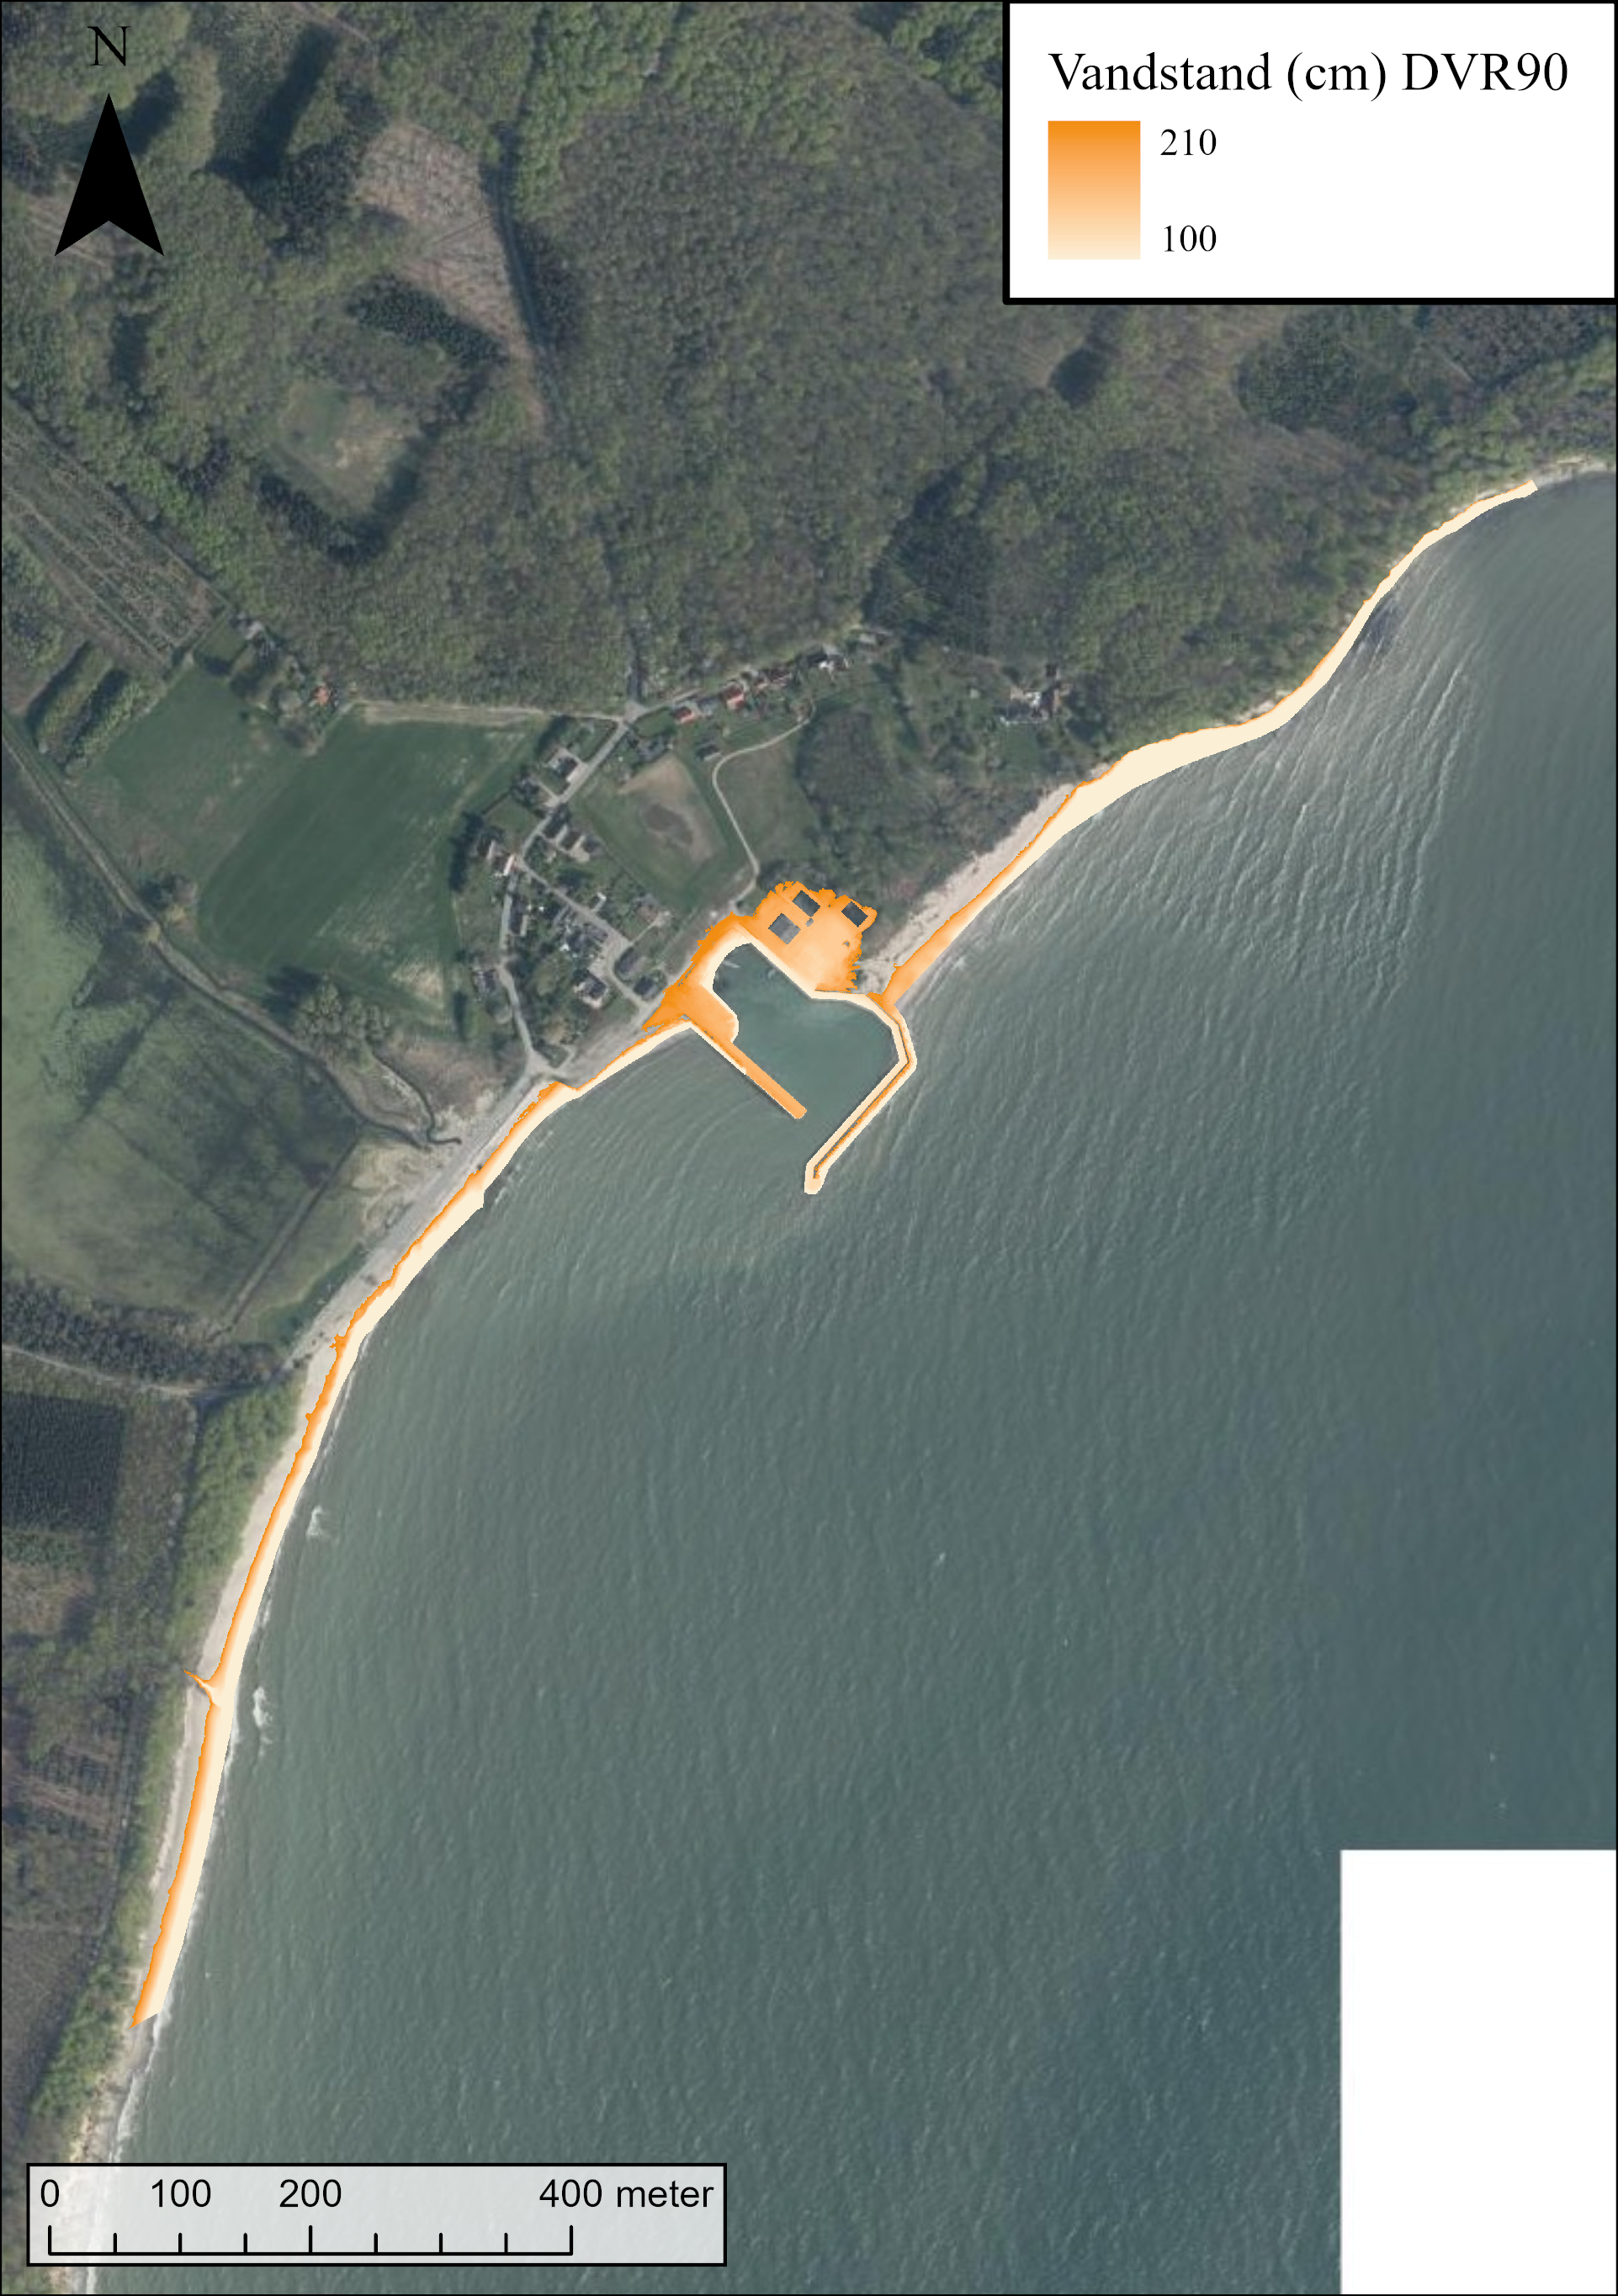
\includegraphics[width=0.95\linewidth]{images/Resultater/2023Model/2023 model_hesnaes.jpg}
        \caption{}
        \label{Subfig: Model Hesnæs}
    \end{subfigure}
    \caption{Oversvømmelseskort over oktober 2023 stormfloden for Hesnæs. \textbf{(a)} Observeret data. \textbf{(b)} Simuleret data.}
    \label{Figur: Målt & simuleret Hesnæs}
\end{figure} 

I Hesnæs blev seks forskellige arealanvendelser påvirket. De mest påvirkede arealer i Hesnæs var kysten, der falder ind under naturområder. Dette har været gældende for begge resultater. For den observeret hændelse blev 66,2\% naturområde oversvømmet og for den simuleret hændelse blev 65,8\% oversvømmet (figur \ref{Subfig: Procent hesnæs}). Dette svarer til henholdsvis 2,3 og 2,2 ha (figur \ref{Subfig: Hektar Hesnæs}). For de andre arealklasser er resultatet ens for den observeret og simuleret stormflod. 
\begin{figure}[H]
    \begin{subfigure}[b]{0.5\textwidth}
        \centering
        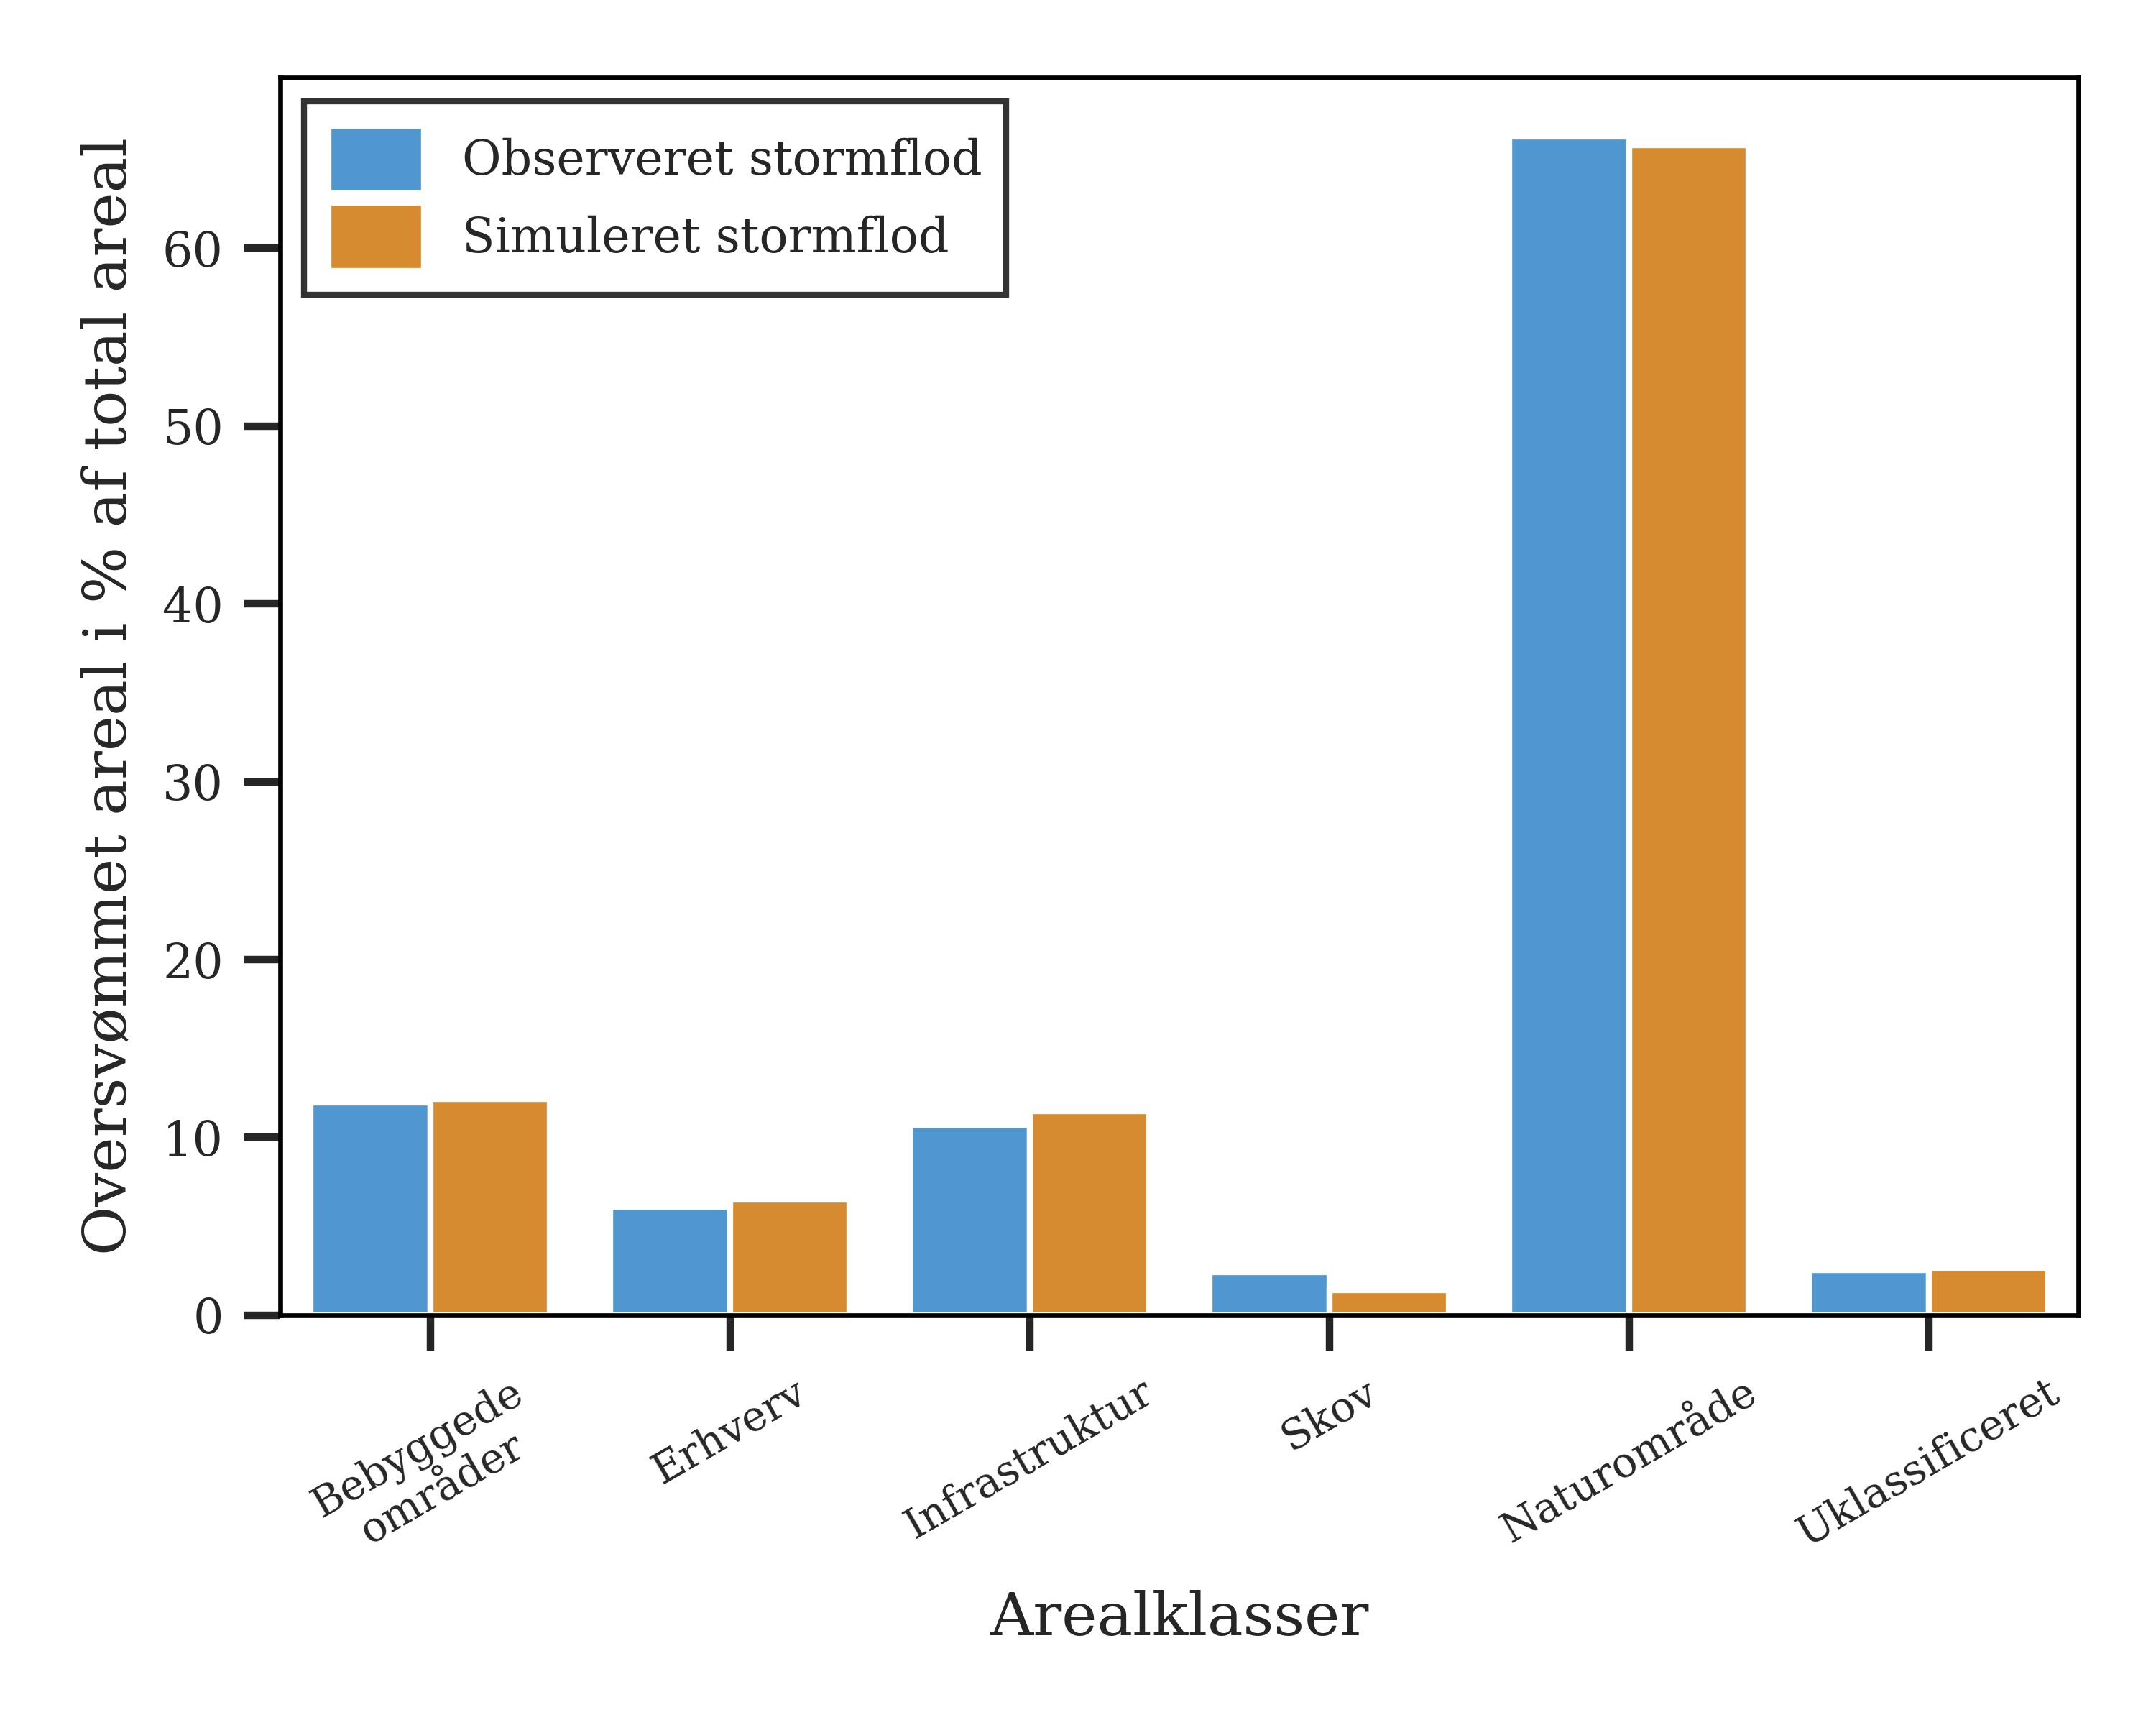
\includegraphics[width=1\linewidth]{images/Resultater/areal_anvendelses_grafer/hesnaes_arealanvendelse.jpg}
        \caption{}
        \label{Subfig: Procent hesnæs}
    \end{subfigure}
    \begin{subfigure}[b]{0.5\textwidth}
        \centering
        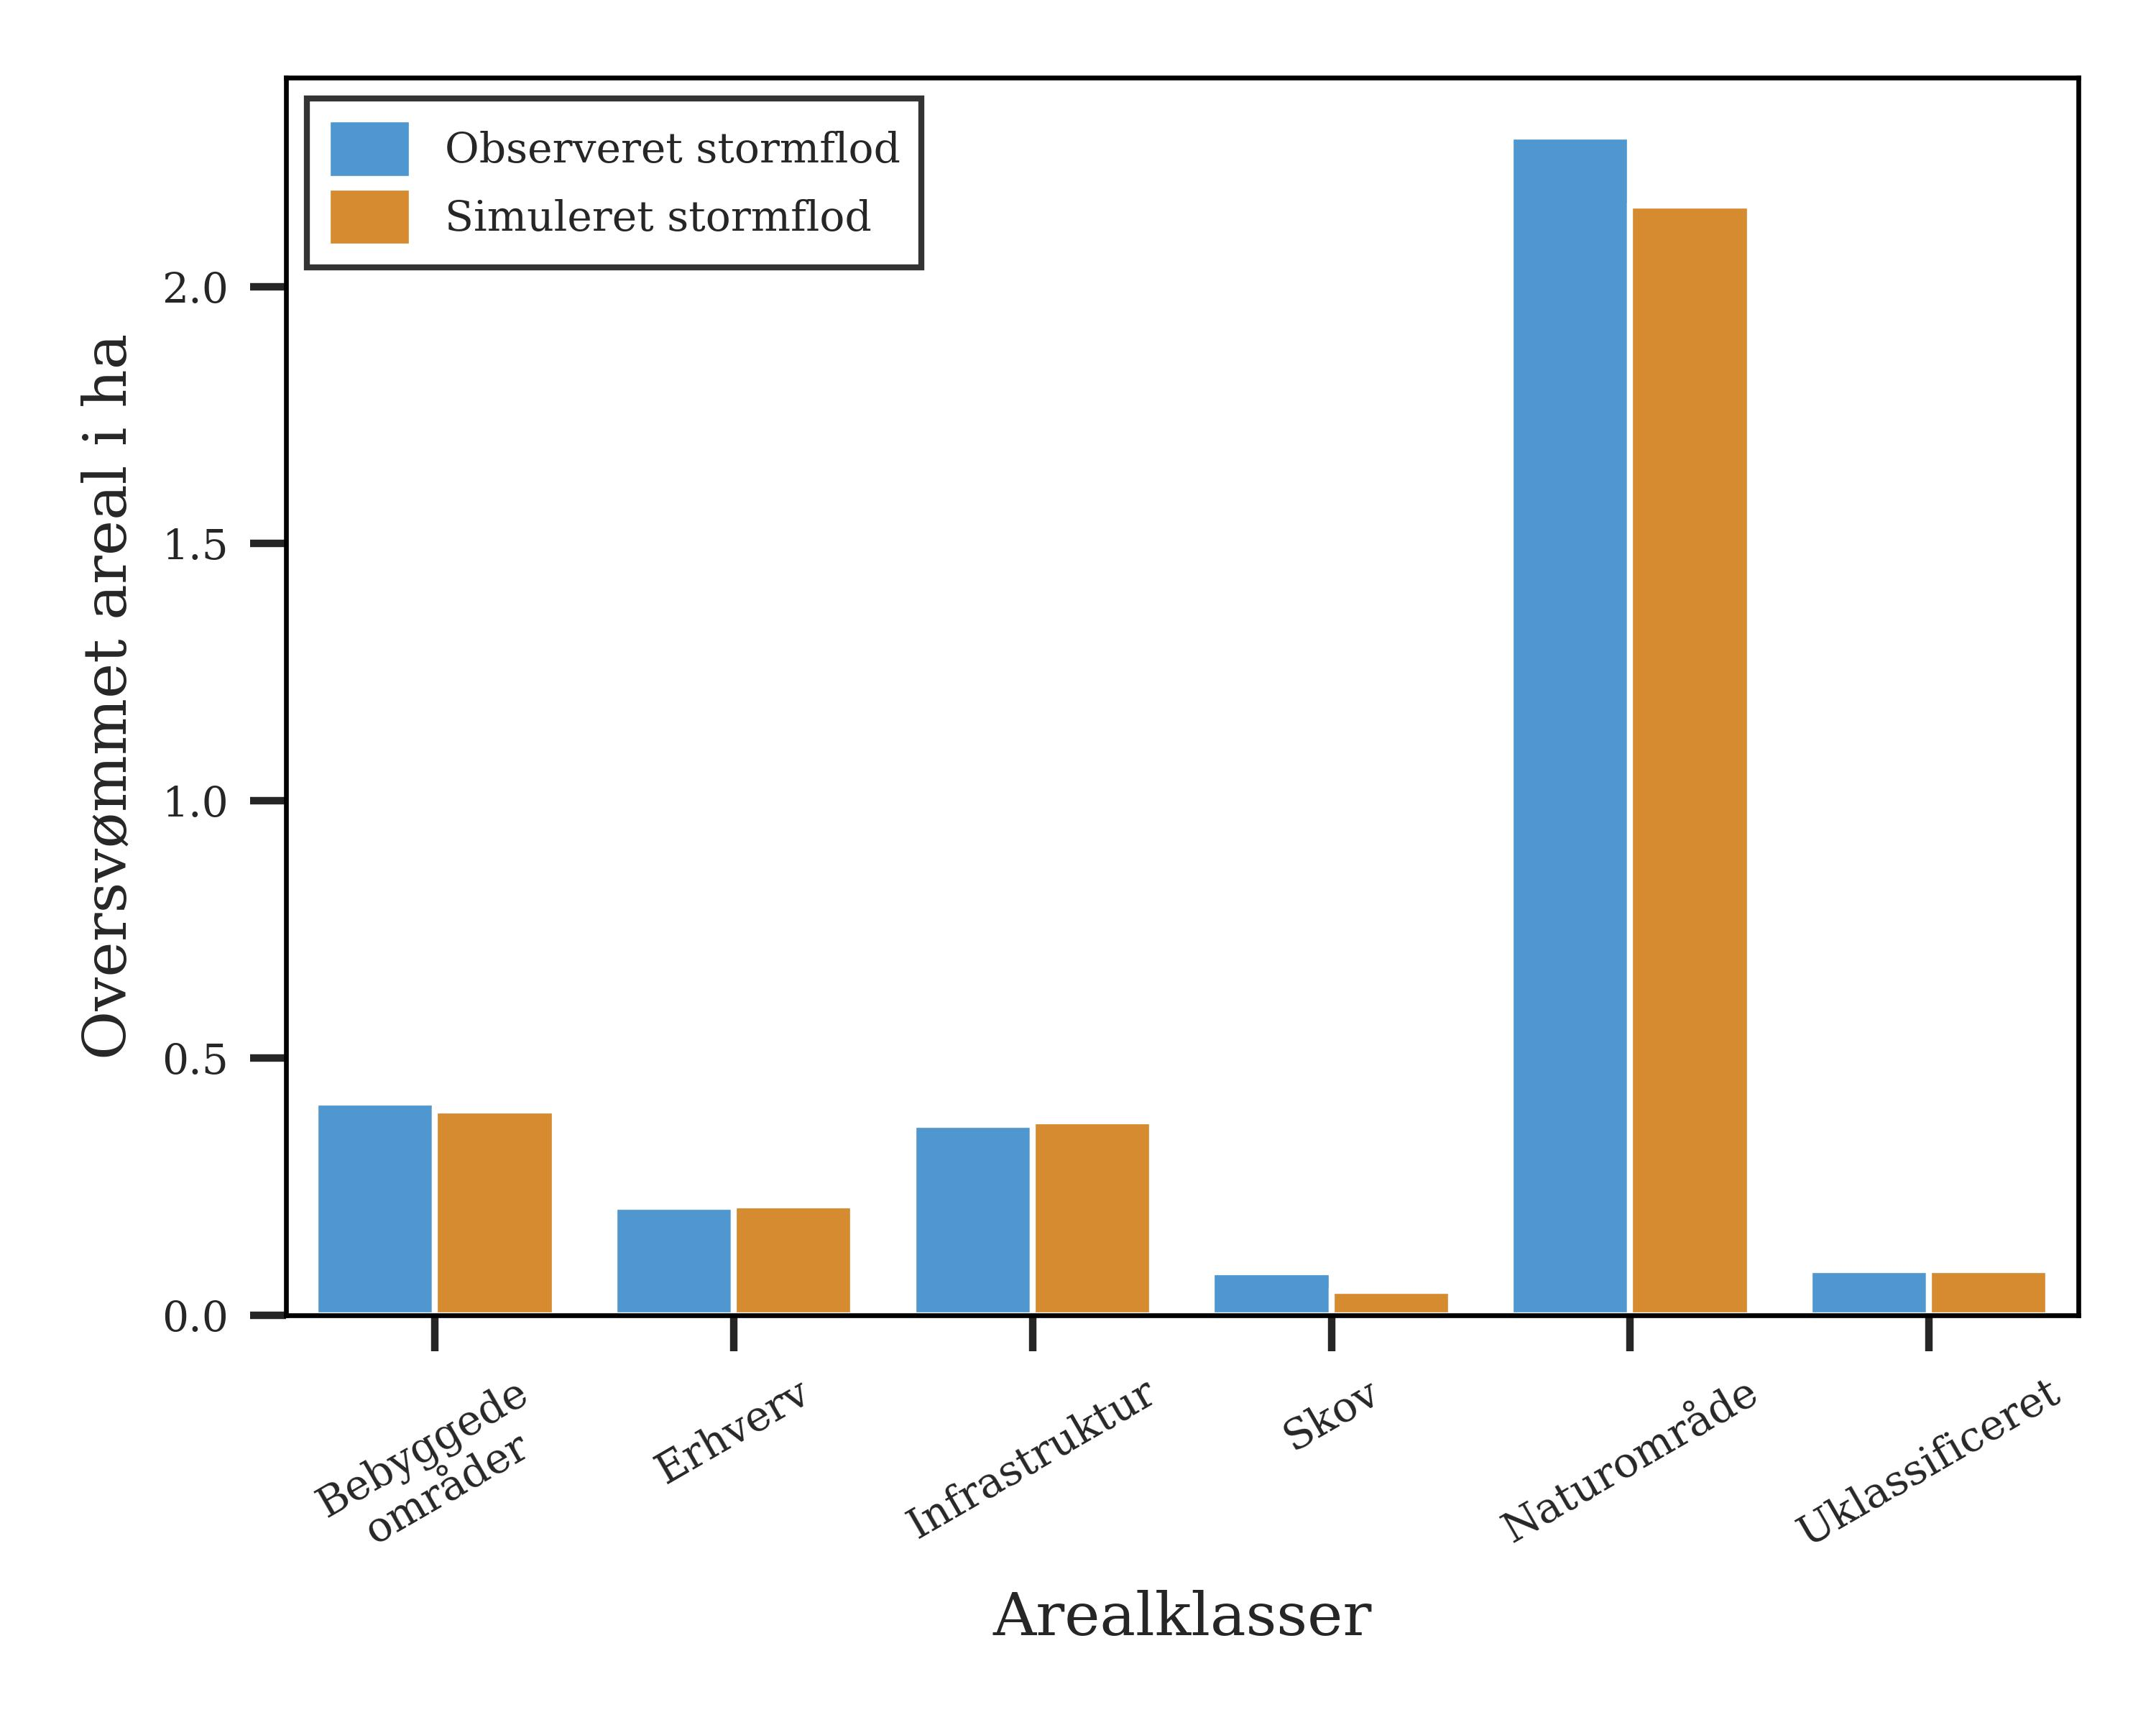
\includegraphics[width=1\linewidth]{images/Resultater/areal_anvendelses_grafer/hesnaes_oversvommet_Hektar.jpg}
        \caption{}
        \label{Subfig: Hektar Hesnæs}
    \end{subfigure}
    \caption{Påvirkede arealanvendelsesklasser i Hesnæs for den observeret og simuleret stormflod. \textbf{(a)} Oversømmet areal som procent af det totale areal. \textbf{(b)} Oversvømmet areal i hektar.}
    \label{Figur: Påvirket arealanvendelse Hesnæs}
\end{figure}


Figur \ref{Figur: Målt & simuleret Præstø} viser den observeret stormflods hændelse og den simuleret hændelse i Præstø. Begge kort viser at kysten og havnen af Præstø bliver oversvømmet samt den nordlige bydel. Den største forskel mellem de to oversvømmelseskort er at den observeret hændelse blev en del af Tubæk Ådal oversvømmet. Den observeret hændelse på 53,5 ha er derfor 26\% større i udbredelse end det simuleret resultat på 39.8, som svarer til 13,7 ha. 

\begin{figure}[H]
    \begin{subfigure}[t]{0.5\textwidth}
        \centering
        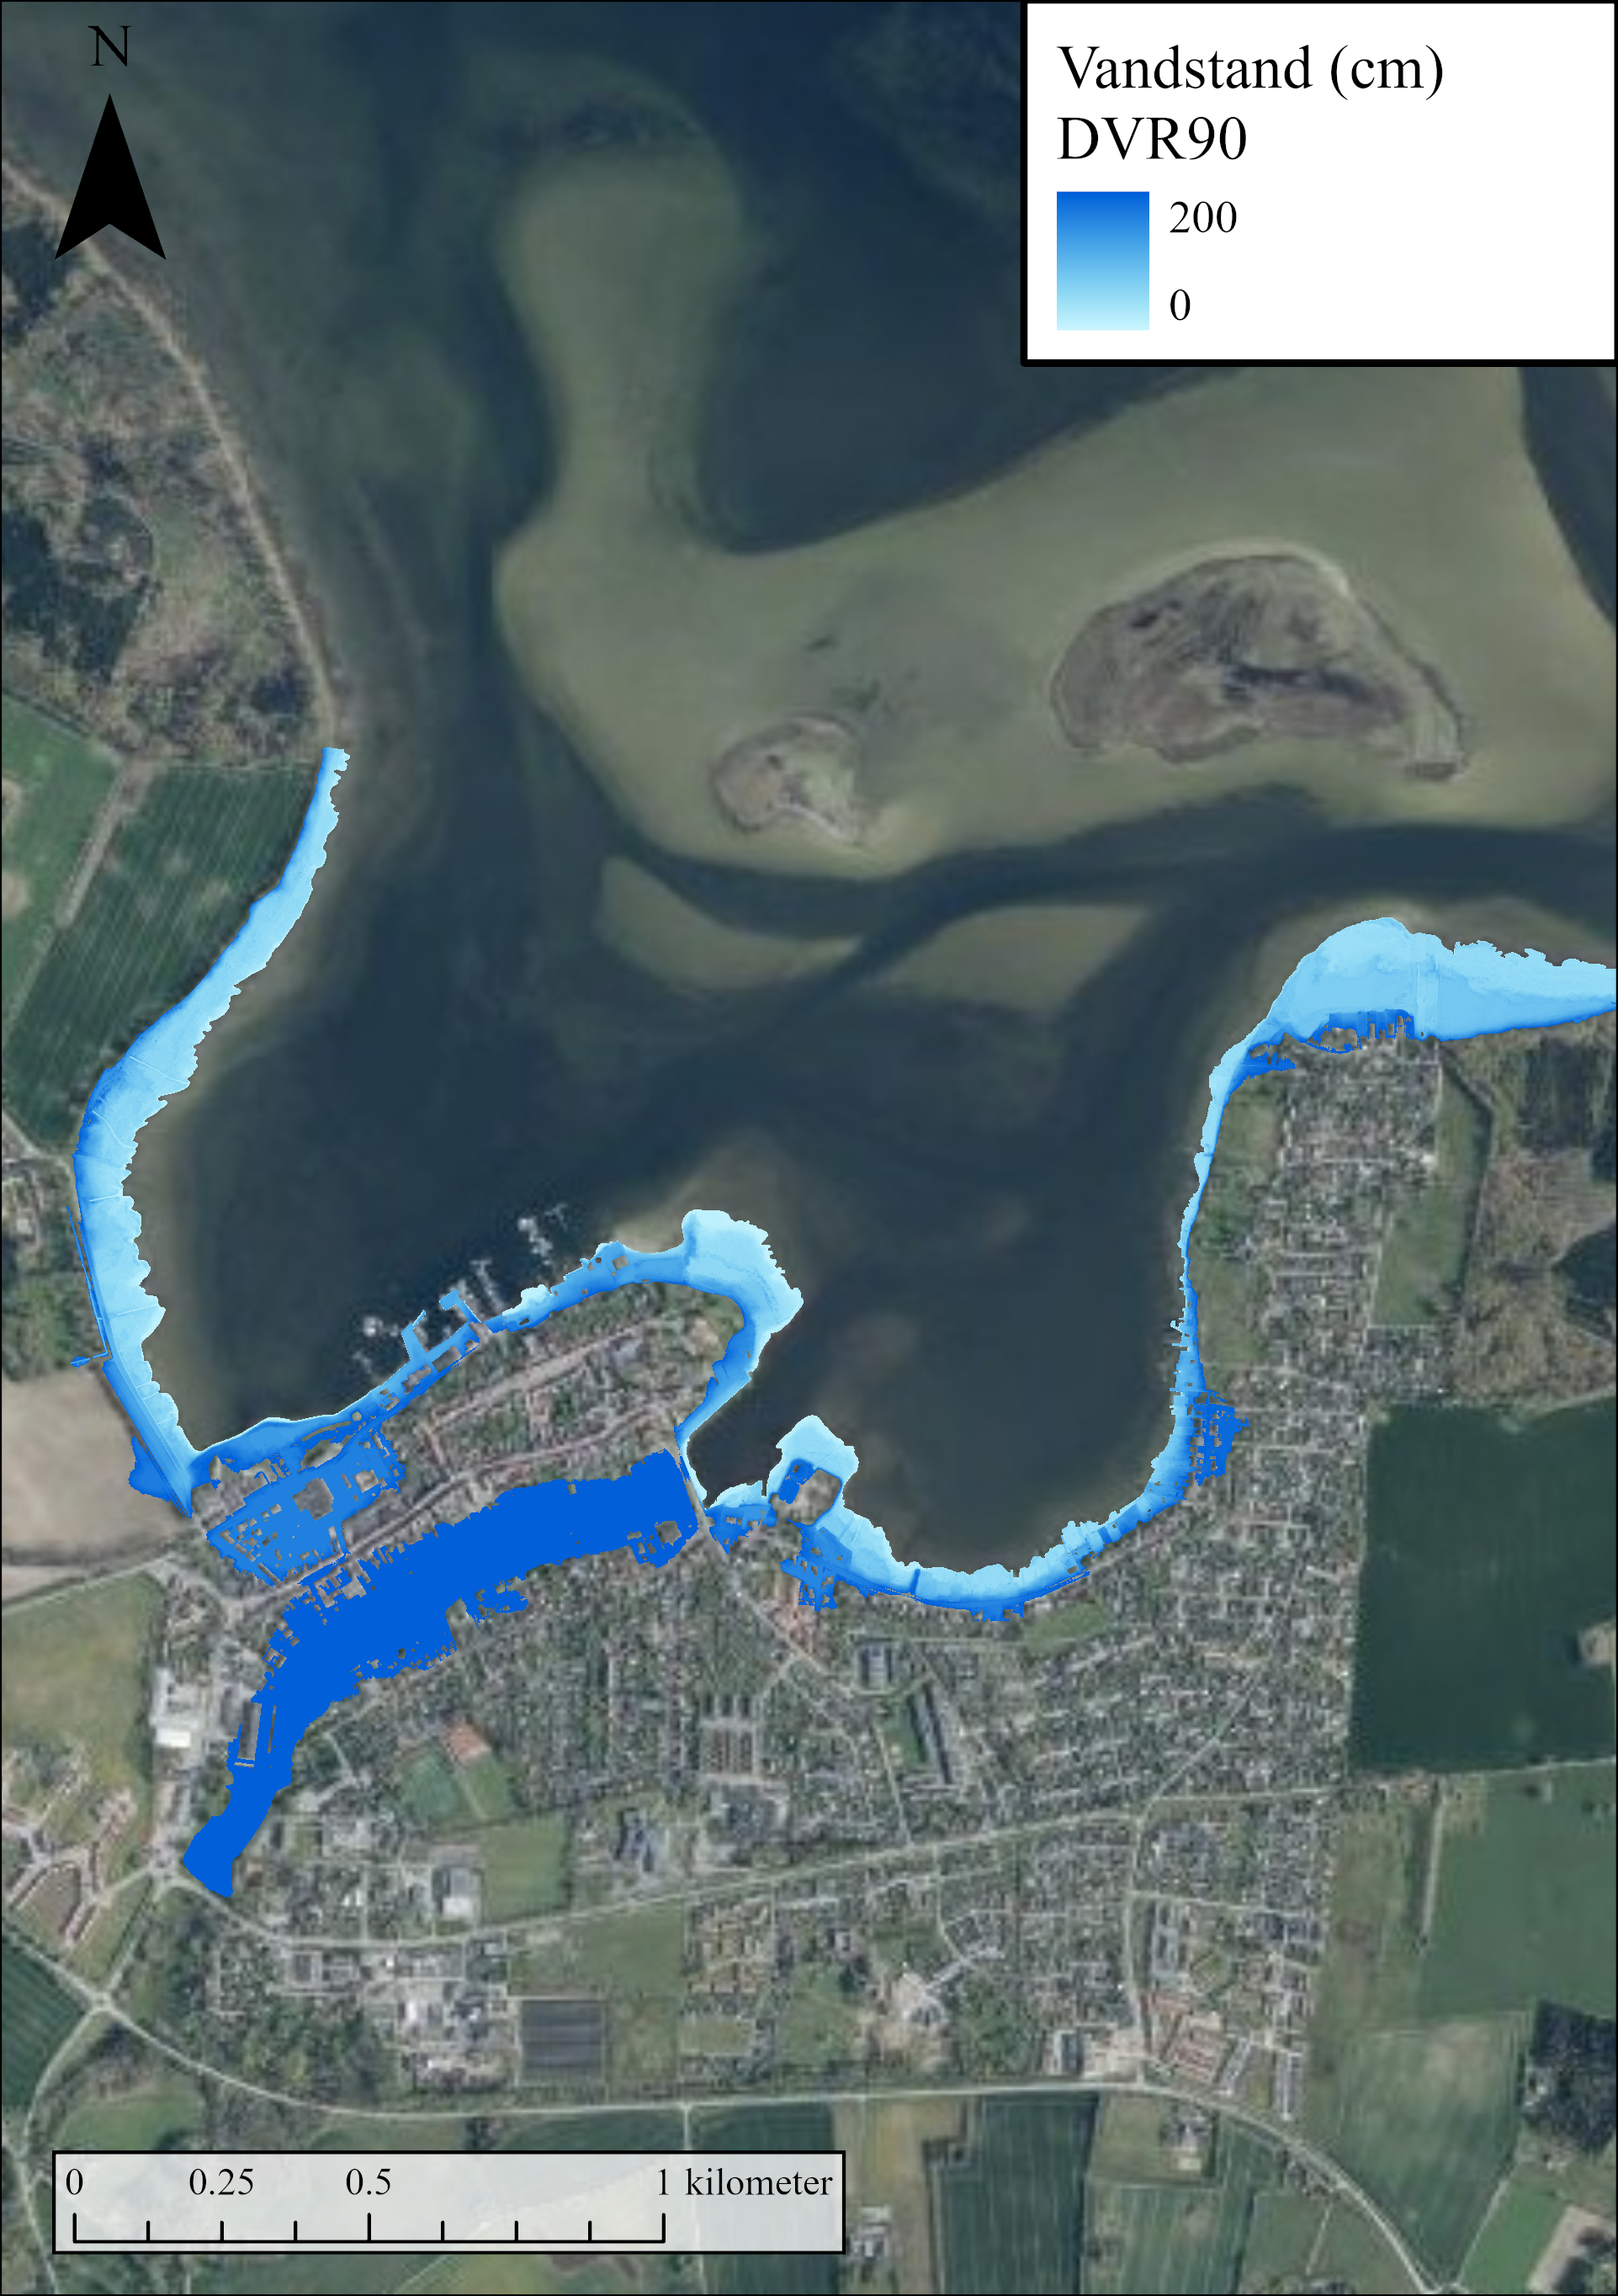
\includegraphics[width=0.95\linewidth]{images/Resultater/2023Malt/2023 resultat_praestoe.jpg}
        \caption{}
        \label{Subfig: Målt Præstø}
    \end{subfigure}
    \begin{subfigure}[t]{0.5\textwidth}
        \centering
        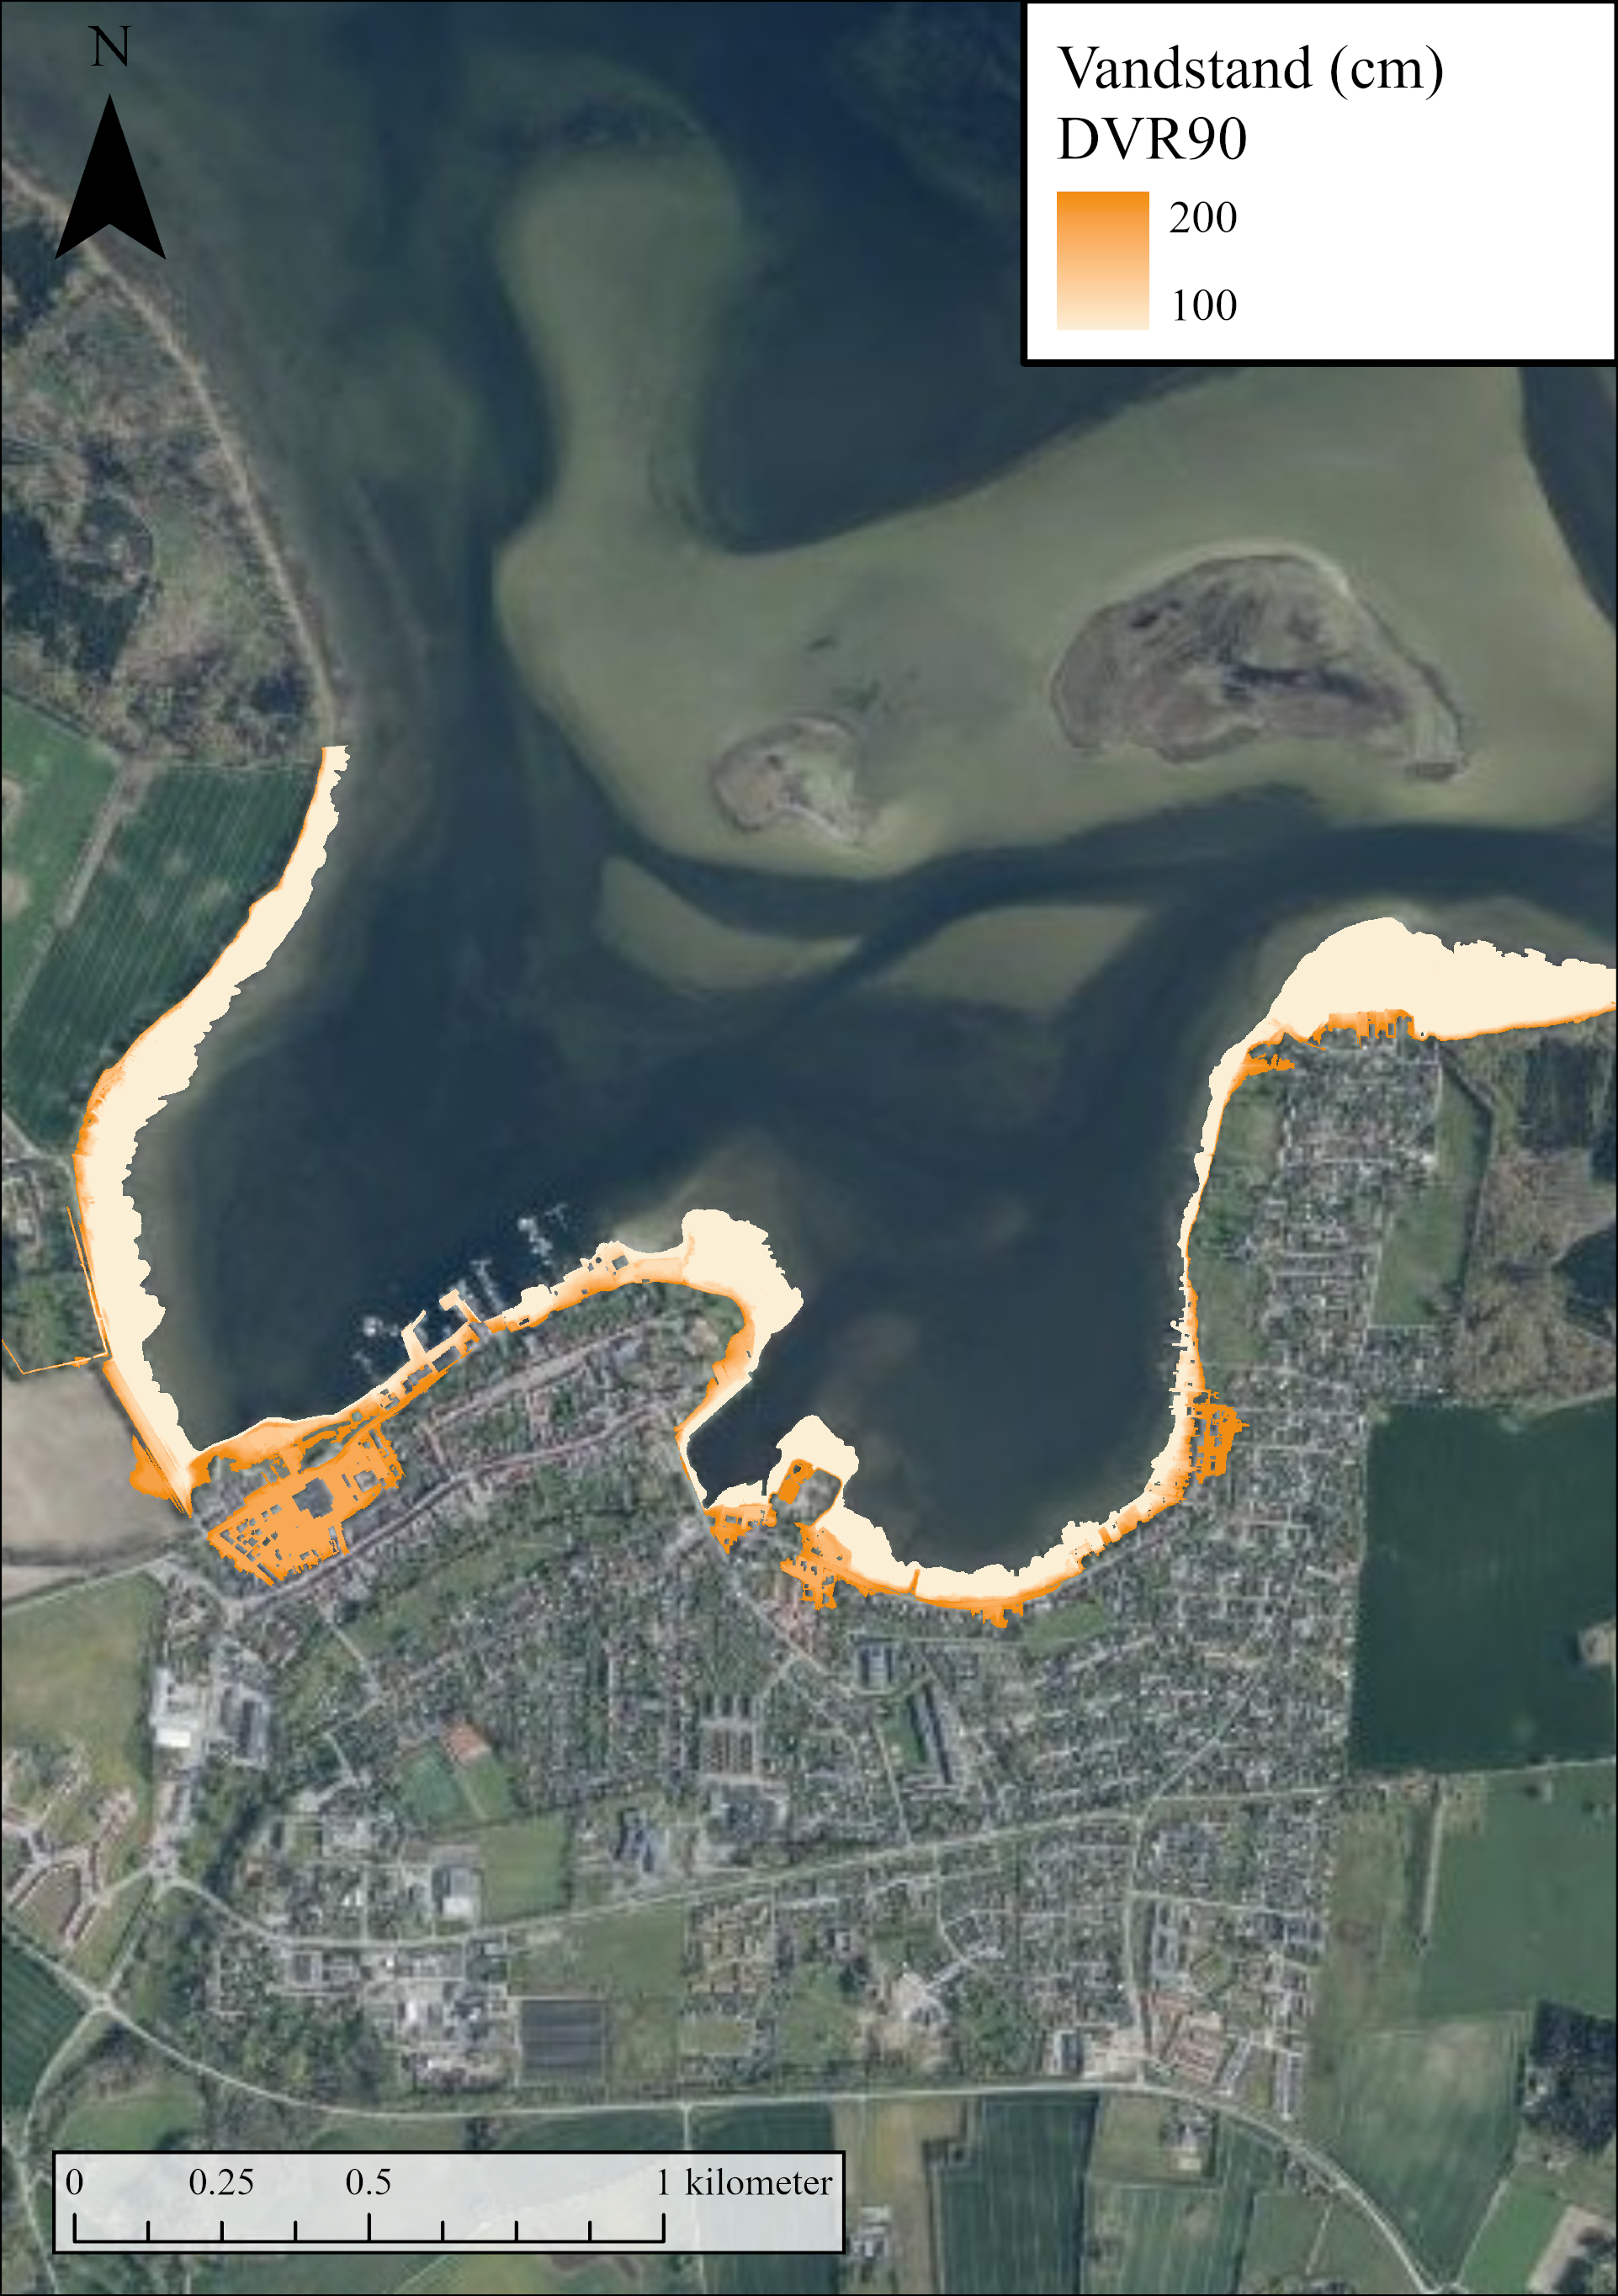
\includegraphics[width=0.95\linewidth]{images/Resultater/2023Model/2023 model_praestoe.jpg}
        \caption{}
        \label{Subfig: Model Præstø}
    \end{subfigure}
    \caption{Oversvømmelseskort over oktober 2023 stormfloden for Præstø. \textbf{(a)} Observeret data. \textbf{(b)} Simuleret data}
    \label{Figur: Målt & simuleret Præstø}
\end{figure}

I Præstø blev otte forskellige arealanvendelser påvirket af stormfloden. For både den observeret og simuleret hændelse var naturområde det mest påvirket areal med 47 og 60\% henholdsvis (figur \ref{Subfig: Procent præstø}). Den observeret hændelse havde et større rekreativt område oversvømmet end den simuleret hændelse med en forskel på 4 ha, da arealerne langs Tubæk Ådal er klassificeret som rekreative områder. Grundet oversvømmelsen af Tubæk Ådal er et større bebygget areal blevet oversvømmet med ca. 12 ha i den observeret stormflod og 6 ha i den simuleret stormflod (figur \ref{Subfig: Hektar præstø}).
\begin{figure}[H]
    \begin{subfigure}[b]{0.5\textwidth}
        \centering
        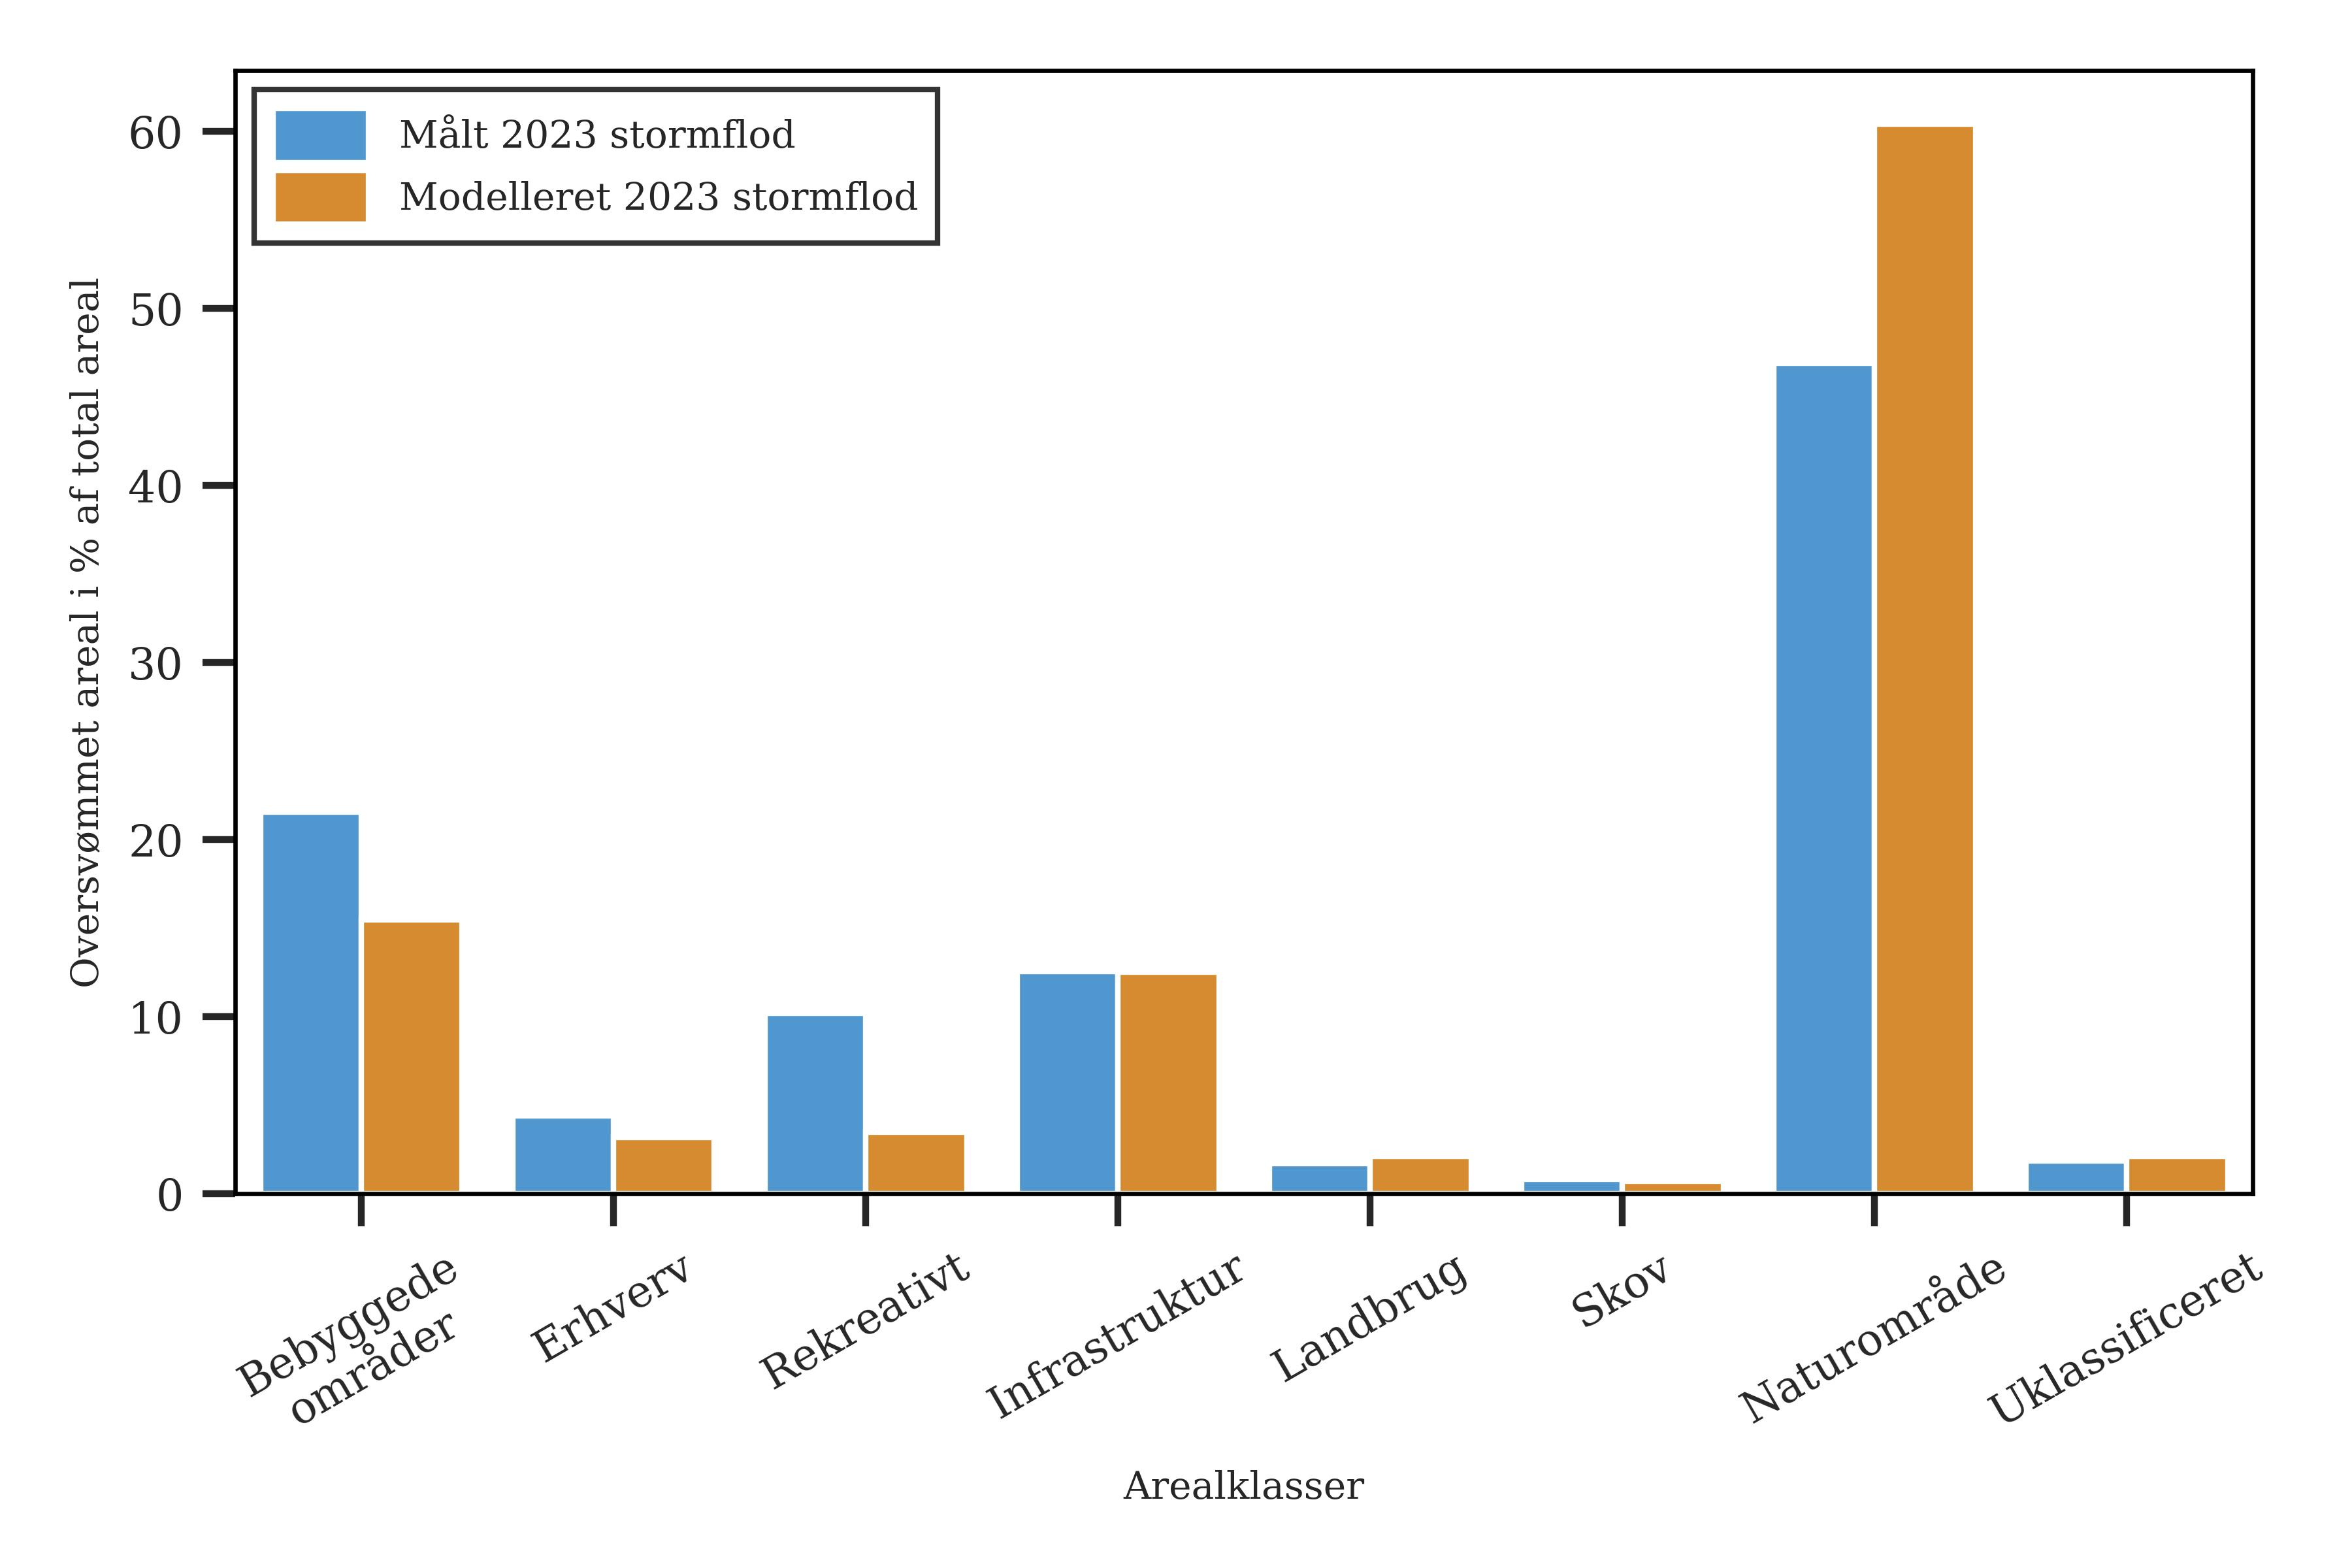
\includegraphics[width=1\linewidth]{images/Resultater/areal_anvendelses_grafer/praestoe_arealanvendelse.jpg}
        \caption{}
        \label{Subfig: Procent præstø}
    \end{subfigure}
    \begin{subfigure}[b]{0.5\textwidth}
        \centering
        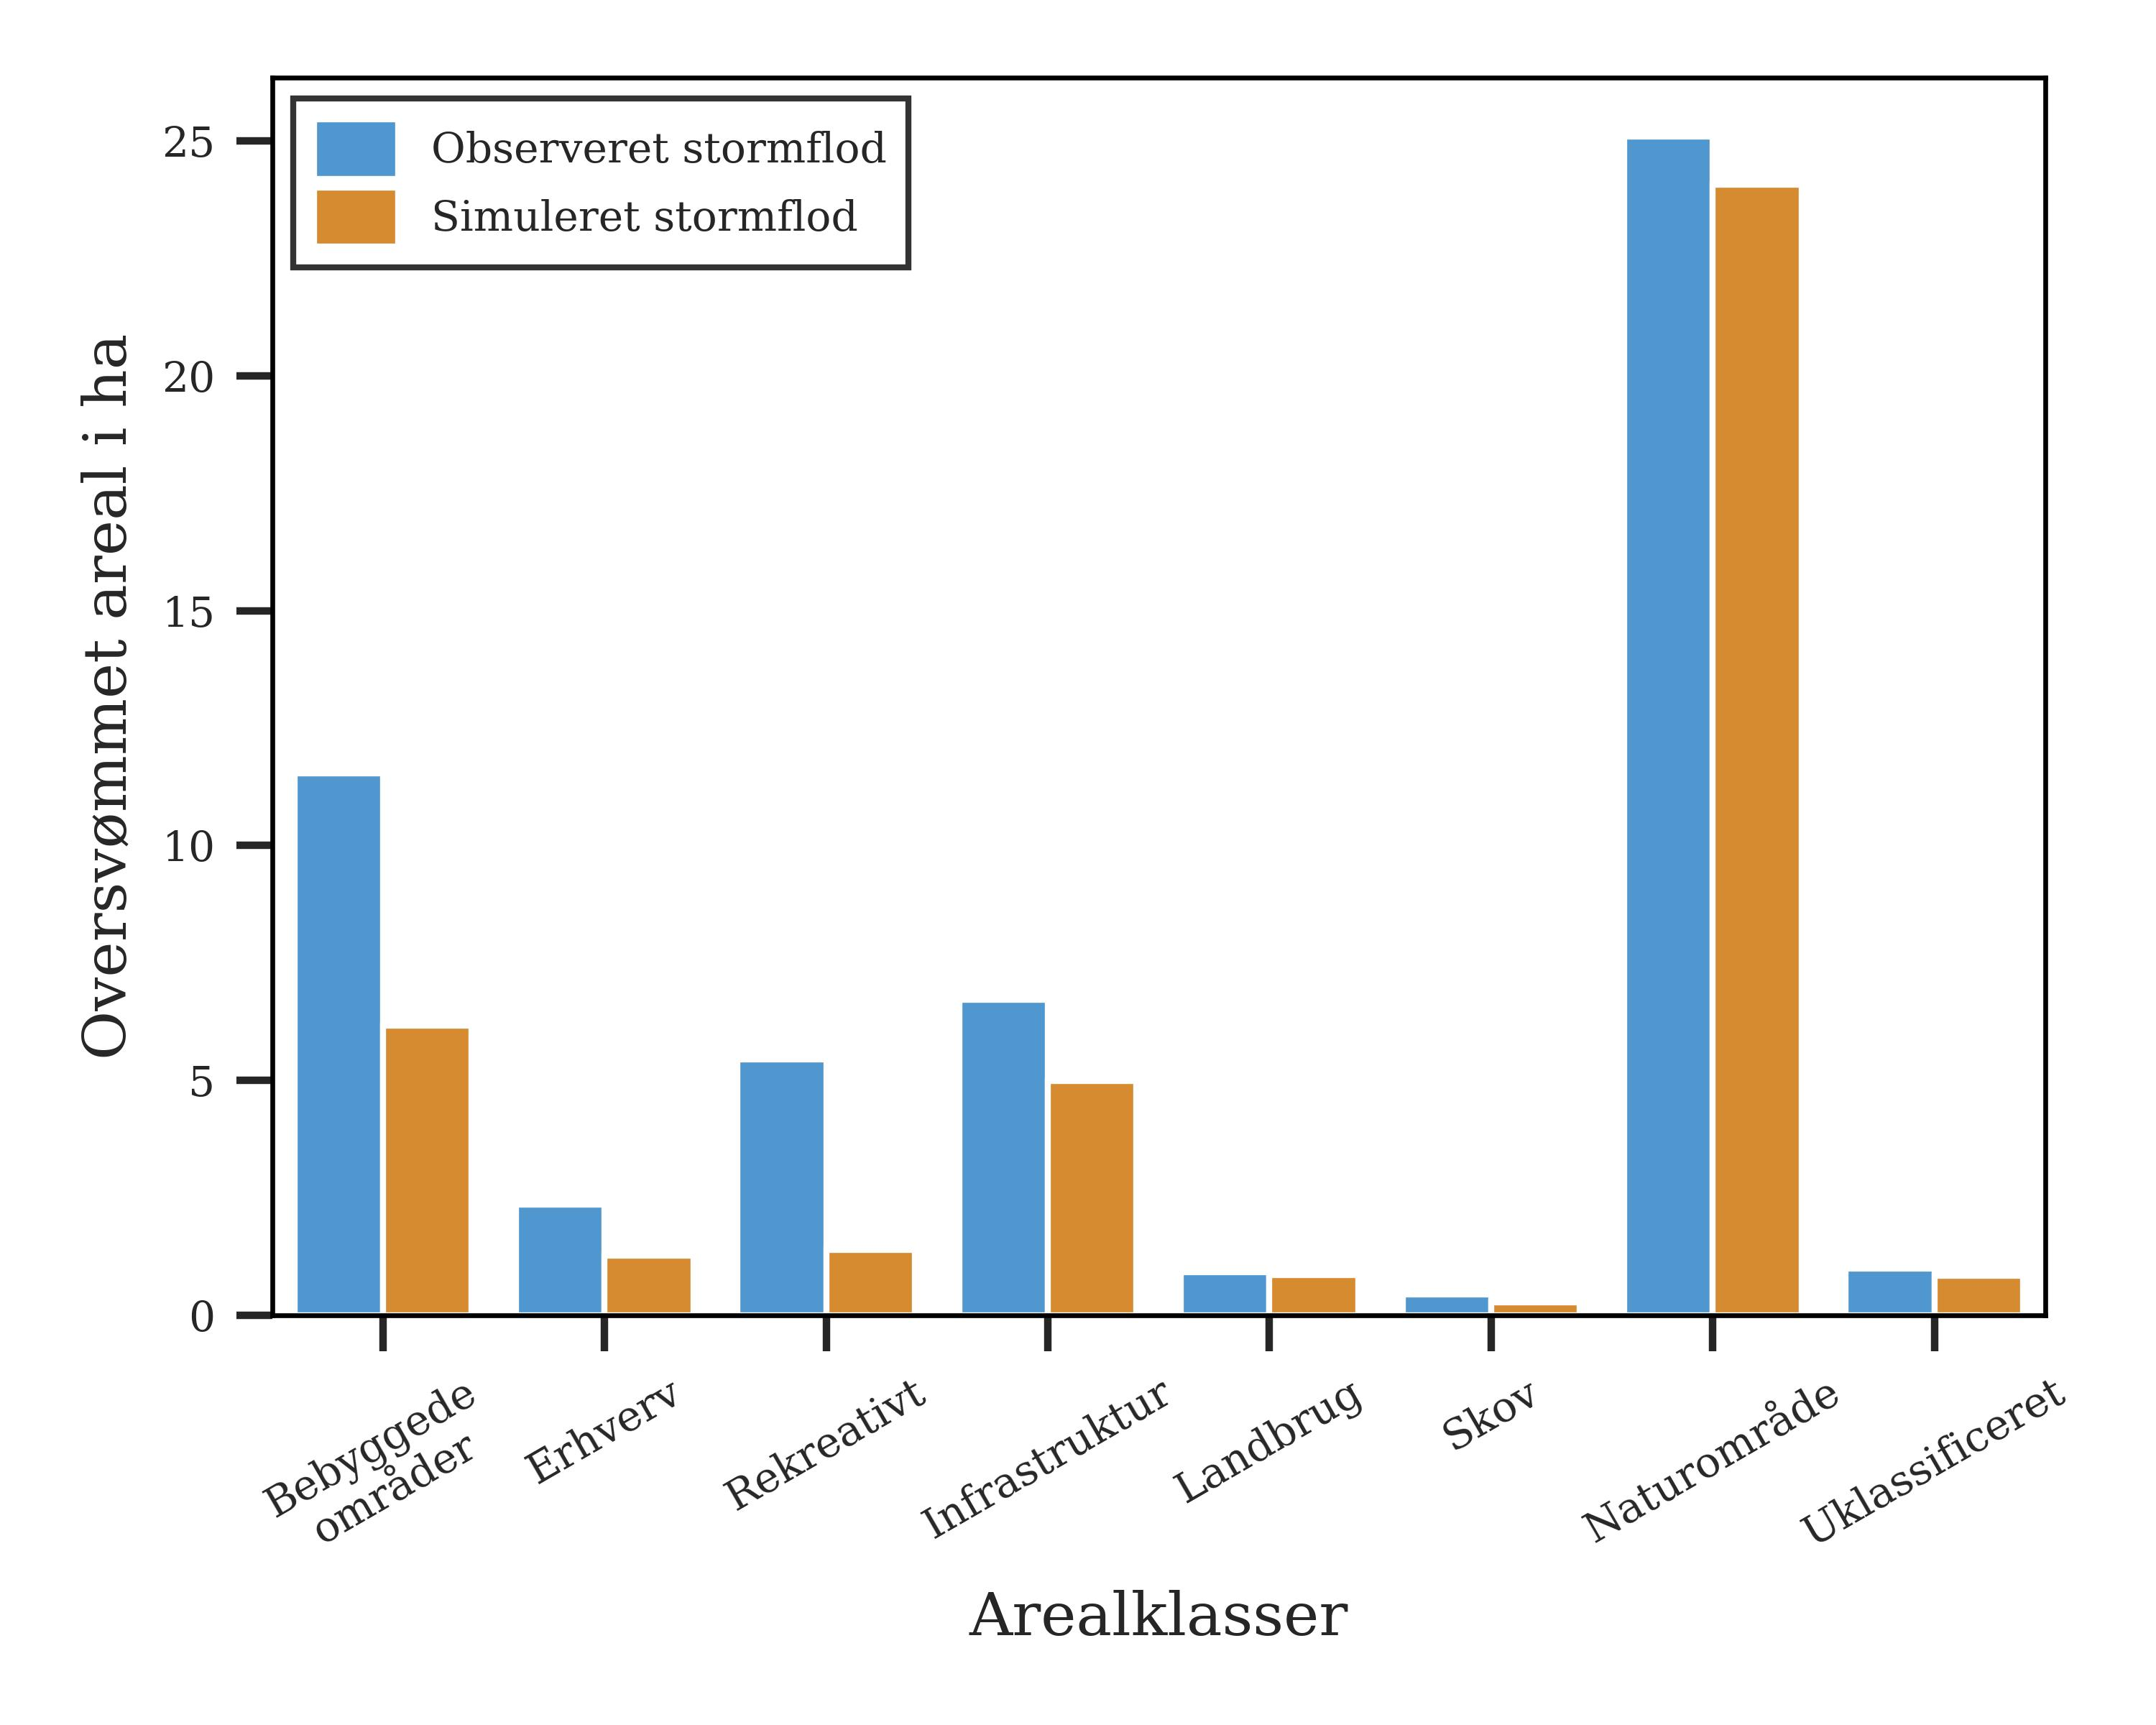
\includegraphics[width=1\linewidth]{images/Resultater/areal_anvendelses_grafer/praestoe_oversvommet_Hektar.jpg}
        \caption{}
        \label{Subfig: Hektar præstø}
    \end{subfigure}
    \caption{Påvirkede arealanvendelsesklasser i Præstø for den observeret og simuleret stormflod. \textbf{(a)} Oversømmet areal som procent af det totale areal. \textbf{(b)} Oversvømmet areal i hektar.}
    \label{Figur: Påvirket arealanvendelse Præstø}
\end{figure}



\subsection{Fremskrevet og statistiske stormflods hændelser}

I denne sektion vil der blive præsenteret resultaterne  af en statistisk 100-års hændelse og en fremskrivning af oktober 2023-stormfloden i slutningen af det nuværende århundrede ved et SSP4,5 og 8,5 udledningsscenarie. \\

I figur \ref{Figur: Klima Aabenraa} ses et oversvømmelseskort over Aabenraa for en statistisk 100-års hændelse og en fremskrivning af 2023 stormfloden ved et SSP4,5 og SSP8,5 scenarie. Det største areal oversvømmet sker ved en vandstand på 234 cm over DVR90. En større del af den sydlige bydel bliver oversvømmet ved en statistisk 100-års hændelse i et SSP4,5 scenarie. Oversvømmet areal ved fremskrivningen af stormfloden i et SSP8,5 scenarie er 13\% større end en statistisk 100-års hændelse i SSP4,5. Dette svarer til 19,6 ha. I forhold til den observeret stormflodshændelse, oversvømmer en fremskrevet stormflod et 96 og 104 ha større areal ved henholdsvis et SSP4,5 og SSP8,5 klimascenarie.
\begin{figure}[H]
    \centering
    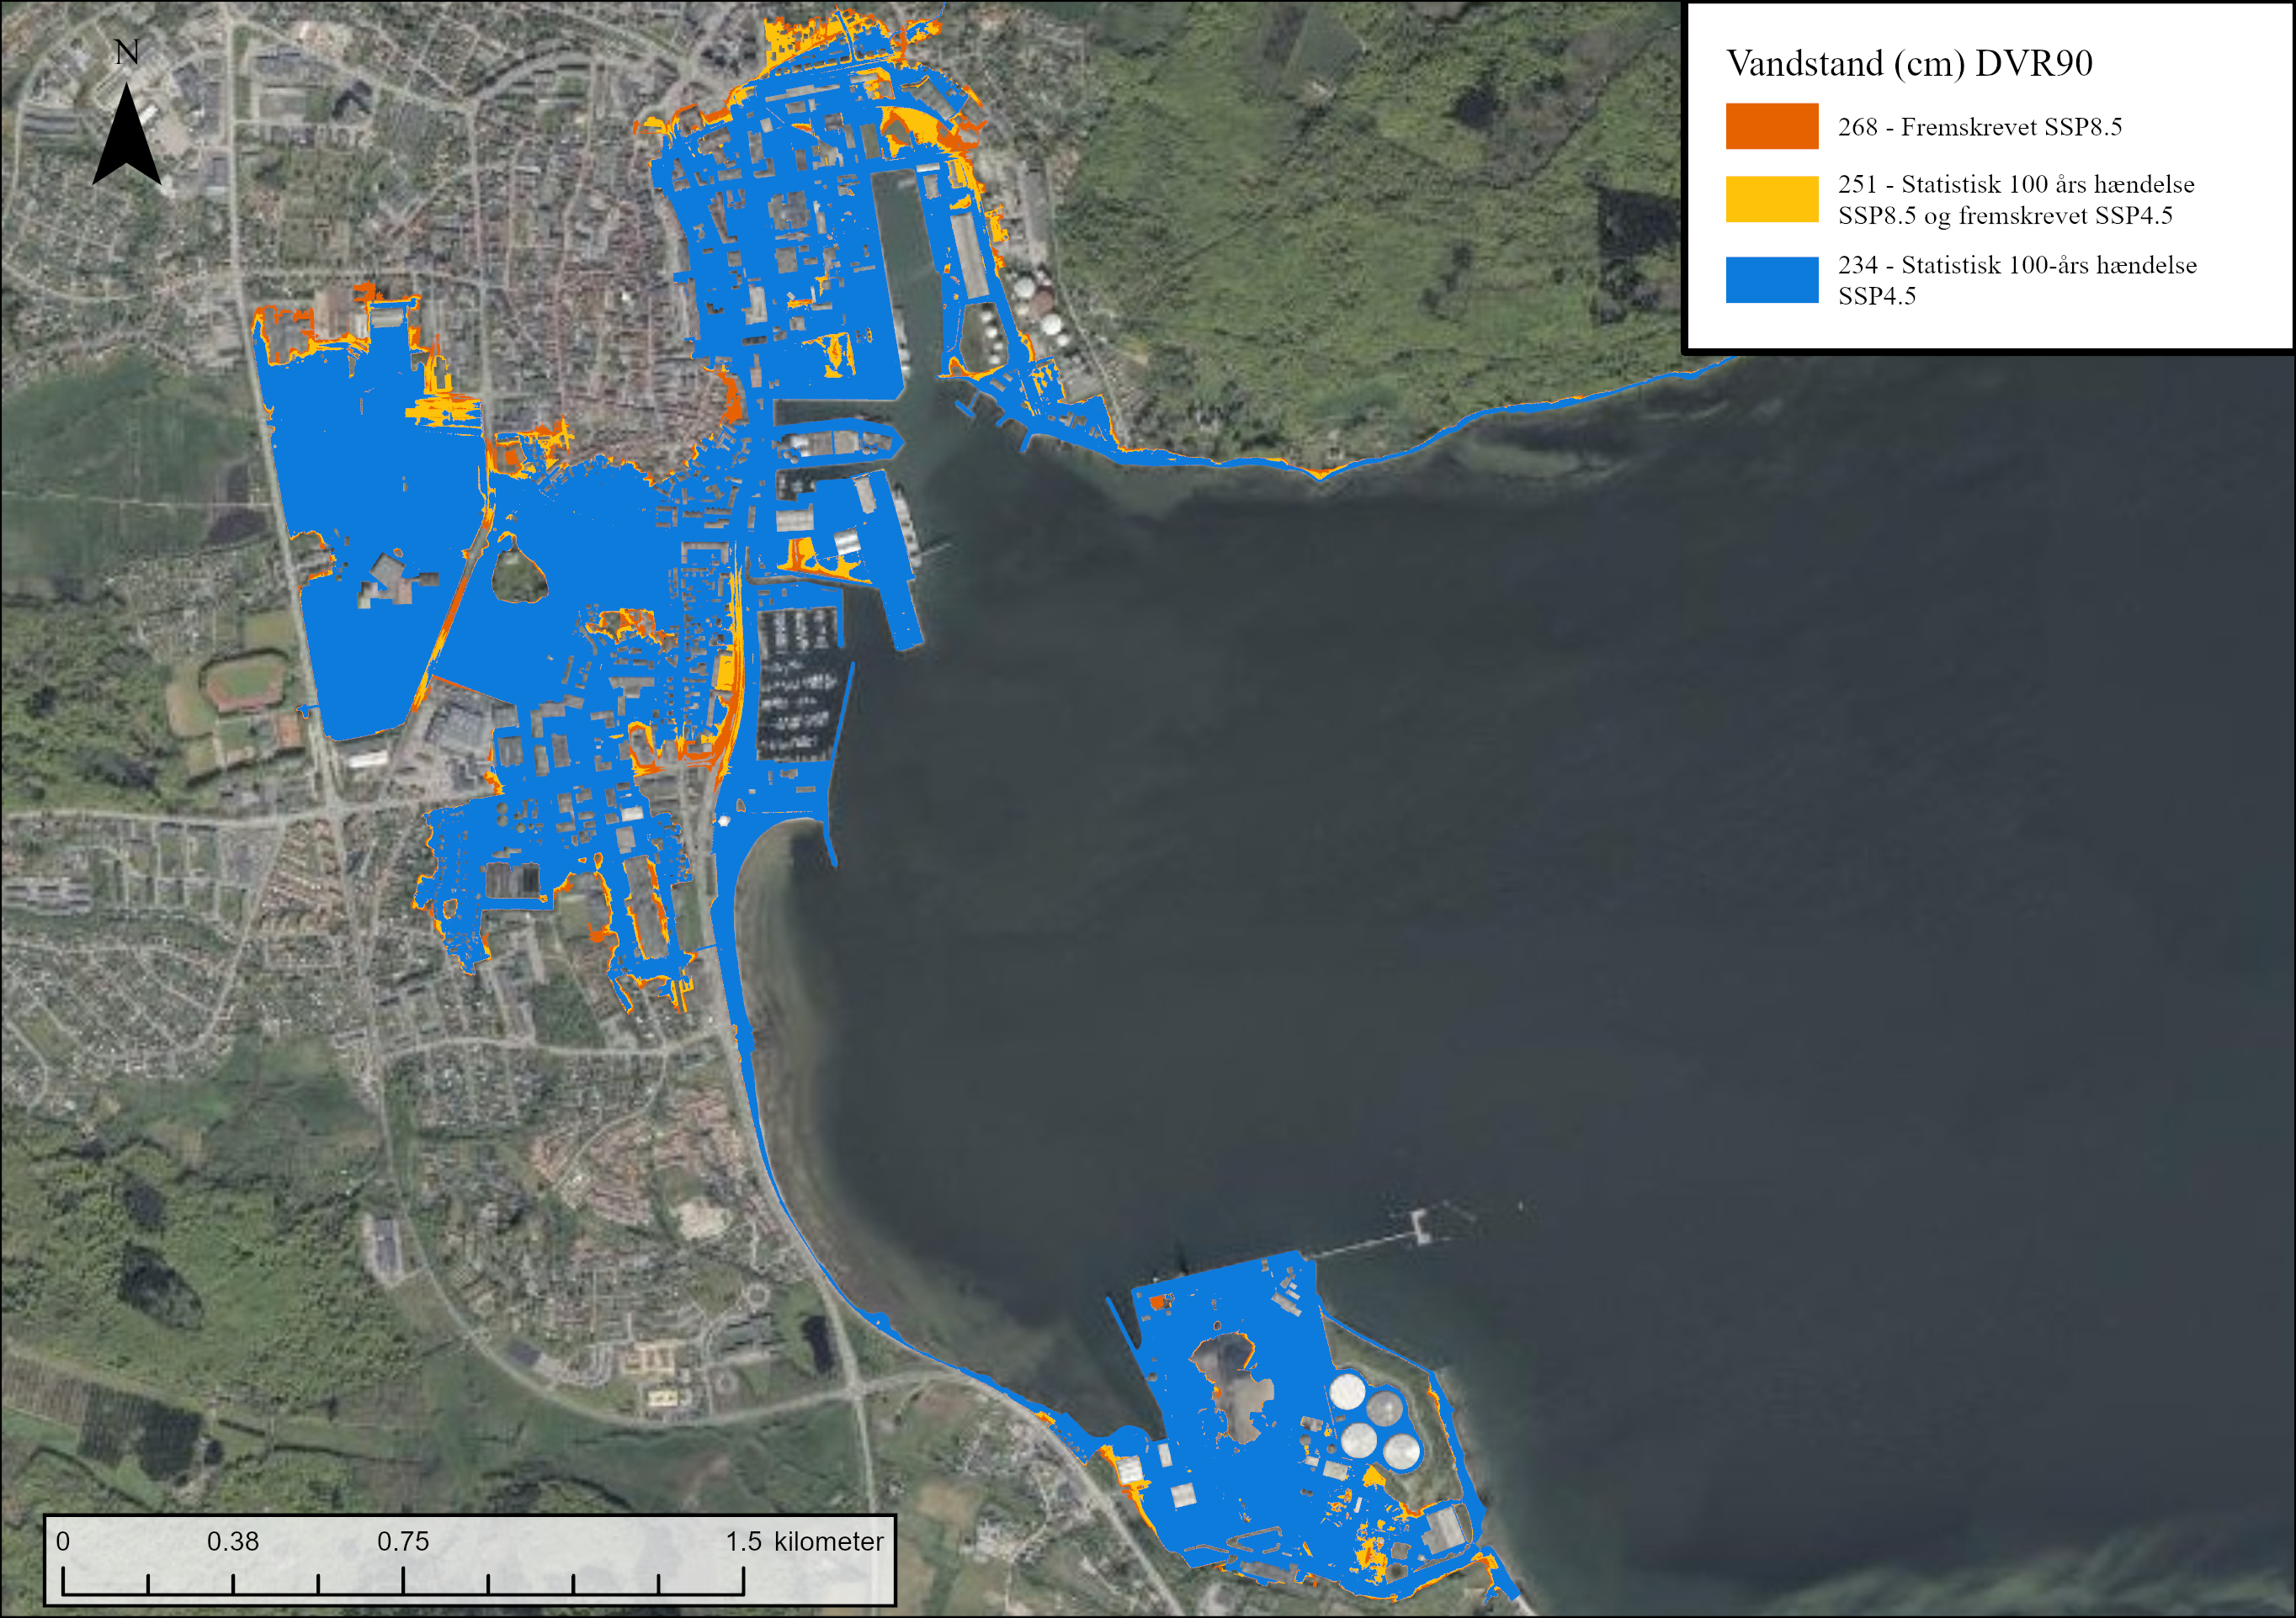
\includegraphics[width=0.8\linewidth]{images/Resultater/fremskrevet_hændelser/klima resultat_aabenraa.jpg}
    \caption{Kort over oversvømmet areal i Aabenraa af en stormflod ved en statistisk 100-års hændelse og en fremskrivning af oktober 2023 stormfloden til slutningen af århundredet ved SSP4,5 og SSP8,5 i centimeter over DVR90}
    \label{Figur: Klima Aabenraa}
\end{figure}

I figur \ref{Figur: Klima Gedser Havn} er der vist et oversvømmelseskort over Gedser Havn for en statistisk 100-års hændelse og fremskrivningen af oktober 2023 stormfloden ved et SSP4,5 og 8,5 scenarie. Den største del af oversvømmelsen sker ved en fremskrevet 2023 stormflod ved SSP4,5 med en vandstand på 220 cm DVR90. Størstedelen af landsbyen Gedser Havn bliver oversvømmet samt en del af det bagvedliggende landbrugsområder. Ved en statistisk 100-års hændelse i et SSP8,5 scenarie er det oversvømmet areal steget til 219,7 ha, en stigning på 537\% i forhold til den stormflod der ramte i oktober 2023. 

\begin{figure}[H]
    \centering
    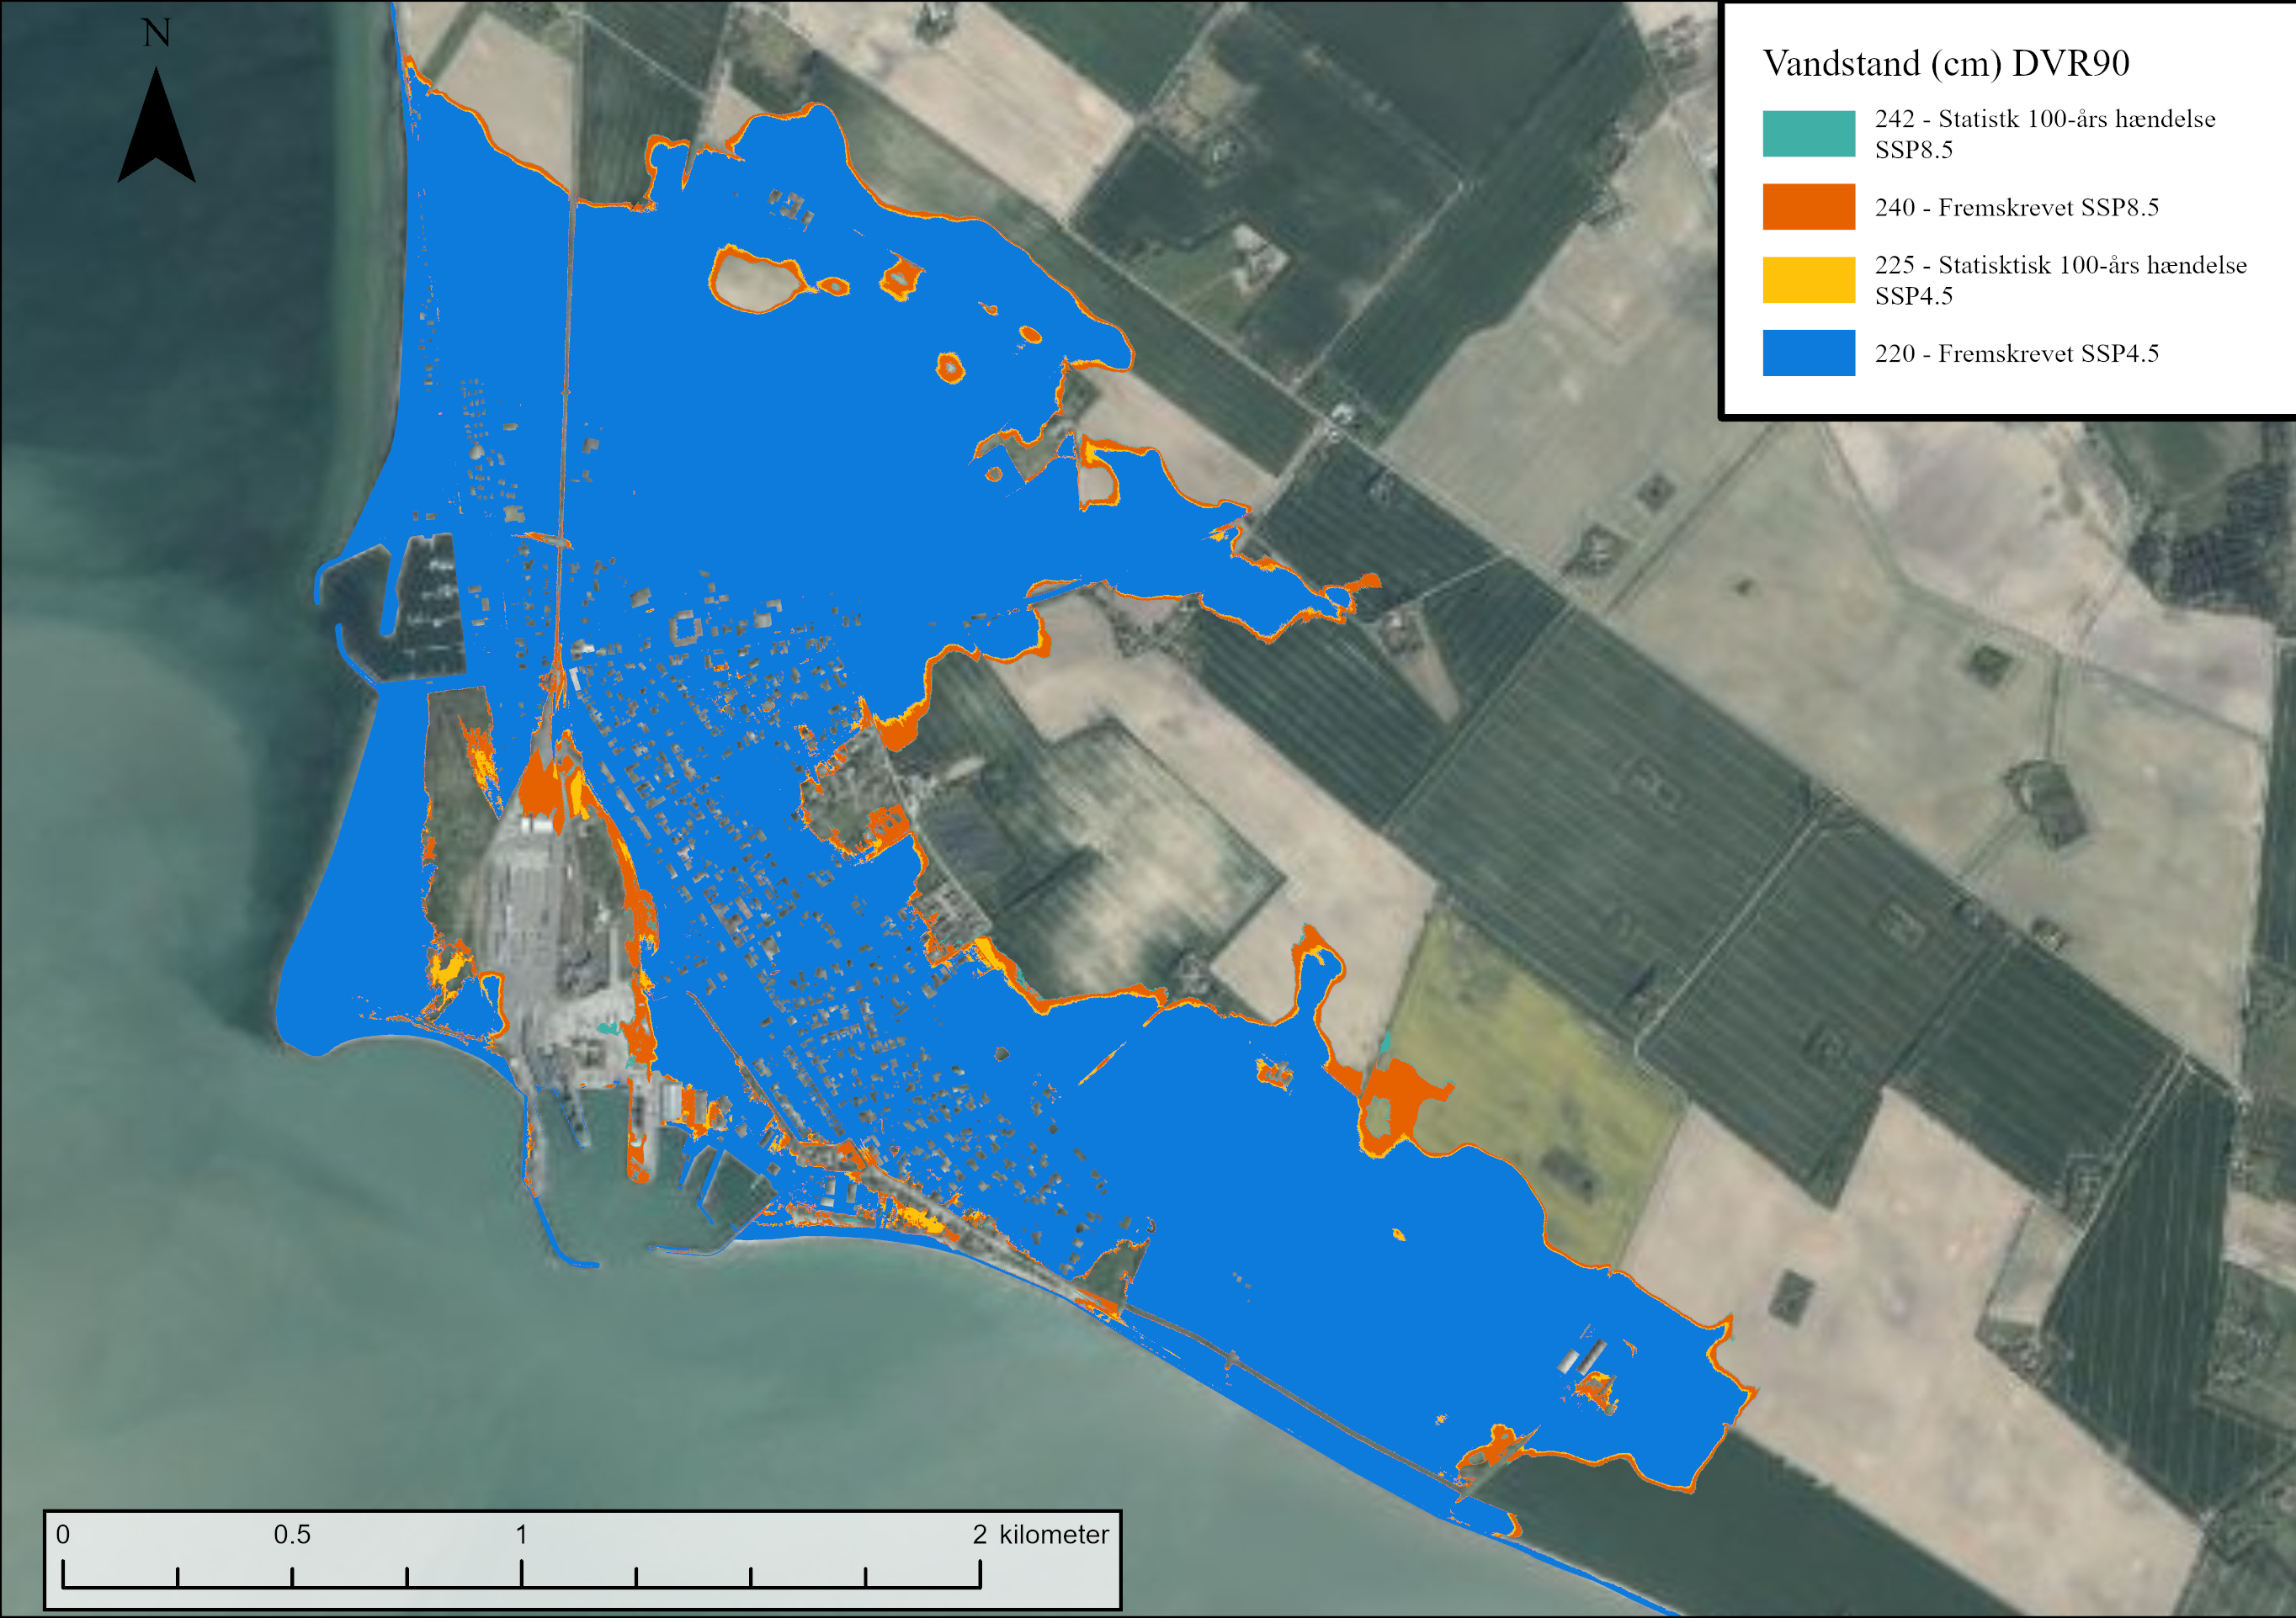
\includegraphics[width=0.8\linewidth]{images/Resultater/fremskrevet_hændelser/klima resultat gedser.jpg}
    \caption{Kort over oversvømmet areal i Gedser Havn af en stormflod ved en statistisk 100-års hændelse og en fremskrivning af oktober 2023 stormfloden til slutningen af århundredet ved SSP4,5 og SSP8,5 i centimeter over DVR90}
    \label{Figur: Klima Gedser Havn}
\end{figure}

I Hesnæs bliver et stort lavliggende græsareal oversvømmet ved en statistisk 100-års hændelse i et SSP8,5 scenarie. Ved en 100-års hændelse i SSP4,5 oversvømmes det meste af kysten og havnen. Selve Hesnæs by er udenfor oversvømmelsesrisiko selv ved det højeste vandstandsniveau på 259 cm DVR90 (figur \ref{Figur: Klima Hesnæs}). Ved en fremskrevet stormflod i et SSP8,5 scenarie vil det oversvømmede areal stige fra 4,8 ha til 114,8 ha. Dette er en stigning på 2273\%. \\
Ved en fremskrevet 2023 stormflod ved SSP8,5 vil der oversvømmes et areal der er 3219\% større end det der blev målt under stormfloden den 20. oktober 2023. Dette er en stigning på 111 ha. 

\begin{figure}[H]
    \centering
    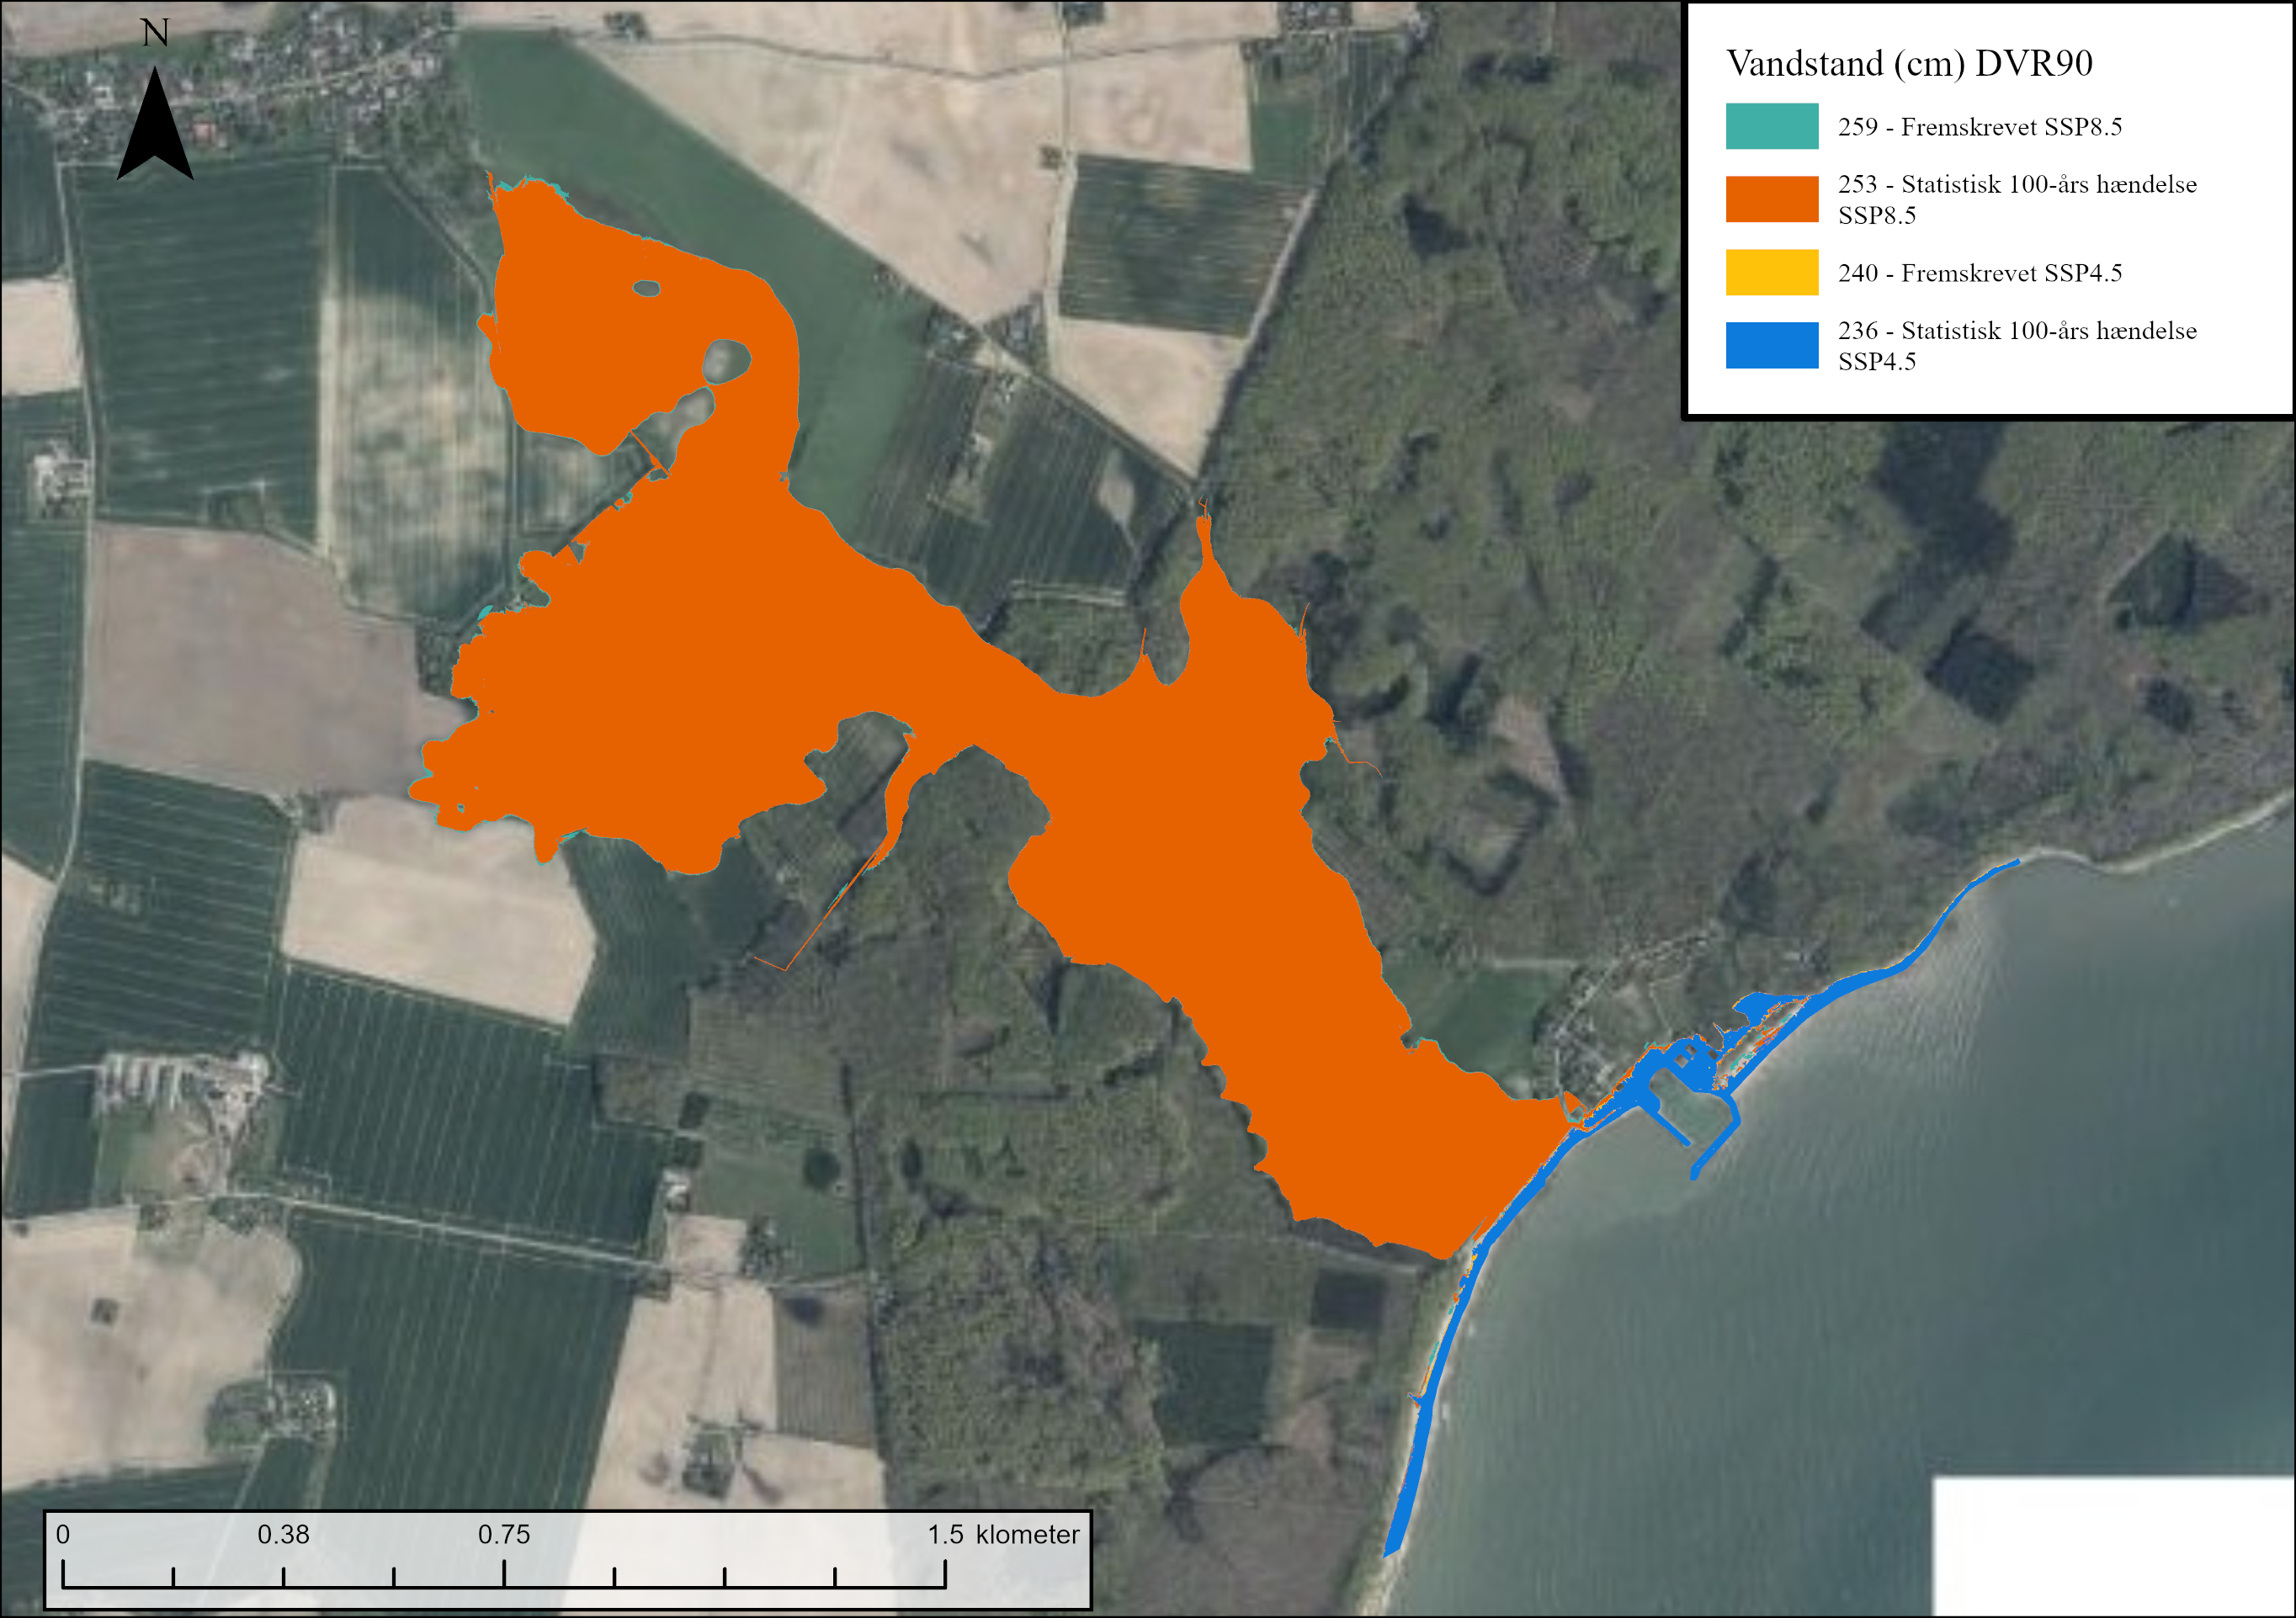
\includegraphics[width=0.8\linewidth]{images/Resultater/fremskrevet_hændelser/klima resultat hesnaes.jpg}
    \caption{Kort over oversvømmet areal i Hesnæs af en stormflod ved en statistisk 100-års hændelse og en fremskrivning af oktober 2023 stormfloden til slutningen af århundredet ved SSP4,5 og SSP8,5 i centimeter over DVR90}
    \label{Figur: Klima Hesnæs}
\end{figure}

I figur \ref{Figur: Klima Præstø} ses vandets udbredelse ved en statistisk 100-års hændelse og en fremskrevet stormflod i et SSP4,5 og 8,5 scenarie. Ved en 100-års SSP4,5 hændelse bliver dele af Præstø by oversvømmet, både nord og syd for Tubæk Ådal. Størstedelen af Tubæk Ådal vil også blive lagt under vand og åen vil gå over sine bredder i den sydlige del af byen. Et areal der er 68\% større end stormfloden der oversvømmede byen i 2023 vil blive oversvømmet hvis den samme stormflod rammer Præstø i slutningen af dette århundrede i et SSP8,5 scenarie. Dette svarer til et 36 ha større oversvømmet areal. 

\begin{figure}[H]
    \centering
    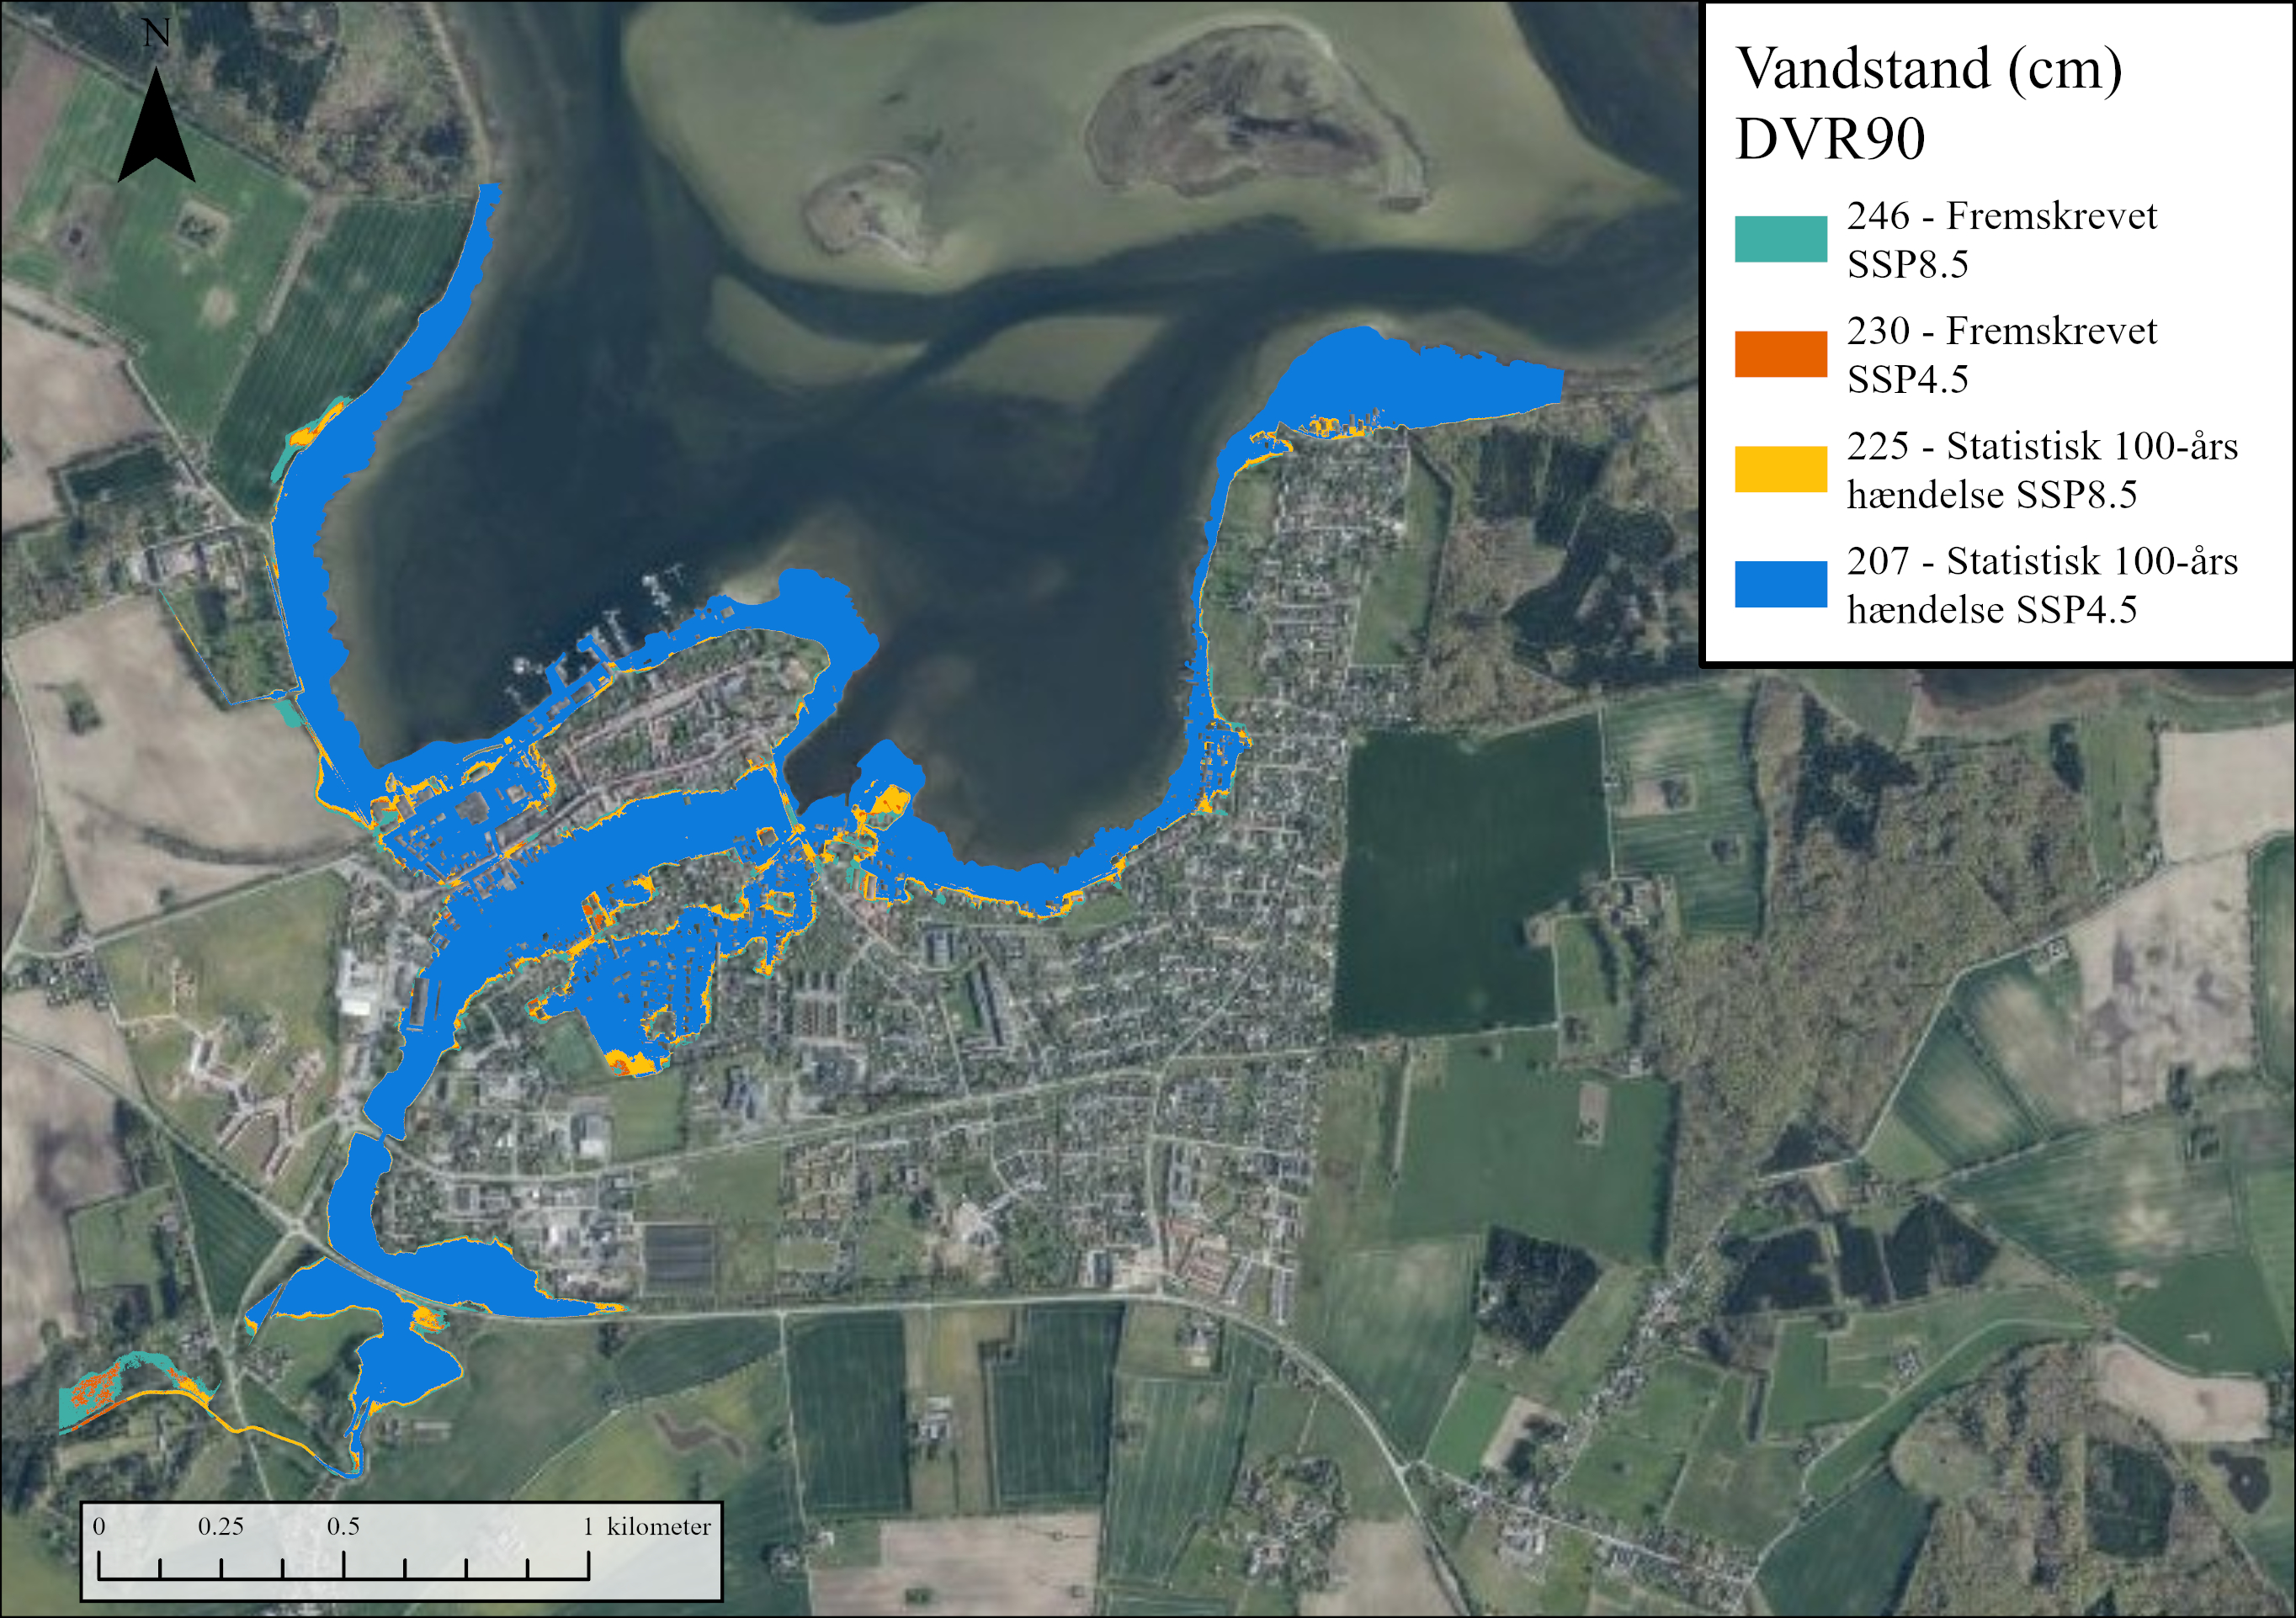
\includegraphics[width=0.8\linewidth]{images/Resultater/fremskrevet_hændelser/klima resultat praestoe.jpg}
    \caption{Kort over oversvømmet areal i Præstø af en stormflod ved en statistisk 100-års hændelse og en fremskrivning af oktober 2023 stormfloden til slutningen af århundredet ved SSP4,5 og SSP8,5 i centimeter over DVR90}
    \label{Figur: Klima Præstø}
\end{figure}

Sammenfattet bliver alle studieområderne påvirket af oversvømmelser ved stormfloder. I tabel \ref{Tabel: Oversvømmet arealer af stormfloder} er der blevet kvantificeret størrelsen af oversvømmelserne i hektar for alle hændelser modelleret af Inundation Modellen samt den observeret stormflod i 2023.\\ 
Det største oversvømmet areal er i Gedser Havn ved en fremskrevet 2023 stormflod i SSP8,5 på 219 ha og den mindste areal er simuleringen af 2023 stormfloden i Hesnæs på 3,3 ha. \\

\begin{table}[H]
\centering
\renewcommand{\arraystretch}{1.2} 
\begin{threeparttable}
\caption{Oversvømmet areal af den målte 2023-stormflod, den simuleret 2023-stormflod samt den statistiske 100-års hændelse og den fremskrevet 2023-stormflod til slutningen af århundredet ved SSP4.5 og 8.5 i hektar for hvert studieområde.}
\begin{tabular}{@{} l S[table-format=3.1, output-decimal-marker={,}] 
                    S[table-format=3.1, output-decimal-marker={,}] 
                    S[table-format=3.1, output-decimal-marker={,}] 
                    S[table-format=3.1, output-decimal-marker={,}] 
                    S[table-format=3.1, output-decimal-marker={,}] 
                    S[table-format=3.1, output-decimal-marker={,}] @{}} 
\toprule
& \multicolumn{1}{c}{\textbf{\makecell{Målt 2023\\stormflod}}} 
& \multicolumn{1}{c}{\textbf{\makecell{Simuleret 2023\\stormflod}}} 
& \multicolumn{2}{c}{\textbf{\makecell{Statistisk 100-års\\hændelse}}} 
& \multicolumn{2}{c}{\textbf{\makecell{Fremskrevet 2023\\stormflod}}} \\ 
\cmidrule(l){4-5} \cmidrule(l){6-7}
{\textit{ha}} & & & {\textit{SSP4.5}} & {\textit{SSP8.5}} & {\textit{SSP4.5}} & {\textit{SSP8.5}} \\
\midrule
  Aabenraa & 70,7 & 129,8 & 155,2 & 166,7 & 166,7 & 174,9 \\
  Gedser & 34,5 & 33,2 & 205,1 & 219,7 & 201 & 218,1 \\ 
  Hesnæs & 3.5 & 3,3 & 4,8 & 113,4 & 4,8 & 114,8 \\
  Præstø & 53,5 & 39,8 & 75,7 & 82 & 84,1 & 89,7 \\
\bottomrule
\end{tabular}
\label{Tabel: Oversvømmet arealer af stormfloder}
\end{threeparttable}
\end{table}


\begin{table}[H]
\centering
\begin{threeparttable}
\caption{Oversvømmet areal af den observeret 2023-stormflod, den simuleret 2023-stormflod samt den statistiske 100-års hændelse og den fremskrevet 2023-stormflod til slutningen af århundredet ved SSP4.5 og 8.5 i hektar og den procentvise forskel i forhold til 2023 stormfloden for hvert studieområde.}
\begin{tabular}{@{} l >{\centering\arraybackslash}m{0.13\textwidth} >{\centering\arraybackslash}m{0.13\textwidth} >{\centering\arraybackslash}m{0.13\textwidth} >{\centering\arraybackslash}m{0.13\textwidth} >{\centering\arraybackslash}m{0.13\textwidth} >{\centering\arraybackslash}m{0.13\textwidth} @{}} 
\toprule
& \textbf{\makecell{Målt 2023\\stormflod}} 
& \textbf{\makecell{Simuleret 2023\\stormflod}} 
& \multicolumn{2}{c}{\textbf{\makecell{Statistisk 100-års\\hændelse}}} 
& \multicolumn{2}{c}{\textbf{\makecell{Fremskrevet 2023\\stormflod}}} \\ 
\cmidrule(l){4-5} \cmidrule(l){6-7}
{\textit{ha}} & & & {\textit{SSP4.5}} & {\textit{SSP8.5}} & {\textit{SSP4.5}} & {\textit{SSP8.5}} \\
\midrule
\renewcommand{\arraystretch}{1.2}
Aabenraa & 70,7 & 129,8 (+84\%) & 155,2 (+119\%) & 166,7 (+136\%) & 166,7 (+136\%) & 174,9 (+147\%)\\
Gedser   & 34,5 & 33,2 (-4\%) & 205,1 (+495\%)& 219,7 (+537\%)& 201,0 (+483\%)& 218,1 (+533\%)\\ 
Hesnæs   & 3,5  & 3,3 (-5\%) & 4,8 (+38\%)  & 113,4 (+3181\%) & 4,8 (+40\%) & 114,8 (+3220\%)\\
Præstø   & 53,5 & 39,8 (-26\%)& 75,7 (+42\%)& 82,0 (+53\%)& 84,1 (+57\%)& 89,7 (+68\%)\\
\bottomrule
\end{tabular}
\label{Tabel: Oversvømmet arealer af stormfloder i hektar}
\end{threeparttable}
\end{table}
 